\chapter{Cryogenic Instrumentation and Slow Control}
\label{ch:sp-cisc}

%%%%%%%%
\section{Overview} \fixme{I strongly suggest dropping this as a heading. You may want to rethink the headings a bit. The first section is an overview, so go right to the Introduction as a heading, and Components, Scope, and Requirements as subheadings under Introduction.}

\subsection{Introduction}

% \fixme{SG: Done. Editors, please check --- Looks good [gahs]}


The \dword{cisc} system provides comprehensive monitoring for all \dword{detmodule} components as well as \lar quality and behavior, both crucial to guarantee high-quality data. Beyond passive monitoring, \dword{cisc} also provides a control system for some of the detector components. The structure of the \dword{cisc} consortium is quite
complex. Figure~\ref{fig:cisc-subsystem-chart} provides a subsystem chart for the \dword{cisc} system. 

\begin{dunefigure}[\dword{cisc} subsystem chart]{fig:cisc-subsystem-chart}
  {\dword{cisc} subsystem chart}
  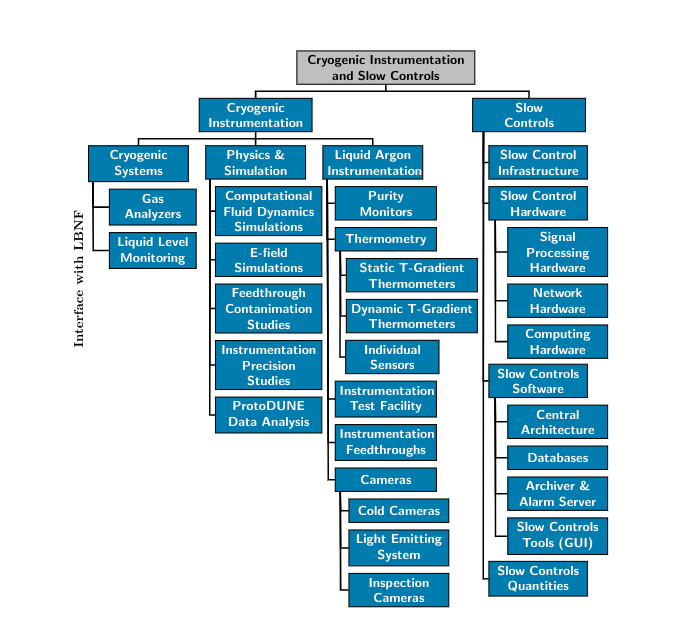
\includegraphics[width=0.6\textwidth]{CISC_scope-v3_TDR.png}
\end{dunefigure}

\dword{cisc} has two main branches: cryogenics instrumentation and slow controls. The former includes a set of instrumentation devices to monitor the quality and behavior of the \lar volume in the cryostat interior, ensuring correct functioning of the full cryogenics system and suitability of the \lar for good quality physics data. The second branch of \dword{cisc} is the slow controls (SC) system, in charge of monitoring and controlling most detector elements: power supplies, electronics, racks, instrumentation devices, calibration devices, among others. \fixme{This should be a complete list.}

For all \lar instrumentation devices, \dword{pdsp} designs are
the baseline, and requirements for most design
parameters are extrapolated from \dword{pdsp}. Hence, the \dword{pdsp} data will be used to validate the instrumentation designs and to understand their performance.

\subsection{Components}
% \fixme{SG: Done. Editors, please check --- looks good [gahs]}

The devices included under cryogenics instrumentation are purity monitors,  different types of temperature monitors, and cameras with their associated light emitting systems. Also included are components like gas analyzers and \lar level monitors that are directly related to the external cryogenics system and thus have substantial interfaces with \dword{lbnf}. A test facility for the instrumentation devices is also included as part of the cryogenics instrumentation.

Cryogenics instrumentation also requires significant physics and
simulation work such as \efield simulations and cryogenics modeling
studies using \dfirst{cfd}. \efield simulations
are required to identify desirable locations for instrumentation
devices in the cryostat, so they are not in regions of high \efield, and their presence does not induce large field distortions. 
% AC. What do we mean by distortions here ?
% Alternative: ``that their designs do not induce high \efields and risk of dielectric breakdown. ``
\dshort{cfd} simulations are needed to understand expected temperature, impurity, and velocity flow distributions and guide the placement and distribution of instrumentation devices inside the cryostat.

The slow controls has three main components: hardware, infrastructure, and software. The slow controls hardware and infrastructure comprises networking hardware, signal processing hardware, computing hardware, and relevant rack infrastructure. The slow controls software is needed for signal processing, alarms, archiving, and control room displays.

\subsection{Scope}
%\fixme{SG: Done. Editors, please check --- GAHS: added a few words, please check; SG: Checked, looks good!}

As described in the previous section, and shown schematically in Figure~\ref{fig:cisc-subsystem-chart}, the scope of the \dword{cisc} system spans a broad range of activities. For the cryogenics systems (gas analyzers and liquid level monitors), \dword{lbnf} provides the needed expertise and is responsible for the design, installation, and commissioning while the \dword{cisc} consortium provides the resources and supplements labor as needed. For \dword{lar} instrumentation devices (purity monitors, thermometers, cameras, and light-emitting system, and their associated feedthroughs) and instrumentation test facility, CISC is responsible for design through commissioning in the \dwords{fd}.

For slow controls, \dword{cisc} provides software and infrastructure for controlling and monitoring all detector elements that provide data on the health of the detector module or conditions important to the experiment, as well some related hardware. Slow controls includes the systems detailed below:

\textbf{Slow controls base software and databases:} provides the central tools needed to develop
control and monitoring for various detector systems and interfaces.
\begin{itemize}
\item Base input/output software,
\item Alarms; archiving; display panels; operator interface tools,
\item Slow controls system documentation and operations guidelines.
\end{itemize}
%
\textbf{Slow controls for external systems:} export data from systems external to the detector and provide status monitoring for operators and archiving.
\begin{itemize}
\item Beam status; cryogenics status; data acquisition (DAQ) status; facilities systems status,
\item For the systems above, import other interesting monitoring data as needed (e.g., pumps
data from cryogenics system, heaters data from facility systems), \fixme{Beginning the list with "e.g." eliminates the need for "etc." at the end. Etc. is not a good term to use in lists anyway.}
\item Building controls; detector hall monitoring; ground impedance monitoring,
\item Interlock status bit monitoring (but not the actual interlock mechanism).
\end{itemize}
%
\textbf{Slow controls for detector hardware systems:} develop software interfaces for detector hardware devices.
\begin{itemize}
\item Monitoring and control of all power supplies,
\item Full rack monitoring (rack fans, thermometers and rack protection system),
\item Instrumentation and calibration device monitoring (and control to the extent needed),
\item Power distribution units monitoring; computer hardware monitoring,
\item High voltage system monitoring through cold cameras,
\item Detector components inspection through warm cameras.
\end{itemize}
%
\textbf{Slow controls hardware:} \dword{cisc} will develop, install, and commission any hardware related to rack monitoring and control. Most power supplies may only need a cable from the device
to an Ethernet switch, but some power supplies might need special cables ({\em e.g.} \fixme{Previous examples of e.g. were not in italics. This should be consistent throughout the document. This may be something that requires an overall find and replace once the entire document is finished.} , GPIB or RS232) for communication. The \dword{cisc} consortium will be responsible for providing these control cables.

In addition to the listed activities, \dword{cisc} also has activities outside the scope of the consortium that require coordination with other groups. This is discussed in Sec.~\ref{sec:interfaces}.

\subsection{Requirements}
%\fixme{GAHS: text looks good; some numbers need to be replaced with latex commands from defs.tex or parameters.tex}

Some common design considerations for instrumentation devices include stability, reliability, and longevity so that the devices can survive for a period of at least \dunelifetime. \fixme{The preview shows "20 year." That should be plural (years).} For any device to have such a long lifetime is uncommon, so the overall design allows replacing devices where possible. As for any other element inside the cryostat, the \efield  on the instrumentation devices must be less than \localefield to minimize the risk of dielectric breakdown in \dword{lar}. Another important design parameter, which should be evaluated in \dword{pdsp}, is the maximum noise level induced by instrumentation devices on the readout electronics that can be tolerated to avoid confusing event reconstruction. \fixme{I suggest the following rephrase: To avoid confusing event reconstruction, we include another important design parameter that should be evaluated in \dword{pdsp}: the maximum noise level induced by instrumentation devices on the readout electronics that can be tolerated.} Tables~\ref{tab:fdgen-slow-cryo-requirements-1} and \ref{tab:fdgen-slow-cryo-requirements-2} show the full set of requirements for the \dword{cisc} subsystems.
% \todo{SG: In table 1.2, there are "(???)" next to heat transfer. Needs to be fixed.  GAHS: fixed.}

Data from purity monitors and different types of thermometers will be used to validate the liquid argon fluid flow model. A number of requirements drive the design parameters for these systems to achieve the needed precision and granularity in their distribution across the cryostat. For example, the electron lifetime measurement precision must be 1.4\% to keep the bias on the charge readout in the \dword{tpc} below 0.5\% at 3~ms lifetime. For thermometers, the requirements are driven by the \dshort{cfd} simulations based on \dword{pdsp} design. The resolution and relative precision of temperature measurements
\footnote{The resolution is defined as the temperature RMS for individual measurements and is driven by the electronics. The relative precision also includes the effect of reproducibility for successive inversions in LAr.}
must be less than 2~mK and 5~mK, respectively. \fixme{So the resolution is less than 2~mK, and the relative precision is less than 5~mK? I strongly suggest, under the circumstances to rephrase, if that is the case, to eliminate "respectively." Try this: The resolution of temperature measurements should be less than 2~mK, and the relative precision of those measurements should be less than 5~mK.} The relative precision is particularly important because gradients below 20~mK should be characterized.  
As will be described below, the laboratory calibration data and the recent analysis of thermometer instrumentation data from \dword{pdsp} does show that a 2.5~mK relative precision is achievable. 

The level meters must have a precision of 0.1\% over 14~m (14~mm) for measurement accuracy during filling. This precision is also sufficient for \dword{sp} to ensure the \dword{lar} level is above the ground planes. As shown in Table~\ref{tab:fdgen-slow-cryo-requirements-2}, several requirements drive the design of cold and warm cameras and the associated light emitting system. The components of the camera systems must not contaminate the liquid argon or produce bubbles when the \dword{hv} is on because that increases the risk of \dword{hv} discharge. Both cold and warm cameras must provide coverage of at least 80\% of the \dword{tpc} with a resolution of 1~cm for cold cameras and 2~mm for warm cameras on the \dword{tpc}.
% CEL: my 'fixme' with details, removed. Wanted to hold 
% if needed later in the document. 

For the cryogenic test facility, a cryostat with a capacity of 0.5 to approximately 3 cubic meter is reasonable because turn-around times and filling costs are lower for smaller cryostats. For gas analyzers, the operating range is an important requirement; details  are in Table~\ref{tab:fdgen-slow-cryo-requirements-1}.

For slow controls, the system must be designed to be sufficiently robust to support a large number of monitored variables, at a minimum of 50,000 variables, and a broad range of monitoring and archiving rates. The system must also be capable of an interface with a large number of detector sub-systems to establish two-way communication for control and monitoring. 

% \fixme{Requirements table: replace ALARA with number or clear criterion, per reviewer comments. [gahs]; SG: I suggest using ENC < 1000 e$^{-}$ for minimum requirement and ALARA as goal. --- done [gahs]}
\fixme{Anne adds input of generated SP-CISC specifications table here. Need to compare contents and make sure the generated one contains all the right information for the CISC-specific items. The top-level ones that apply are separate and will be coming soon. (12/17)}
% This file is generated, any edits may be lost.

\begin{longtable}{p{0.14\textwidth}p{0.13\textwidth}p{0.18\textwidth}p{0.22\textwidth}p{0.20\textwidth}}
\caption{Specifications for SP-CISC \fixmehl{ref \texttt{tab:spec:SP-CISC}}} \\
  \rowcolor{dunesky}
       Label & Description  & Specification \newline (Goal) & Rationale & Validation \\  \colhline

    \\ \rowcolor{dunesky} \newtag{SP-FD-1}{ spec:min-drift-field } & Name: Minimum drift field \\
    Description & The drift field in the TPC shall be greater than 250 V/cm, with a goal of 500 V/cm.   \\  \colhline
    Specification (Goal) &  $>$\,\SI{250}{ V/cm}  ( $>\,\SI{500}{ V/cm}$ ) \\   \colhline
    Rationale &   Lessens impacts of e-Ar recombination, e-lifetime, e-diffusion and space charge.  \\ \colhline
    Validation & ProtoDUNE  \\
   \colhline

   
  \newtag{SP-FD-2}{ spec:system-noise }  & System noise  &  $<\,\SI{1000}\,e^-$ &  Provides $>$5:1 S/N on induction planes for  pattern recognition and two-track separation. &  ProtoDUNE and simulation \\ \colhline
    
    \\ \rowcolor{dunesky} \newtag{SP-FD-3}{ spec:light-yield } & Name: Light yield \\
    Description & The light yield shall be sufficient for measuring event time (and total intensity) of events with visible energy above 200 MeV.  Goal is to make possible a 10\% energy measurement for events with a visible energy of 10 MeV.   \\  \colhline
    Specification (Goal) &  $>\,\SI{0.5}{pe/MeV}$  ( $>\,\SI{5}{pe/MeV}$ ) \\   \colhline
    Rationale &   Rejects nucleon decay backgrounds from cosmogenic events near cathode.  \\ \colhline
    Validation &   \\
   \colhline

   \newtag{SP-FD-4}{ spec:time-resolution-pds }  & Time resolution  &  $<\,\SI{1}{\micro\second}$ \newline ( $<\,\SI{100}{\nano\second}$ ) &  Enables \SI{1}{mm} position resolution for \SI{10}{MeV} SNB candidate events for instantaneous rate $<\,\SI{1}{m^{-3}ms^{-1}}$. &   \\ \colhline
    
    \\ \rowcolor{dunesky} \newtag{SP-FD-5}{ spec:lar-purity } & Name: Liquid argon purity \\
    Description & The LAr purity shall remain lower than 100 ppt (with a goal of < 30 ppt). This corresponds to e- lifetime of 3 (10) ms.   \\  \colhline
    Specification (Goal) &  $<$\,\SI{100}{ppt}  ( $<\,\SI{30}{ppt}$ ) \\   \colhline
    Rationale &   Provides $>$5:1 S/N on induction planes for  pattern recognition and two-track separation.  \\ \colhline
    Validation & Purity monitors and cosmic ray tracks  \\
   \colhline

    \\ \rowcolor{dunesky} \newtag{SP-FD-15}{ spec:lar-n-contamination } & Name: LAr nitrogen contamination \\
    Description & The nitrogen contamination in the LAr shall remain below 25 ppm in order not to significantly affect the number of photons that reach the detectors (for both fast and late light components).   \\  \colhline
    Specification &  $<\,\SI{25}{ppm}$ \\   \colhline
    Rationale &   Maintain \SI{0.5}{PE/MeV} PDS sensitivity required for triggering proton decay near cathode.  \\ \colhline
    Validation & In situ measurment  \\
   \colhline

    \\ \rowcolor{dunesky} \newtag{SP-FD-18}{ spec:cryo-monitor-devices } & Name: Cryogenic monitoring devices \\
    Description & CISC shall provide sufficient instrumentation  to validate the fluid flow model, which constrains the level of purity inhomogeneities within the liquid.    \\  \colhline
    Specification &   \\   \colhline
    Rationale &   Constrain uncertainties on detection efficiency, fiducial volume.  \\ \colhline
    Validation & ProtoDUNE  \\
   \colhline

   
  \newtag{SP-FD-25}{ spec:non-fe-noise }  & Non-FE noise contributions  &  $<<\,\SI{1000}\,e^- $ &  High S/N for high reconstruction efficiency. &  Engineering calculation and ProtoDUNE \\ \colhline
    

    \\ \rowcolor{dunesky} \newtag{SP-CISC-1}{ spec:inst-noise } & Name: Noise from Instrumentation devices \\
    Description & The instrumentation devices shall contribute no more than \SI{1000}{enc} of noise, with a goal of ALARA. This requirement is on total system noise;   \\  \colhline
    Specification (Goal) &  $\ll\,\SI{1000}{enc}$  ( ALARA ) \\   \colhline
    Rationale &   Top level spec 25  \\ \colhline
    Validation &   \\
   \colhline

    \\ \rowcolor{dunesky} \newtag{SP-CISC-2}{ spec:inst-efield } & Name: Max. E field near instrumentation devices \\
    Description & The maximum field near instrumentation devices should be $<\,\SI{30}{kV/cm}$ to avoid dielectric breakdowns.   \\  \colhline
    Specification (Goal) &  $<\,\SI{30}{kV/cm}$  ( $<\,\SI{15}{kV/cm}$ ) \\   \colhline
    Rationale &   Significantly lower than max field of 30 kV/cm per DUNE HV   \\ \colhline
    Validation & 3D electrostatic simulation  \\
   \colhline

    \\ \rowcolor{dunesky} \newtag{SP-CISC-3}{ spec:elec-lifetime-prec } & Name: Precision in electron lifetime \\
    Description & The precision on the measurement of the electron lifetime needs to sufficient to ensure $<$ 0.5\% uncertainty in charge readout.   \\  \colhline
    Specification (Goal) &  $<\,$1.4\% ($<$4\%)  ( $<\,$1\% ) \\   \colhline
    Rationale &     \\ \colhline
    Validation &   \\
   \colhline

    \\ \rowcolor{dunesky} \newtag{SP-CISC-4}{ spec:elec-lifetime-range } & Name: Range in electron lifetime \\
    Description & The purity monitors inside the cryostat should be capable of measuring a lifetime range between 0 and 10 ms. The goal for the inline purity monitors is to measure a range of 0 to 30 ms for the drift electron lifetime.   \\  \colhline
    Specification (Goal) &  \SIrange{0}{10}{ms} (\SIrange{0}{30}{ms})  ( \SIrange{0}{10}{ms} (\SIrange{0}{30}{ms}) ) \\   \colhline
    Rationale &     \\ \colhline
    Validation &   \\
   \colhline

    \\ \rowcolor{dunesky} \newtag{SP-CISC-11}{ spec:temp-repro } & Name: Precision: temperature reproducibility \\
    Description & The RMS of the distribution of independent temperature offsets between two sensors in successive immersions in LAr should be $<$ 5  mK   \\  \colhline
    Specification (Goal) &  $<\,\SI{5}{mK}$  ( \SI{2}{mK} ) \\   \colhline
    Rationale &   Enables validation of CFD models, which predicts gradients below 15 mK  \\ \colhline
    Validation & ProtoDUNE-SP and ITF  \\
   \colhline

    \\ \rowcolor{dunesky} \newtag{SP-CISC-14}{ spec:temp-stability } & Name: Temperature stability \\
    Description & The thermometers should match precision requirement at all places, at all times   \\  \colhline
    Specification (Goal) &  $<\,\SI{2}{mK}$ at all places and times  ( Match precision requirement at all places, at all times ) \\   \colhline
    Rationale &   Measure the temp map with sufficient precision during the entire duration  \\ \colhline
    Validation & ProtoDUNE-SP  \\
   \colhline

    \\ \rowcolor{dunesky} \newtag{SP-CISC-27}{ spec:camera-cold-coverage } & Name: Coverage \\
    Description & The cold cameras are required to cover at least 80\% of the exterior of HV surfaces.   \\  \colhline
    Specification (Goal) &  $>\,$80\% of HV surfaces  ( \num{100}\% ) \\   \colhline
    Rationale &     \\ \colhline
    Validation &   \\
   \colhline

    \\ \rowcolor{dunesky} \newtag{SP-CISC-51}{ spec:slowcontrol-alarm-rate } & Name: Alarm rate \\
    Description & The total number of alarms/day seen by operators need to be less than 150.   \\  \colhline
    Specification (Goal) &  $<\,$150/day  ( $<\,$50/day ) \\   \colhline
    Rationale &     \\ \colhline
    Validation &   \\
   \colhline

   \newtag{SP-CISC-52}{ spec:slowcontrol-num-vars }  & Total No. of variables  &  $>\,\num{150000}$ \newline ( \SIrange{150000}{200000}{} ) &  Scaled from ProtoDUNE-SP &  ProtoDUNE-SP and ITF \\ \colhline
    
    \\ \rowcolor{dunesky} \newtag{SP-CISC-54}{ spec:slowcontrol-archive-rate } & Name: Archiving rate \\
    Description & Slow control quantities will need to archived at a rate that ranges from 0.02 Hz to 1 per few minutes, depending on the slow controls quantity.   \\  \colhline
    Specification (Goal) &  \SI{0.02}{Hz}  ( Broad range \SI{1}{Hz} to \num{1} per few min. ) \\   \colhline
    Rationale &   Archiving rate different for each variable, optimized to store important information   \\ \colhline
    Validation & ProtoDUNE-SP  \\
   \colhline



\label{tab:specs:SP-CISC}
\end{longtable}


%%%%   \begin{dunetable}
%%%%   [Requirements for CISC subsystems]
%%%%   {p{0.45\linewidth}p{0.25\linewidth}p{0.25\linewidth}}
%%%%   {tab:fdgen-slow-cryo-requirements-1}
%%%%   {List of requirements for the different CISC subsystems}   
%%%%   Quantity/Parameter				                             & Minimum Requirement			                                        & Goal		                                              \\ \toprowrule                     
%%%%   Noise from Instrumentation devices				             & <\elecnoisefe                                          & \dword{alara}		                                              \\ \colhline                     
%%%%   Max. \efield near instrumentation devices				     & <\localefield			                                                & <15 kV/cm		                                          \\ \colhline                     
%%%%   \textbf{Purity Monitors}	                                             &                                                                      &                                                         \\ \colhline                      
%%%%   Precision in electron lifetime				                 & <1.4\% (<4\%)			                                            & < 1\%		                                              \\ \colhline                     
%%%%   Range in electron lifetime				                     & 0 - 10 ms                   (0 - 30 ms)			                    & 0 - 10 ms                   (0 - 30 ms)		          \\ \colhline                         
%%%%   Longevity				                                     & \dunelifetime			                                                    & > \dunelifetime		                                      \\ \colhline                     
%%%%   Stability				                                     & Match precision requirement at all places/times			    & Match precision requirement at all places/times  \\ \colhline  	                   
%%%%   Reliability				                                     & Daily Measurements			                                        & Measurements capable of being taken whenever needed	  \\ \colhline                         
%%%%   \textbf{Thermometers}	                                             &                                                                      &                                                         \\ \colhline                      
%%%%   Vertical density of sensors for T-gradient monitors			 & > 2 sensor/m			                                                & > 4 sensors/m		                                      \\ \colhline                 
%%%%   2D horizontal density for top/bottom individual sensors		 &  1 sensor/5(10) m 			                                        &  1 sensor/3(5) m 		                                  \\ \colhline                     
%%%%   Resolution of temperature measurements				         & < 2 mK			                                                    & <0.5 mK		                                          \\ \colhline                         
%%%%   Precision: temperature reproducibility 				         & < 5 mK			                                                    & 2 mK		                                              \\ \colhline                     
%%%%   Reliability				                                     & 80\% (in 18 months)			                                        & 50\% (during 20 years)		                              \\ \colhline                     
%%%%   Longevity				                                     & > 18 months			                                                & > 20 years		                                      \\ \colhline                         
%%%%   Stability 				                                     & Match precision requirement at all places/times 			    & 		                                                  \\ \colhline                 
%%%%   Discrepancy between lab and in-situ                                                                                                   		                                          
%%%%   calibrations for temperature sensors			             & < 5 mK			                                                    & < 3 mK		                                          \\ \colhline                           
%%%%   Discrepancy between measured temperature                                                                                                                                                      
%%%%   map and CFD simulations in ProtoDUNE-SP	                     & < 5 mK			                                                    & < 5 mK		                                          \\ \colhline                             
%%%%   \textbf{Gas Analyzers}	                                             &                                                                      &  \\ \colhline            
%%%%   Operating Range O2				                             & 0.2 (air) to 0.1 ppt			                                        & Air (0.2) to 0.1 ppt		                                             \\ \colhline    
%%%%   Operating Range H2O				                             & Nominally Air to sub ppb levels, depending on species of contaminant	& Air to sub ppb levels, depending on species of contaminant	          \\ \colhline           
%%%%   Operating Range N2				                             & Nominally Air to sub ppb levels, depending on species of contaminant	& Air to sub ppm.		                                              \\ \colhline             
%%%%   Precision: 1 sigma at zero				                     & depends on the range of the gas analyzer			                    & depends on the range of the gas analyzer		                      \\ \colhline     
%%%%   Detection limit: 3 sigma				                     & Different Gas analyzer modules are needed to cover the entire range	& Different Gas analyzer modules are needed to cover the entire range \\ \colhline           
%%%%   Stability 				                                     & <\% of full scale range.			                                    & <\% of full scale range.		                                      \\ \colhline         
%%%%   Longevity				                                     & >10 years			                                                & 10 years		                                                      \\   
%%%%   \end{dunetable}
%%%%   
%%%%   
%%%%   \begin{dunetable}
%%%%   [Requirements for CISC subsystems]
%%%%   {p{0.45\linewidth}p{0.25\linewidth}p{0.25\linewidth}}
%%%%   {tab:fdgen-slow-cryo-requirements-2}
%%%%   {List of requirements for the different CISC subsystems}   
%%%%   Quantity/Parameter				                             & Minimum Requirement			                                        & Goal		                                              \\ \toprowrule   
%%%%   \textbf{Level Meters}	                                             &                                                                      &                                                                     \\ \colhline            
%%%%   Precision (LBNF side)				                         & 0.1\% over 14 m (14 mm)			                                    & 0.1\% over 14 m (14 mm)		                                      \\ \colhline           
%%%%   Precision (additional level meters, DUNE side)				 & 20 mm			                                                    &  20 mm		                                                      \\ \colhline         
%%%%   Longevity				                                     & 20 years			                                                    & > 20 years		                                                  \\ \colhline     
%%%%   \textbf{Cold cameras}	                                             &                                                                      &                                                                     \\ \colhline        
%%%%   Coverage				                                     & 80\% of the exterior of HV surfaces			                        & 100\% 	                                                          \\ \colhline         
%%%%   Frames per second				                             & yet to be defined			                                        & yet to be defined		                                              \\ \colhline             
%%%%   Resolution 				                                     & 1 cm on the TPC			                                            & yet to be defined		                                              \\ \colhline           
%%%%   Duty cycle				                                     & yet to be defined			                                        & yet to be defined		                                              \\ \colhline         
%%%%   longevity				                                     & > 18 months			                                                & > 20 years		                                                  \\ 
%%%%   \textbf{Inspection cameras}	                                         &                                                                      &                                                                     \\ \colhline        
%%%%   Coverage				                                     & 80\% of the TPC			                                            & yet to be defined		                                              \\ \colhline         
%%%%   Frames per second				                             & yet to be defined			                                        & yet to be defined		                                              \\ \colhline             
%%%%   Resolution 				                                     & 2 mm on the TPC			                                            & yet to be defined		                                              \\ \colhline           
%%%%   heat transfer				                             & no generation of bubbles			                                & 	no generation of bubbles		                                                              \\ \colhline         
%%%%   longevity				                                     & > 18 months			                                                & > 20 years		                                                  \\ \colhline         
%%%%   \textbf{Light emitting system}	                                     &                                                                      &                                                                     \\ \colhline        
%%%%   radiant flux 				                                 & > 10 mW/sr			                                        & 
%%%%   100 mW/sr \\ \colhline         
%%%%   power				                                         & < 125 mW/LED			                                        & \dword{alara}		                                              \\ \colhline           
%%%%   wavelength				                                     & red/green			                                            & IR/white		                                              \\ \colhline         
%%%%   longevity				                                     & > 18 months (for cold cameras) 			                            & > 20 years		                                              \\ \colhline         
%%%%   \textbf{Cryogenics Instrumentation Tests Facility}	                 &                                                                      &                                                                     \\ \colhline            
%%%%   Dimensions				                                     & 0.5-~3  cubic meters 			                                    & 0.5-3 cubic meters		                                          \\ \colhline             
%%%%   Temperature stability				                         & +-1K			                                                        & +- 1K		                                                          \\ \colhline                                       
%%%%   Turn-Around time				                             & ~9 days			                                                    & 9 days 		                                                      \\ \colhline                                       
%%%%   LAr purity				                                     & O2 and H2O low enough  to measure drifting                            		                                                      
%%%%                                                                  electrons of devices under test, ~0.5ms.                                                                        
%%%%                                                                  N2 levels at the ppm level for scintillation light tests. 	        &  >1.0 ms                                                            \\ \colhline
%%%%   \textbf{Slow Controls}		                                         &                                                                      &                                                                     \\ \colhline
%%%%   Alarm rate				                                     & <150/day			                                                    &  < 50/day                                                           \\ \colhline
%%%%   Total No. of variables				                         & 150,000			                                                    &  150,000 - 200,000                                                   \\ \colhline
%%%%   Server rack space				                             & 2 racks			                                                    &  3 racks                                                            \\ \colhline
%%%%   Archiving rate 				                                 & 0.02 Hz			                                                    &  Broad range 1 Hz  to 1 per few min.                                \\ \colhline
%%%%   Near Detector Status				                         & Beam Conditions and Detector Status	                                &  Full Beam and Detector Status                                      \\          
%%%%   \end{dunetable}                                  

\section{SP-CISC}
% This file is generated, any edits may be lost.

\begin{longtable}{p{0.25\textwidth}p{0.7\textwidth}}   
\caption{Specification for SP-CISC SP-CISC-1 \fixmehl{ref \texttt{tab:specs:SP-CISC:SP-CISC-1}}} \\

    \\ \rowcolor{dunesky} \newtag{SP-CISC-1}{ spec:inst-noise } & Name: Noise from Instrumentation devices \\
    Description & The instrumentation devices shall contribute no more than \SI{1000}{enc} of noise, with a goal of ALARA. This requirement is on total system noise;   \\  \colhline
    Specification (Goal) &  $\ll\,\SI{1000}{enc}$  ( ALARA ) \\   \colhline
    Rationale &   Top level spec 25  \\ \colhline
    Validation &   \\
   \colhline


\label{tab:specs:SP-CISC}
\end{longtable} % 1
% This file is generated, any edits may be lost.

\begin{longtable}{p{0.25\textwidth}p{0.7\textwidth}}   
\caption{Specification for SP-CISC SP-CISC-2 \fixmehl{ref \texttt{tab:specs:SP-CISC:SP-CISC-2}}} \\

    \\ \rowcolor{dunesky} \newtag{SP-CISC-2}{ spec:inst-efield } & Name: Max. E field near instrumentation devices \\
    Description & The maximum field near instrumentation devices should be $<\,\SI{30}{kV/cm}$ to avoid dielectric breakdowns.   \\  \colhline
    Specification (Goal) &  $<\,\SI{30}{kV/cm}$  ( $<\,\SI{15}{kV/cm}$ ) \\   \colhline
    Rationale &   Significantly lower than max field of 30 kV/cm per DUNE HV   \\ \colhline
    Validation & 3D electrostatic simulation  \\
   \colhline


\label{tab:specs:SP-CISC}
\end{longtable} % 2
\begin{table}[htp]
  \caption{Specification for SP-CISC-3 \fixmehl{ref \texttt{tab:spec:elec-lifetime-prec}}}
  \centering
  \begin{tabular}{p{0.2\textwidth}p{0.75\textwidth}} 
     \rowcolor{dunesky}
    \newtag{SP-CISC-3}{ spec:elec-lifetime-prec } 
                & Name: Precision in electron lifetime    \\ 
    Description & The precision on the measurement of the electron lifetime needs to sufficient to ensure < 0.5\% uncertainty in charge readout.   \\  \colhline
    Specification (Goal) &  <1.4\% (<4\%)  ( < 1\% ) \\   \colhline
    
    Rationale &   Based on the DUNE-FD Task Force final report, to keep the bias on the charge readout in the TPC below 0.5\% at a 3 ms electron lifetime. If the electron lifetime is 9 ms then the precision drops to 4\% to maintain the better than 0.5\% bias in the charge readout.  \\ \colhline
    Validation &   \\
   \colhline
  \end{tabular}
  \label{tab:spec:elec-lifetime-prec}
\end{table} % 3
\begin{table}[htp]
  \caption{Specification for SP-CISC-4 \fixmehl{ref \texttt{tab:spec:elec-lifetime-range}}}
  \centering
  \begin{tabular}{p{0.2\textwidth}p{0.75\textwidth}} 
     \rowcolor{dunesky}
    \newtag{SP-CISC-4}{ spec:elec-lifetime-range } 
                & Name: Range in electron lifetime    \\ 
    Description & The purity monitors inside the cryostat should be capable of measuring a lifetime range between 0 and 10 ms. The goal for the inline purity monitors is to measure a range of 0 to 30 ms for the drift electron lifetime.   \\  \colhline
    Specification (Goal) &  \SIrange{0}{10}{ms} (\SIrange{0}{30}{ms})  ( 0 - 10 ms (0 - 30 ms) ) \\   \colhline
    
    Rationale &   10 ms drift lifetime is better than any that has been observed in a large LAr TPC and by keeping the range to a minimum, then the precision of the purity monitors can be better. The LAr coming from the filter for the 35t reads ~25 ms, but has never reached 30 ms.  \\ \colhline
    Validation &   \\
   \colhline
  \end{tabular}
  \label{tab:spec:elec-lifetime-range}
\end{table} % 4
% This file is generated, any edits may be lost.

\begin{longtable}{p{0.25\textwidth}p{0.7\textwidth}}   
\caption{Specification for SP-CISC SP-CISC-11 \fixmehl{ref \texttt{tab:specs:SP-CISC:SP-CISC-11}}} \\

    \\ \rowcolor{dunesky} \newtag{SP-CISC-11}{ spec:temp-repro } & Name: Precision: temperature reproducibility \\
    Description & The RMS of the distribution of independent temperature offsets between two sensors in successive immersions in LAr should be $<$ 5  mK   \\  \colhline
    Specification (Goal) &  $<\,\SI{5}{mK}$  ( \SI{2}{mK} ) \\   \colhline
    Rationale &   Enables validation of CFD models, which predicts gradients below 15 mK  \\ \colhline
    Validation & ProtoDUNE-SP and ITF  \\
   \colhline


\label{tab:specs:SP-CISC}
\end{longtable} % 11
% This file is generated, any edits may be lost.

\begin{longtable}{p{0.25\textwidth}p{0.7\textwidth}}   
\caption{Specification for SP-CISC SP-CISC-14 \fixmehl{ref \texttt{tab:specs:SP-CISC:SP-CISC-14}}} \\

    \\ \rowcolor{dunesky} \newtag{SP-CISC-14}{ spec:temp-stability } & Name: Temperature stability \\
    Description & The thermometers should match precision requirement at all places, at all times   \\  \colhline
    Specification (Goal) &  $<\,\SI{2}{mK}$ at all places and times  ( Match precision requirement at all places, at all times ) \\   \colhline
    Rationale &   Measure the temp map with sufficient precision during the entire duration  \\ \colhline
    Validation & ProtoDUNE-SP  \\
   \colhline


\label{tab:specs:SP-CISC}
\end{longtable} % 14
\begin{table}[htp]
  \caption{Specification for SP-CISC-27 \fixmehl{ref \texttt{tab:spec:camera-cold-coverage}}}
  \centering
  \begin{tabular}{p{0.2\textwidth}p{0.75\textwidth}} 
     \rowcolor{dunesky}
    \newtag{SP-CISC-27}{ spec:camera-cold-coverage } 
                & Name: Coverage    \\ 
    Description & The cold cameras are required to cover at least 80\% of the exterior of HV surfaces.   \\  \colhline
    Specification (Goal) &  > 80\% of HV surfaces  ( 100\% ) \\   \colhline
    
    Rationale &   To enable detailed inspection of any issues near HV surfaces.  \\ \colhline
    Validation &   \\
   \colhline
  \end{tabular}
  \label{tab:spec:camera-cold-coverage}
\end{table} % 27
% This file is generated, any edits may be lost.

\begin{longtable}{p{0.25\textwidth}p{0.7\textwidth}}   
\caption{Specification for SP-CISC SP-CISC-51 \fixmehl{ref \texttt{tab:specs:SP-CISC:SP-CISC-51}}} \\

    \\ \rowcolor{dunesky} \newtag{SP-CISC-51}{ spec:slowcontrol-alarm-rate } & Name: Alarm rate \\
    Description & The total number of alarms/day seen by operators need to be less than 150.   \\  \colhline
    Specification (Goal) &  $<\,$150/day  ( $<\,$50/day ) \\   \colhline
    Rationale &     \\ \colhline
    Validation &   \\
   \colhline


\label{tab:specs:SP-CISC}
\end{longtable} % 51
\begin{table}[htp]
  \caption{Specification for SP-CISC-52 \fixmehl{ref \texttt{tab:spec:slowcontrol-num-vars}}}
  \centering
  \begin{tabular}{p{0.2\textwidth}p{0.75\textwidth}} 
     \rowcolor{dunesky}
    \newtag{SP-CISC-52}{ spec:slowcontrol-num-vars } 
                & Name: Total No. of variables    \\ 
    Description & This is the total number of variables monitored by slow controls from all sub-systems of the detector.   \\  \colhline
    Specification (Goal) &  > 150000  ( 150,000 - 200,000 ) \\   \colhline
    
    Rationale &   The total number of variables estimated here is based on extrapolation from ProtoDUNE-SP. The selected base software framework needs to be flexible enough to be able to handle large number of variables of the order of few 100k and monitor/archive them at the rates needed.  \\ \colhline
    Validation &   \\
   \colhline
  \end{tabular}
  \label{tab:spec:slowcontrol-num-vars}
\end{table} % 52
\begin{table}[htp]
  \caption{Specification for SP-CISC-54 \fixmehl{ref \texttt{tab:spec:slowcontrol-archive-rate}}}
  \centering
  \begin{tabular}{p{0.2\textwidth}p{0.75\textwidth}} 
     \rowcolor{dunesky}
    \newtag{SP-CISC-54}{ spec:slowcontrol-archive-rate } 
                & Name: Archiving rate    \\ 
    Description & Slow control quantities will need to archived at a rate that ranges from 0.02 Hz to 1 per few minutes, depending on the slow controls quantity.   \\  \colhline
    Specification (Goal) &  \SI{0.02}{Hz}  ( Broad range 1 Hz to 1 per few min. ) \\   \colhline
    
    Rationale &   Slow Controls will consist of tens of thousands of variables. These variables will be archived at a different rate depending on the rate of change expected for a given variable and sensitivity of the variable being monitored. The archiving rate will also be limited by how much data per second that one wishes to store.  \\ \colhline
    Validation &   \\
   \colhline
  \end{tabular}
  \label{tab:spec:slowcontrol-archive-rate}
\end{table} % 54


\pagebreak

%%%%%%%%
\section{Fluid Dynamics Simulation}
The overall goal of the fluid dynamics simulations for the DUNE detectors is to better understand and predict the fluid (in either a liquid and vapor state) motions and the implications for the performance of the detectors. The fluid flow behavior can be determined by simulating \dword{lar} flow within the detector using Siemens Star-CCM$+$\footnote{https://mdx.plm.automation.siemens.com/star-ccm-plus}, a commercially available computational fluid dynamics (CFD) code. \fixme{Should this abbreviation be in Latex code?} Such a model must properly define the fluid characteristics, solid bodies and fluid-solid interfaces, and a means for measuring contamination, while still maintaining reasonable computation times. In addition, these fluid dynamics simulations are compared with available experimental data to assess simulation accuracy and credibility. 

Although simulation of the detector module presents challenges, there are acceptable simplifications to accurately represent the fluid, the interfacing solid bodies, and variations of contaminant concentrations. Because of the magnitude of thermal variation within the cryostat, modeling of the \dword{lar} is simplified by using constant thermophysical properties, calculating buoyant force with the Boussinesq Model (using a constant density for the fluid with application of a temperature dependent buoyant force), and a standard shear stress transport turbulence model. Solid bodies that touch the \dword{lar} include the cryostat wall, cathode planes, anode planes, \dword{gp}, and \dword{fc}. As in previous \dword{cfd} models of the \dword{dune} 35-ton prototype and \dword{protodune} by South Dakota State University (SDSU) \fixme{Another abbreviation that may need to be coded in Latex.} \cite{docdb-5915}, the \dword{fc} planes, anode planes, and \dword{gp} can be represented by porous bodies. Because impurity concentration and electron lifetime do not affect fluid flow, these variables can be simulated as passive scalars, as is commonly done for smoke released \cite{cfd-1} 
in air or dyes released in liquids.

Proper placement of purity monitors, thermometers, and liquid level monitors within the detector module requires knowing how \dword{lar} flows within the cryostat given its fluid dynamics, heat and mass transfer, and distribution of impurity concentrations. Fluid motion within the cryostat is driven primarily by small changes in density caused by thermal gradients within the fluid, although pump flow rates and inlet and outlet locations also contribute. Heat sources include exterior heat from the surroundings, interior heat from electronics, and heat flow through the pump inlet. In principle, purity monitors can be placed throughout the cryostat to determine if the argon is pure enough for experimentation. However, some areas inside the cryostat are off limits for such monitors. To determine the purity of the argon in regions where experimental data is unavailable, \dword{cfd} simulations can be used to better understand and quantify impurity levels.

Discrepancies between real data and simulations may affect detector performance because simulation results contribute to decisions about where to place sensors and monitors, as well as definitions of various calibration quantities. Methods of mitigating such risks include well established convergence criteria, sensitivity studies, and comparison to results of previous CFD simulation work by SDSU and Fermilab. Moreover, the simulation will be improved with input from temperature measurements and validation tests from \dword{protodune}.

%%%%% Must find better pictures. Just use this for now
\begin{dunefigure}[\dshort{cfd} example]{fig:cfd-example}
  {Distribution of temperature on a plane intersecting an inlet (right) and halfway between an inlet and an outlet (left), as predicted by SDSU \dshort{cfd} simulations (from~\cite{docdb-5915}). (See Fig.~\ref{fig:cfd-example-geometry} for geometry.)}
  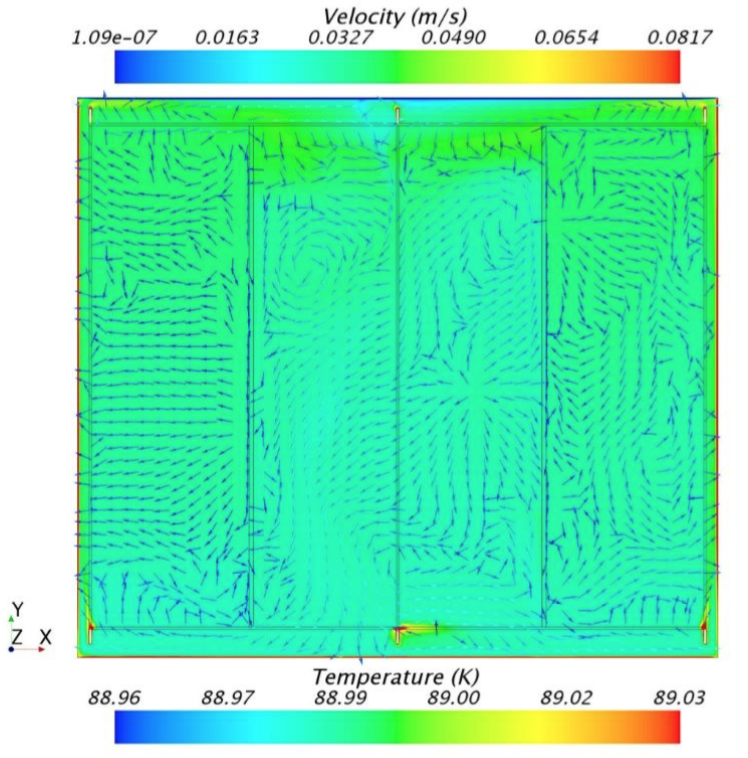
\includegraphics[height=0.4\textwidth]{cisc_cfd_outlet_z0.png}
  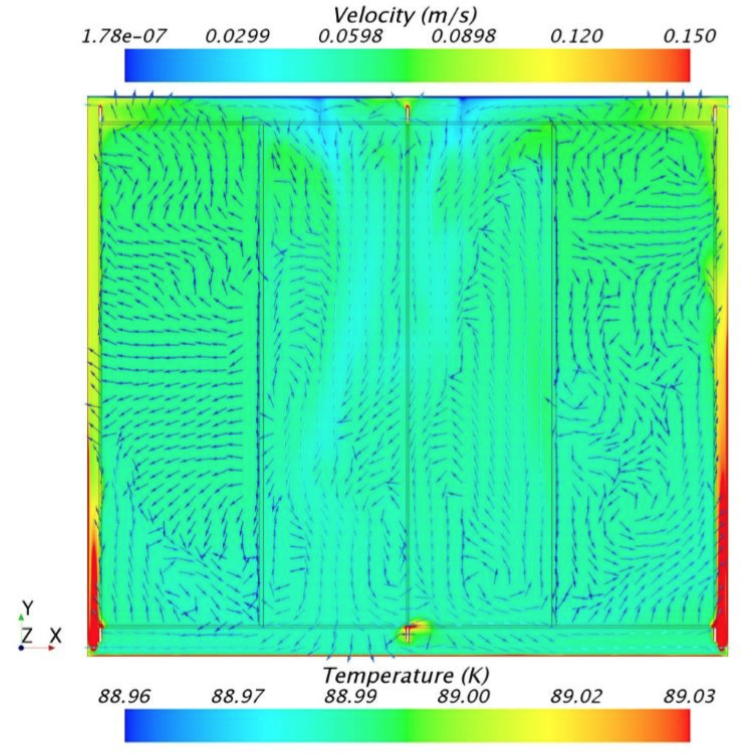
\includegraphics[height=0.4\textwidth]{cisc_cfd_inlet_z52.png}
\end{dunefigure}

Fig.~\ref{fig:cfd-example} shows an example of the temperature
distribution on a plane intersecting a \dword{lar} inlet and at a
plane halfway between an inlet and an outlet; 
the geometry used for
this simulation is shown in Fig.~\ref{fig:cfd-example-geometry}. Note the plume of higher temperature \dword{lar} between the walls and
the outer APA on the inlet plane. The current placement of instrumentation in
the cryostat as shown in Fig.~\ref{fig:cisc-tsensor-map} was determined using temperature and impurity distributions from previous simulations.

\begin{dunefigure}[\dword{cisc} geometry layout]{fig:cfd-example-geometry}
  {Layout of the \dword{tpc} within the cryostat (top) and positions of \dword{lar} inlets and outlets (bottom) as modeled in the SDSU \dword{cfd} simulations~\cite{docdb-5915}. The Y axis is vertical and the X axis is parallel to the \dword{tpc} drift direction. Inlets are shown in green and outlets are shown in red.}
  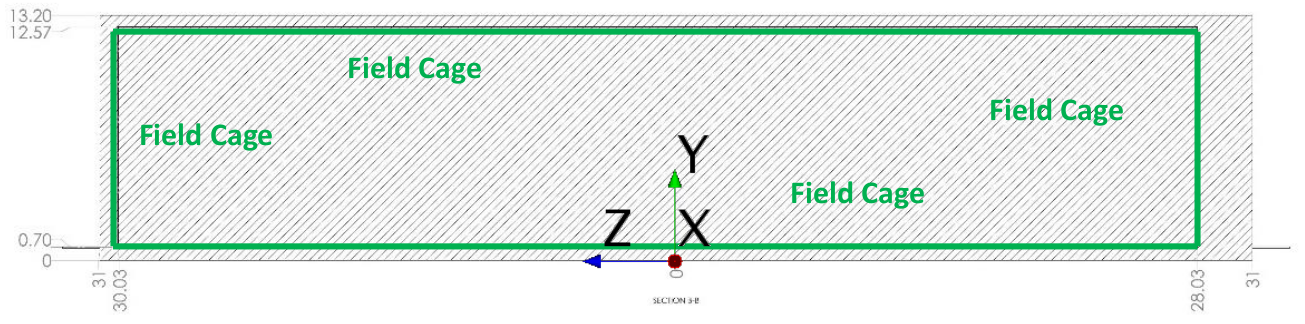
\includegraphics[width=0.7\textwidth]{cisc_cfd_cryostat-layout.png}
  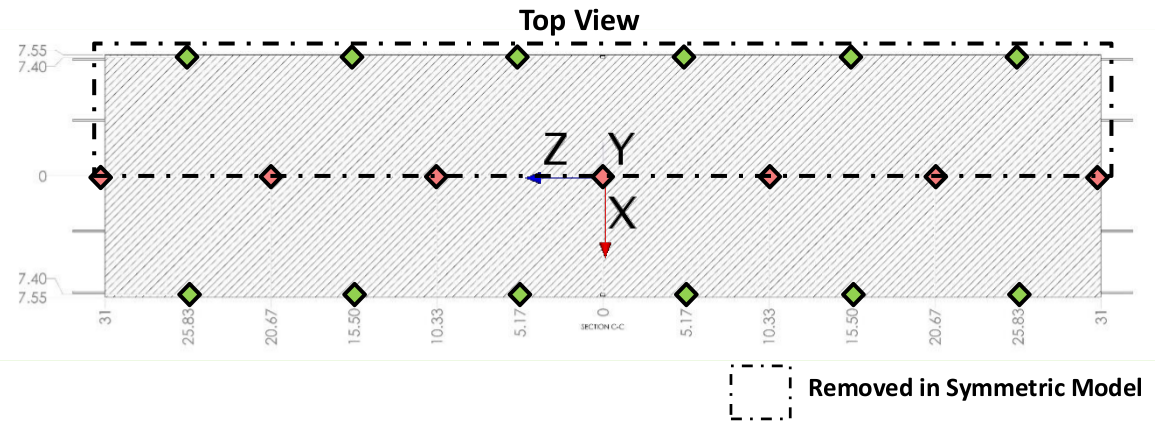
\includegraphics[width=0.7\textwidth]{cisc_cfd_inlet-outlet-layout.png}
\end{dunefigure}

The strategy for the future \dword{cfd} simulations begins with understanding the performance of the ProtoDUNE-SP cryogenics system and modeling the far detectors to derive requirements for instrumentation. The following is a prioritized set of studies planned (some currently underway) to help determine the requirements for other systems:
\begin{itemize}
\item Review the \dword{dune} \dword{fd} cryogenics system design and verify the current implementation in simulation to ensure that the model represents what will be built.
\item 
Model the ProtoDUNE-SP liquid and gas regions with the same precision as the \dword{fd}. Presently, we have only the liquid model, which is needed to interpret the thermometer data. The gas model is needed to see how to place thermometers in the ullage and verify the design of the gaseous argon purge system.
% \item Perform a \dword{cfd} study to determine the feasibility of a wier for DP; this helps to determine if it can be used to clean the \dword{lar} surface before the extraction grid is submerged in the DP module.
\item Verify the SP \dword{cfd} model for the \dword{fd} SP module in simulation performed by LBNF; this defines the requirements for instrumentation devices (e.g., thermometry).
% \item Model the ProtoDUNE-DP liquid and gas regions with the same precision as the \dword{fd}.
\end{itemize}

\begin{dunetable}
[CFD parameters for \dword{protodune}]
{p{0.25\textwidth}p{0.15\textwidth}p{0.5\textwidth}}
{tab:fdgen-cisc-CFDparam}
{CFD input parameters for \dword{protodune}}   


Parameter  &	Value &	Comments \\ \toprowrule
Cryostat height
&
7.878 m
&
Measured with laser (1 cm error approx.)
\\ \toprowrule	
LAr surface height
&
7.406 m
&
Measured by capacitive level meter ($<1$ cm error)
\\ \toprowrule	
Ullage pressure		
&
1.045 bar
&
Measured by pressure gauges
\\ \toprowrule
LAr surface temperature
&
87.596 K
&
computed using ullage pressure and \linebreak
https://lar.bnl.gov/properties/basic.html\#phase
\\ \toprowrule
LAr inlet temperature
&
outlet + 0.2 K
&
Estimated
\\ \toprowrule
LAr flow rate per pipe
&
0.4170025 kg/s
&
\\ \toprowrule		
Heat flux 
&
5.76 $W/m^2$		
&
This is the Heat flux from all four walls as well as the ground
\\ \toprowrule
Vapor being drawn from the chimneys
&
5-7 gr/sec
&
among all chimneys
\\
\end{dunetable}

\subsection{Validation in ProtoDUNE}

We can collect data at ProtoDUNE-SP to validate \dword{cfd} using already installed instrumentation:
\begin{itemize}
\item Static and dynamic T-gradient thermometers
\item Individual temperature sensors placed in the return \dword{lar} inlets
\item Two 2D grids of individual temperature sensors installed below the bottom ground planes and above the top ground planes
\item A string of three purity monitors vertically spaced from near the bottom of the cryostat to just below the \dword{lar} surface
\item H$_{2}$O, N$_{2}$, and O$_{2}$ Gas analyzers
\item \dword{lar} level monitors
\item Standard cryogenic sensors like pressure transducers, various individual temperature sensors placed around
the cryostat on the membrane walls, and recirculation flow rates transducers
\end{itemize}

\fixme{I notice the list format here is somewhat different from other chapters. We may need to go through and make punctuation at the end of each item and at the end of the list consistent throughout the manuscript.}

These devices are running and have already produced data logged through slow controls and available for offline analysis.

The temperature profiles of the ProtoDUNE-SP \fixme{Abbreviation format?} simulation are being compared with experimental temperature probe data. This work is ongoing, but we have preliminary results. Fig.~\ref{fig:cisc-cfd-valid} shows the fluid temperature measured by the temperature probe and compares it with the current ProtoDUNE-SP \dword{cfd} model with parameters shown in Table \ref{tab:fdgen-cisc-CFDparam}.\todo{Confirm this table is referenced correctly as input parameters to the iteration procedure for comparison with temperature probes.} 
The validation procedure consists of an iterative process where several versions of the \dword{cfd} simulations, with using different input parameters, have been produced to converge on a reasonable agreement. \fixme{To me, this does not appear to have sufficient detail to be clear.}

\begin{dunefigure}[Comparison of ProtoDUNE-SP temperature data and CFD simulations]{fig:cisc-cfd-valid}
  {Comparison of ProtoDUNE-SP temperature data and CFD simulations.}
  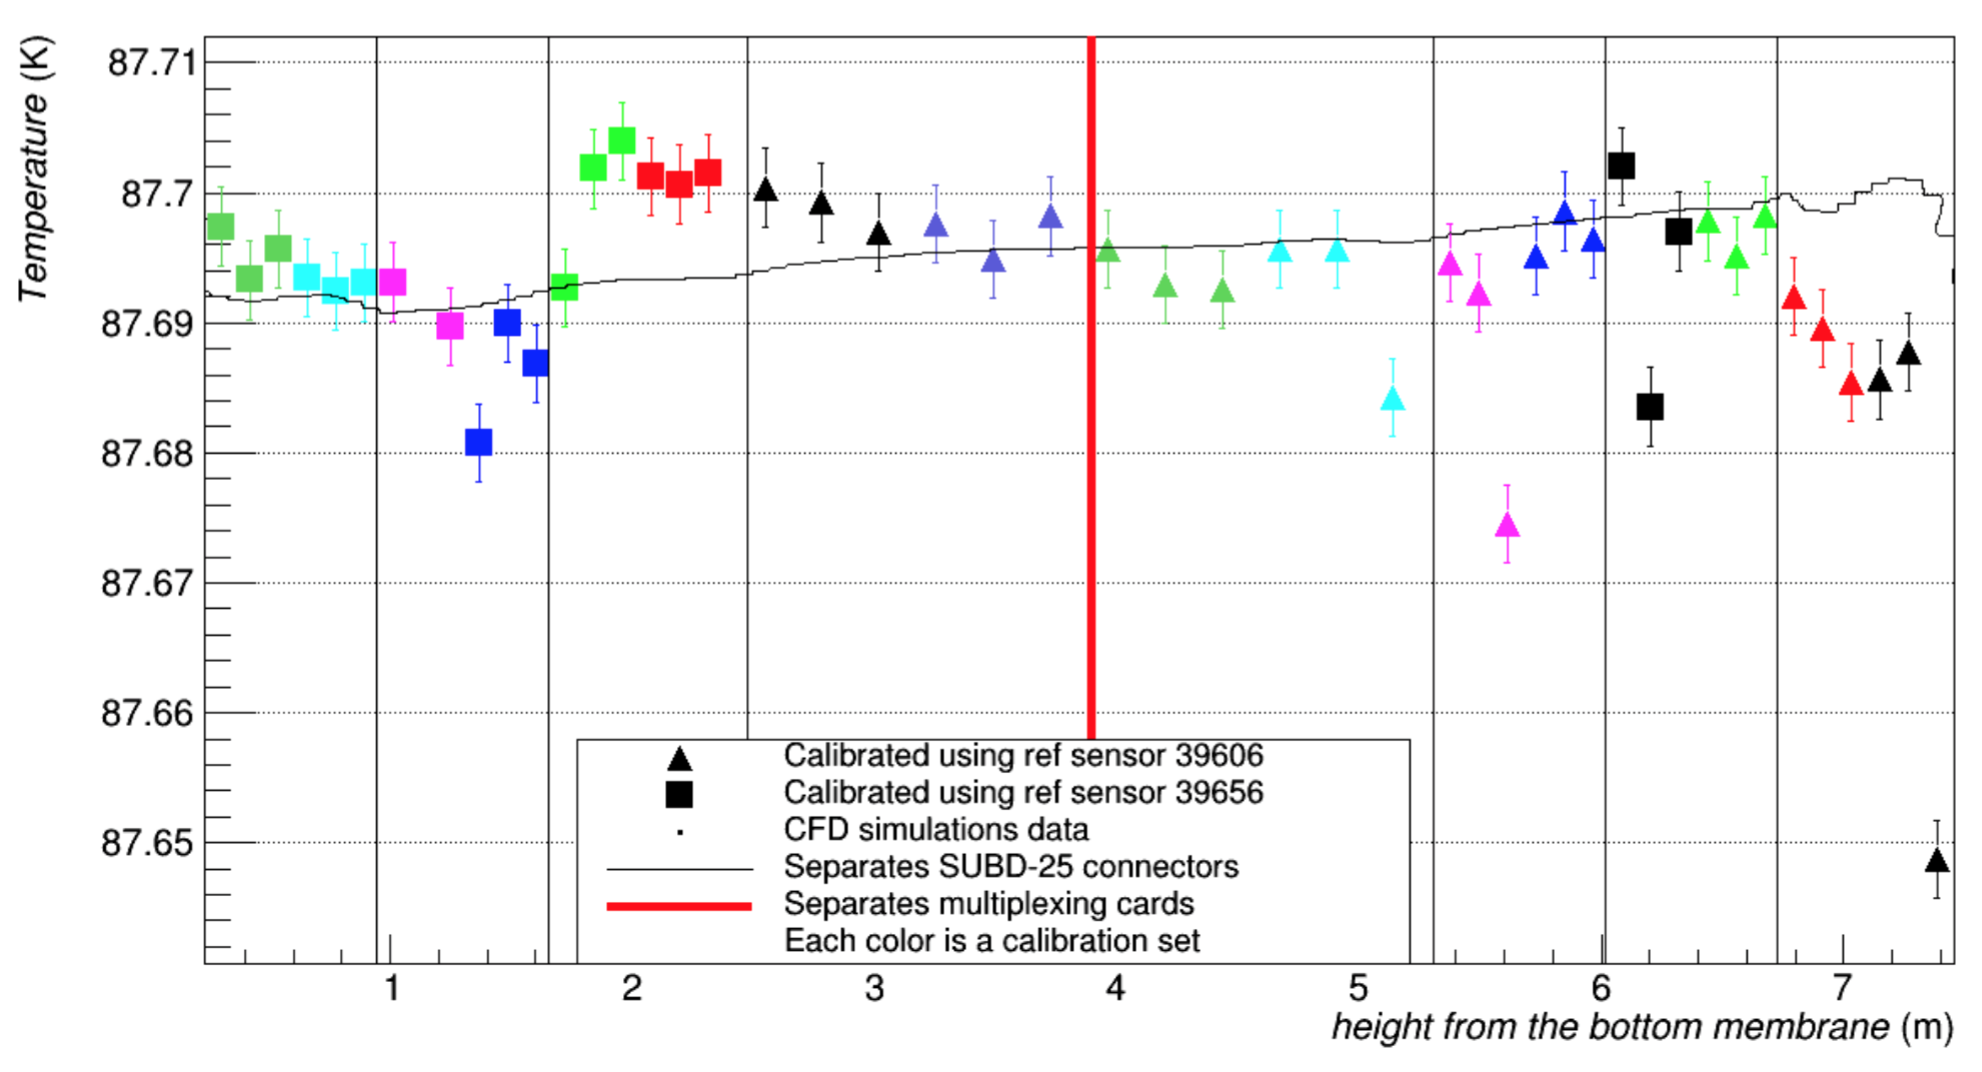
\includegraphics[width=0.6\textwidth]{cisc_CFD_valid_v0.png}
\end{dunefigure}

After further refining, the \dword{cfd} models should provide additional data from purity monitors to compare with the results to see that the simulations can accurately map impurity levels in the detector. Streamlines\footnote{In fluid mechanics, a streamline is a line that is everywhere tangent to the local velocity vector. For steady flows, a streamline also represents the path that a single particle of the fluid will take from inlet to exit.} from the current ProtoDUNE-SP simulation (Fig.~\ref{fig:cisc-cfd-larflow-inlets}) show the flow paths from the four inlets to the outlet of the cryostat.

\begin{dunefigure}[lar flow inlets]{fig:cisc-cfd-larflow-inlets}
  {Streamlines for liquid argon flow inside the ProtoDUNE-SP detector.}
  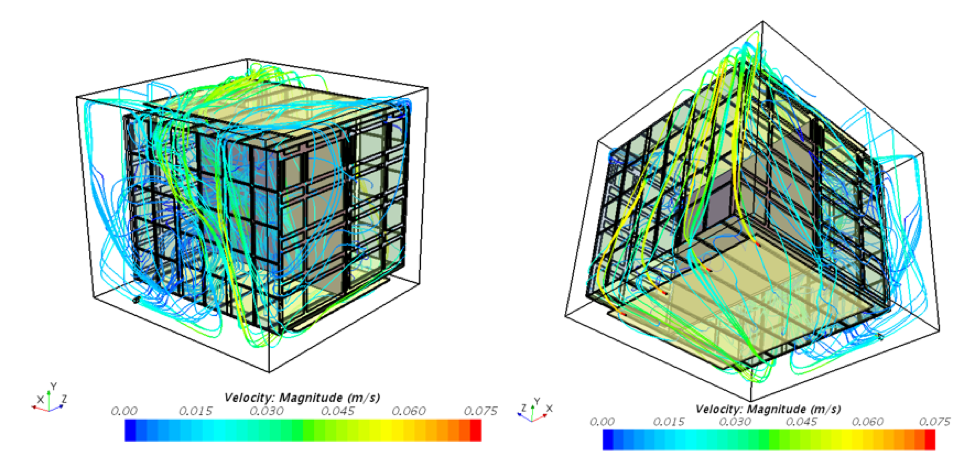
\includegraphics[width=0.8\textwidth]{cisc_cfd_larflow-inlets.png}
\end{dunefigure}

Additional dedicated tests are also planned to validate \dword{cfd} provoking changes to the cryostat environment; measuring the instrumentation response may help establish the validity of the \dword{cfd} model. The \dword{cfd} predicts a reasonable response for more than one set of initial conditions, which is reassuring. For these additional tests, we can reasonably wait until the beam run is finished because they \fixme{They who?} could have undesirable effects on the cryostat environment. Some possible additional tests include pump/recirculation manipulations such as pump on/off, pumping speed change, and bypassing filtration. Additionally, changes in the pressure can be induced by setting the cryostat pressure set point to a higher (or lower) value\footnote{The HV could be ramped down for this exercise because dropping the pressure too fast might provoke boiling of the LAr near the
surface.} \fixme{In the footnote, another abbreviation to be fixed?} for a specified time while monitoring the instrumentation. Any change in pressure could change the temperatures everywhere in the cryostat. Studying the rate of this change, as
detected in the various vertical heights of the cryostat, might provide interesting constraints on the \dword{cfd} model. 

%\fixme{The plan is to PRODUCE A NEW MAP WITH THE HAWAII DATA INCLUDED AND THE NEW CFD SIMULATION, BY THE END OF DECEMBER. Text will be updated accordingly to discuss new results.}

%%%%%%%%
\section{Cryogenic Instrumentation}
\label{sec:fdgen-cryo-instr}
Instrumentation inside the cryostat must ensure that the condition of the \dword{lar} is adequate to operate the \dshort{tpc}.
This instrumentation includes devices (the purity monitors) to check the level of impurity in the argon and providing high-precision electron lifetime measurements,
as well as gas analyzers to ensure that the levels of atmospheric contamination drop below certain limits during the cryostat purging, cooling, and filling.
The cryogenics system operation is monitored by temperature sensors deployed in vertical arrays and at the top and bottom of the detector, providing a 
detailed \threed temperature map that helps predict the \dword{lar} purity across the entire cryostat. The cryogenics instrumentation also includes \lar level monitors and
a system of internal cameras to help find sparks in the cryostat and for overall monitoring of the cryostat interior. 

%Reference to CFD (lo que esta escrito no vale, es un primer intento copiando la introduccion de la seccion CFD)
As mentioned in previous section \fixme{The section should be identified by number.} , fluid motion within the cryostat must be simulated using a \dfirst{cfd} code.
The proper placement of purity monitors, thermometers, and liquid level monitors in the \dword{detmodule} requires knowing how \dword{lar} behaves within the cryostat in terms of its fluid dynamics, heat and mass transfer, and distribution of impurity concentrations. Besides that, to coherently analyze the instrumentation data requires the results of such simulations.

%Something on ProtoDUNE Validation 
The performance of all cryogenic instrumentation for DUNE-FD \fixme{An abbreviation problem?} is being tested in ProtoDUNE-SP \fixme{And another abbreviation problem?} , validating the baseline design for DUNE-FD.

%%%%%%%%%%%%%%%%%%%%%%%%%%%%%%%%%%%%%%%%%%%%%%%%%%%%%%
%%%%%%%%%%%%%%%%%  PURITY MONITORS %%%%%%%%%%%%%%%%%%%

%%%%%%%%%%%%%%%%%%%%%%%%%%%%%%%%%%%

\subsection{Purity Monitors}
\label{sec:fdgen-slow-cryo-purity-mon}

%Laura, Jianming
A fundamental requirement of a \dword{lar} \dshort{tpc} is that ionization electrons drift over long distances in \dword{lar}. Part of the charge is inevitably lost because of electronegative impurities in the liquid. To keep this loss to a minimum, monitoring impurities and purifying the \dword{lar} during operation is essential.




A purity monitor is a small ionization chamber used to independently  infer the effective free electron lifetime in the \lartpc.  The operating principle of the purity monitor consists of generating a known electron current by illuminating a cathode with UV \fixme{This abbreviation may be so commonly used that defining it is not necessary.} light, then at an anode, collecting  the current that survives after drifting a known distance.  Attenuation of the current is related to the lifetime of the electron.
Electron loss can be parameterized as
%
\(N(t) = N(0)e^{-t/\tau},\)
%
where $N(0)$ is the number of electrons generated by ionization, $N(t)$ is the number of electrons after drift time $t$, and $\tau$ is the electron lifetime. 

For the \dword{spmod}, the drift distance is \spmaxdrift, and the \efield is \SI{500}{\volt\per\centi\meter}. Given the drift velocity of approximately \SI{1.5}{\milli\meter\per\micro\second} in this field, the time to go from cathode to anode is around \SI{\sim2.4}{\milli\second} \cite{Walkowiak:2000wf}.
The \dword{lar} \dshort{tpc} signal attenuation, \([N(0)-N(t)]/N(0)\), must be kept less than \SI{20}{\percent} over the entire drift distance \cite{fdtf-final-report}. The corresponding electron lifetime is $2.4/[-\ln(0.8)] \simeq \SI{11}{ms}$.
% (The corresponding \dword{lar} O2 purity requirement is about \SI{30}{ppt}.)

Residual gas analyzers are an obvious choice when analyzing argon gas and can be used to monitor the gas in the ullage of the tank. Unfortunately, suitable, commercially available  mass spectrometers have a detection limit of \num{\sim10}\dword{ppb}, whereas DUNE requires a sensitivity of \dword{ppt}. Therefore, specially constructed purity monitors measure \lar purity in all the phases of operation, enabling the position-dependent purity measurements needed to achieve DUNE's \fixme{abbreviation} physics goal. 
%Purity monitors also have the potential to be developed as a calibration tool that provides high precision and real-time electron lifetime measurements for wire-by-wire detector calibration.

Purity monitors also serve to mitigate the risk of \lar contamination.  The large scale of the \dwords{detmodule} increases the risk of failing to notice a sudden unexpected infusion of contaminated \lar being injected back into the cryostat.   
If this condition were to persist, it could cause irreversible contamination to the \dword{lar} and terminate useful data taking.  Strategically placed purity monitors mitigate this risk; the purity monitors installed in the \dword{pdsp} detector demonstrate this.

Purity monitors are placed inside the cryostat but outside of the detector \dshort{tpc}, as well as outside the cryostat within the recirculation system before and after filtration. 
Continuous monitoring of  the \dword{lar} supply lines to the \dword{detmodule} provides a strong line of defense against contaminated \lar. Gas analyzers (described in Section~\ref{sec:fdgen-slow-cryo-gas-anlyz}) provide a first line of defense against contaminated gas.  Purity monitors inside the \dword{detmodule} provide critical defense against liquid argon contamination caused by pump and filter problems, as well as all sources of contamination in the \lar volume and contamination from recirculated \lar. 

Furthermore, using several purity monitors to measure lifetime with high precision at carefully chosen points provides key input, like vertical gradients in impurity concentrations, for \dshort{cfd} models of the detector.

Purity monitors were deployed in previous LArTPC experiments: ICARUS, \microboone, and \dword{35t}. During the first run of the \dword{35t}, two of the four purity monitors stopped working during cooldown, and a third operated intermittently. We later found that this was due to poor electrical contacts between the resistor chain and the purity monitor. A new design was implemented and successfully tested in the second run. 


The \dword{pdsp} and \dword{pddp} use purity monitoring systems consisting of several purity monitors that measure electron lifetime at different heights. Figure~\ref{fig-pdsp-prmassembly} shows the assembly of the ProtoDUNE-SP \fixme{abbreviation} purity monitors. The design was changed to ensure electric connectivity and improve signals. \dword{pdsp} uses a string of purity monitors connected with stainless steel tubes to protect the optic fibers. The purity monitor system at \dword{pdsp} measured electron lifetime on a hours base \fixme{every hour instead of on an hours base?} during commissioning and daily during the beam test. During commissioning and while running the test beam, the purity monitor system at \dword{pdsp} alerted us to serious problems twice. The first time was for filter saturation, and the second was that the recirculation pump had stopped. Those alerts were crucial to the success of running the test beam in the \dword{pdsp} project by preventing situations that otherwise would have had serious consequences for taking any beam data if they had continued unnoticed.

\begin{dunefigure}[The ProtoDUNE-SP purity monitoring system]{fig-pdsp-prmassembly}
  {The ProtoDUNE-SP purity monitoring system}
  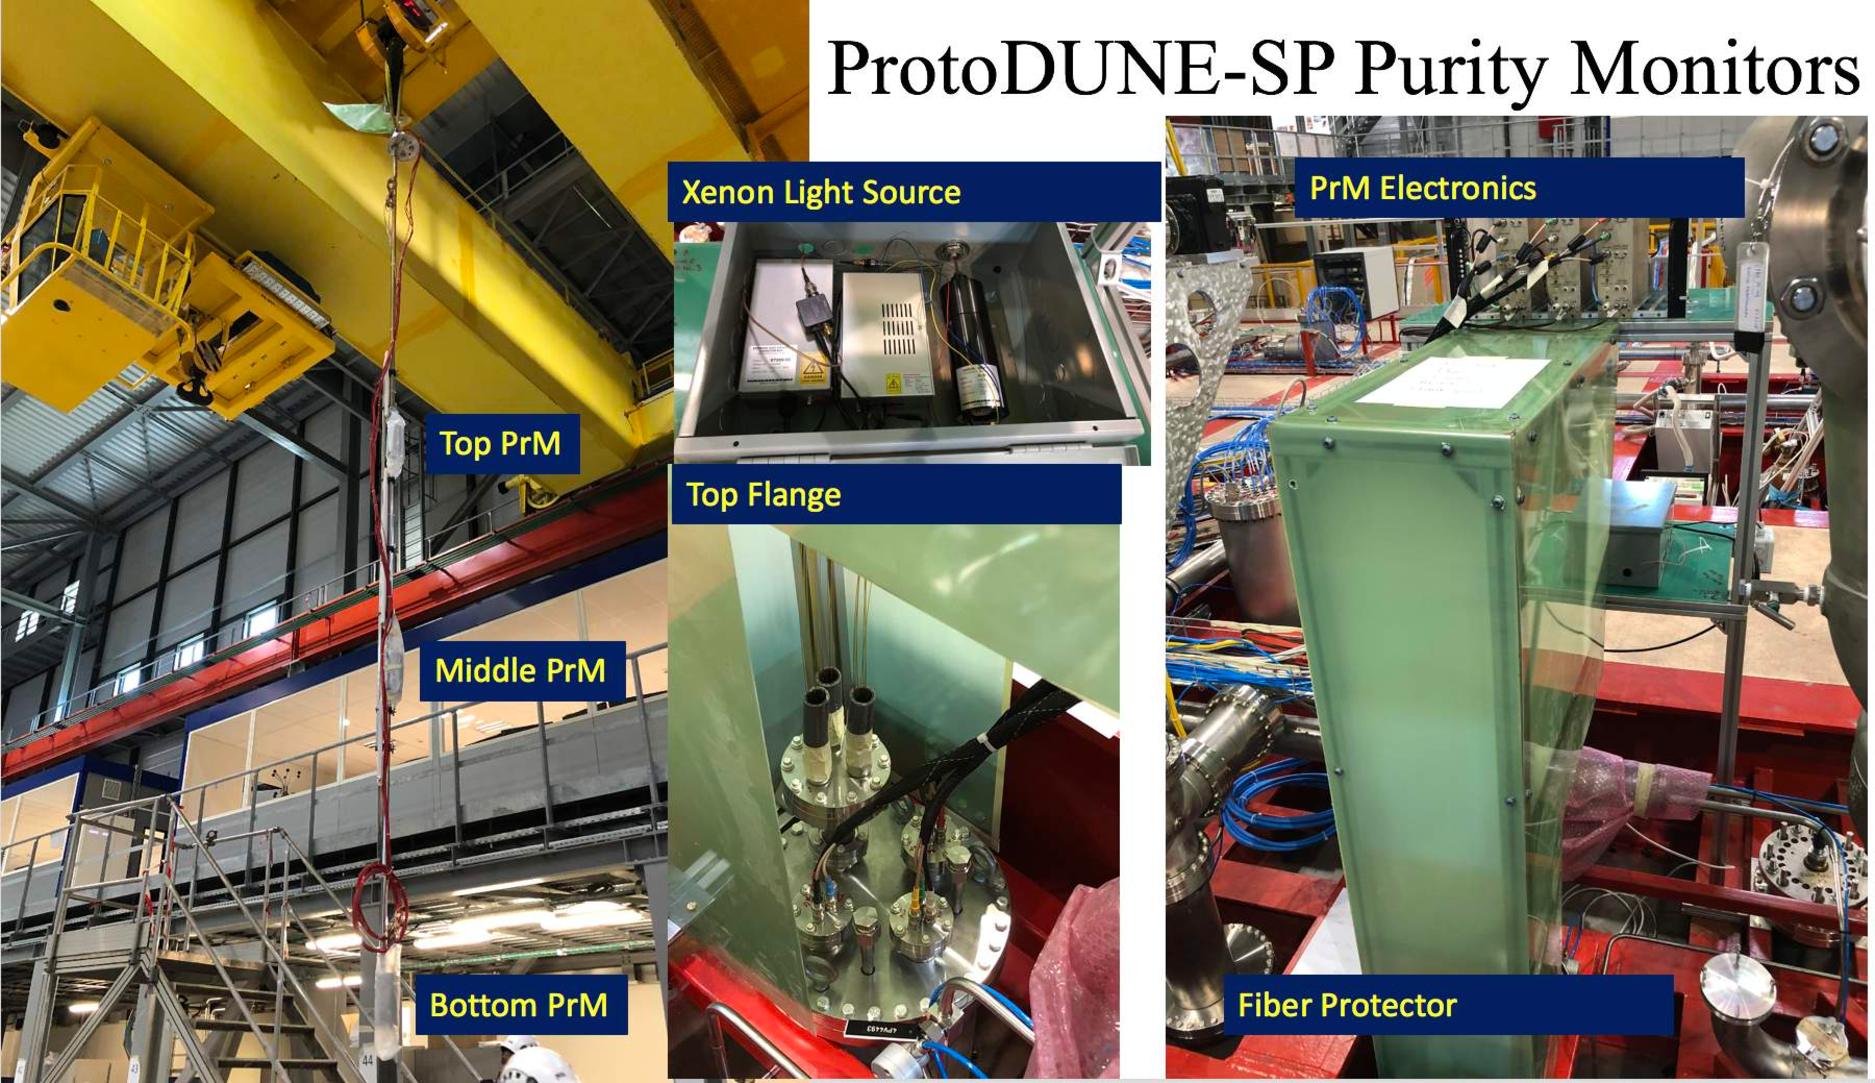
\includegraphics[width=0.9\textwidth]{PrMon_pdsp-PrMAssembly.pdf}
\end{dunefigure}



The \dword{pdsp}  purity monitors operated with different high voltages to change electron drift time, which then ranged from 150 $\mu$s to 3 ms. This allowed the \dword{pdsp} purity monitors to measure electron lifetime from 35 $\mu$s to about 10 ms with high precision. In other words, the purity monitors can measure lifetimes over a dynamic range higher than 300. This high precision electron lifetime measurement was also valuable to the lifetime calibration for  \dword{pdsp}. Because purity monitors have much small drifter \fixme{Should this be "drift"?} volumes than the \dshort{tpc}, they are less affected by the space charge caused by cosmic rays. 

  A similar purity monitoring system design and operation plan are exploited in the DUNE \fixme{abbreviation} \dword{fd}, with modifications to accommodate the instrumentation port placement relative to the purity monitor system and the requirements and constraints of different geometric relationships between the \dshort{tpc} and cryostat.




%%%%%%%%%%%%%%%%%%%%%%%%%%%%%%%%%%%%%%%%%%
%\subsubsection{Physics and Simulation}
% Andrew, Jianming





The \dword{pdsp} at CERN had three purity monitors. Figure~\ref{fig-pdsp-prm} shows the data taken using them between the commissioning of \dword{pdsp} in September, 2018, to the middle of test beam running, November, 2018. 

\begin{dunefigure}[The measured electron lifetimes in the four purity monitors as a function of time at ProtoDUNE-SP prototype]{fig-pdsp-prm}
  {The measured electron lifetimes in the four purity monitors as a function of time in the ProtoDUNE-SP prototype.}
  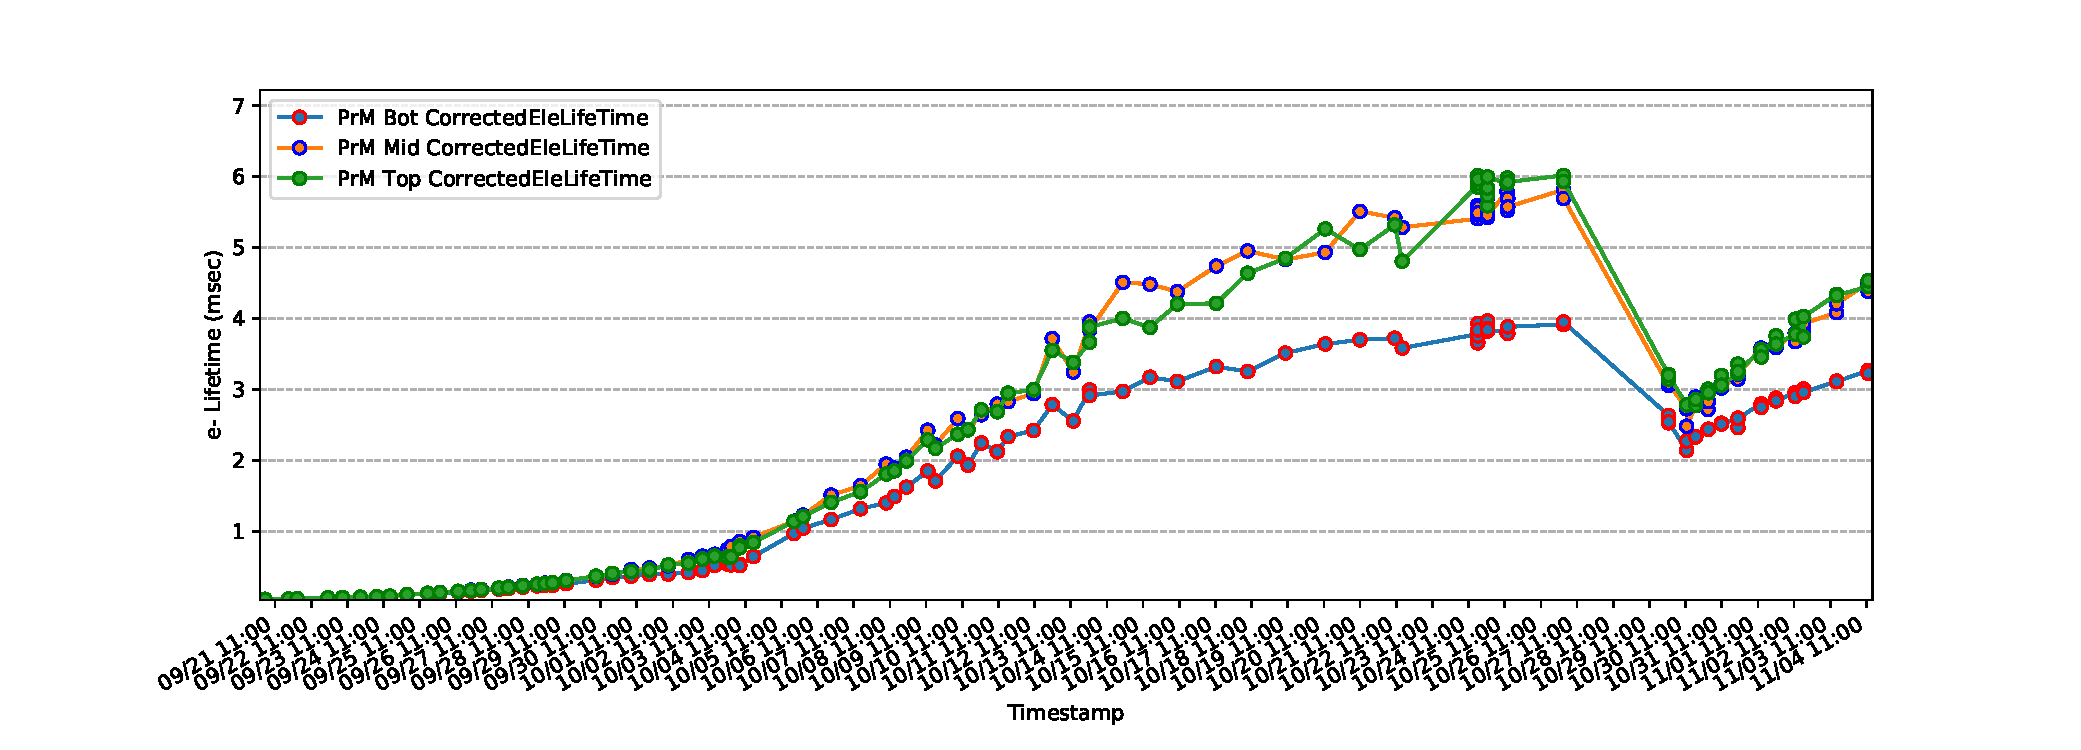
\includegraphics[width=0.9\textwidth]{PrMon_pdsp-PrM.pdf}
\end{dunefigure}




%%%%%%%%%%%%%%%%%%%%%%%%%%%%%%%%%%%%%%%%%
\subsubsection{Purity Monitor Design}
%Laura, Jianming
%WIP IF YOU HAVE MIP PARTICLES LIKE MUONS... NOT TRUE WHEN YOU ARE UNDERGROUND. ALSO, WE HAVE SEEN IN THE 311 THAT MUONS DO NOT DEPOSIT THE EXACT SAME AMOUNT OF ENERGY ACROSS THE TRACK 
%While the \dword{lar} \dshort{tpc} itself can measure the purity of the liquid argon based on the drift electron lifetime, this can only be done once a certain level of purity has been achieved, and until then it may be unclear what the level of purity is and if conditions in the detector are becoming better or worse. 

The basic design of a purity monitor uses the design in the ICARUS experiment (Figure~\ref{fig:prm})\cite{Adamowski:2014daa}: a double-gridded ion chamber immersed in the \lar volume.   The purity monitor has four parallel, circular electrodes, a disk holding a photocathode, two grid rings (anode and cathode), and an anode disk. The cathode grid is held at ground potential. The cathode, anode grid, and anode are electrically accessible via modified vacuum grade high-voltage \fdth{}s and separate bias voltages held at each one.  
The anode grid and the field shaping rings are connected to the cathode grid by an internal chain of \SI{50}{\mega\ohm} resistors to ensure the uniformity of the \efield{}s in the drift regions. A stainless mesh cylinder is used as a Faraday cage to isolate the purity monitor from external electrostatic background. 

The purity monitor measures the electron drift lifetime between its anode and cathode. The electrons are generated by the purity monitor's UV-illuminated gold photocathode via the photoelectric effect. Because the electron lifetime in \lar is inversely proportional to the electronegative impurity concentration, the fraction of electrons generated at the cathode that arrive at the anode ($Q_A/Q_C$) after the electron drift time $t$ gives a measure of the electron lifetime $\tau$:
%
\( Q_A/Q_C \sim e^{-t/\tau}.\)



\begin{dunefigure}[Schematic diagram of the basic purity monitor design]{fig:prm}
  {Schematic diagram of the basic purity monitor design \cite{Adamowski:2014daa}.}
  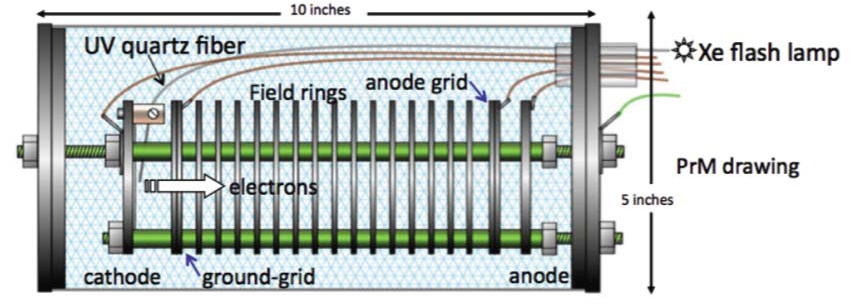
\includegraphics[width=0.9\textwidth]{PrMon_prm.pdf}
\end{dunefigure}


%
%Complete formula would be: Q_A/Q_C = \frac{T_1 \sinh(t_3/2\tau)}{t_3 \sinh(t_1/2\tau)} \exp \left(-\frac{t_2+\frac{t_1+t_3}{2}}{\tau} \right), where$t_1$ is the time it takes the electrons to go from cathode to cathode grid, $t_2$ to go from cathode grid to anode grid, and $t_3$ to go from grid anode to anode. 

This formula shows the purity monitor reaches its sensitivity limit once the electron lifetime becomes much larger than the drift time $t$. For $\tau >> t$, the anode to cathode charge ratio becomes $\sim\,1$, but, because the drift time is inversely proportional to the \efield, lowering the drift field means, in principle, any lifetime can be measured no matter the length of the purity monitor (the lower the field, the lower the drift velocity, i.e., the longer the drift time). On the other hand, increasing the voltage will shorten the drift time, allowing purity monitors to measure a short lifetime when purity is low. 

According to our experience with \dword{pdsp}, for a 9.5-inch-long purity monitor, varying the operational high voltage on the anode from 250 V to 4000 V allows the purity monitors to measure an electron lifetime ranging from 35 $\mu$s to approximately 10 ms with high precision. 

In practice, at very low fields, drifting the electrons all the way up to the anode is difficult, and the discharge in the gas phase limits the anode high voltage to go above 4000 V. \fixme{I read this as "the discharge in the gas phase keeps the voltage in the anode below 4000V." Is that correct?}

The electron lifetime of the purest commercial liquid argon after the first filtering during the filling process is typically higher than 40$\mu$s. However, when the filter starts to saturate, the lifetime will be less than 30 $\mu$s.  To achieve less energy loss due to impurity,  the DUNE \dword{fd} requires the electron lifetime to be more than 10 ms. Therefore, purity monitors with different lengths (drift distances) are needed to extend the measuring range of purity lower than 35 $\mu$s and higher than 10 ms.
%Currently, specific sensitivity limits for purity monitors with a drift distance of the order of $\sim$\SI{20}{\centi\meter} are still to be determined in a series of tests. If the required sensitivity is not achieved by these ``short'' purity monitors, longer ones may be developed.

The photocathode that produces the \phel{}s is an aluminum plate coated with \SI{50}{\angstrom} of titanium and \SI{1000}{\angstrom} of gold and attached to the cathode disk. A xenon flash lamp is the light source in the baseline design, although this could be replaced by a more reliable and possibly submersible light source in the future, perhaps LED driven. The UV output of the lamp is quite good, approximately $\lambda=$ \SI{225}{\nano\meter}, which is close to the work function of gold (\SIrange{4.9}{5.1}{\eV}). Several UV quartz fibers carry the xenon UV light into the cryostat to illuminate the gold photocathode.   Another quartz fiber delivers the light into a properly biased photodiode outside the cryostat to provide the trigger signal when the lamp flashes. 



\subsubsection{Electronics, DAQ, and Slow Controls Interfacing}
%Jianming
The purity monitor electronics and \dword{daq} system consist of \dword{fe} electronics, waveform digitizers, and a \dword{daq} PC.  Figure~\ref{fig:cryo-purity-mon-diag} shows the block diagram of the system.


\begin{dunefigure}[Block diagram of the purity monitor system.]{fig:cryo-purity-mon-diag}
  {Block diagram of the purity monitor system.}
  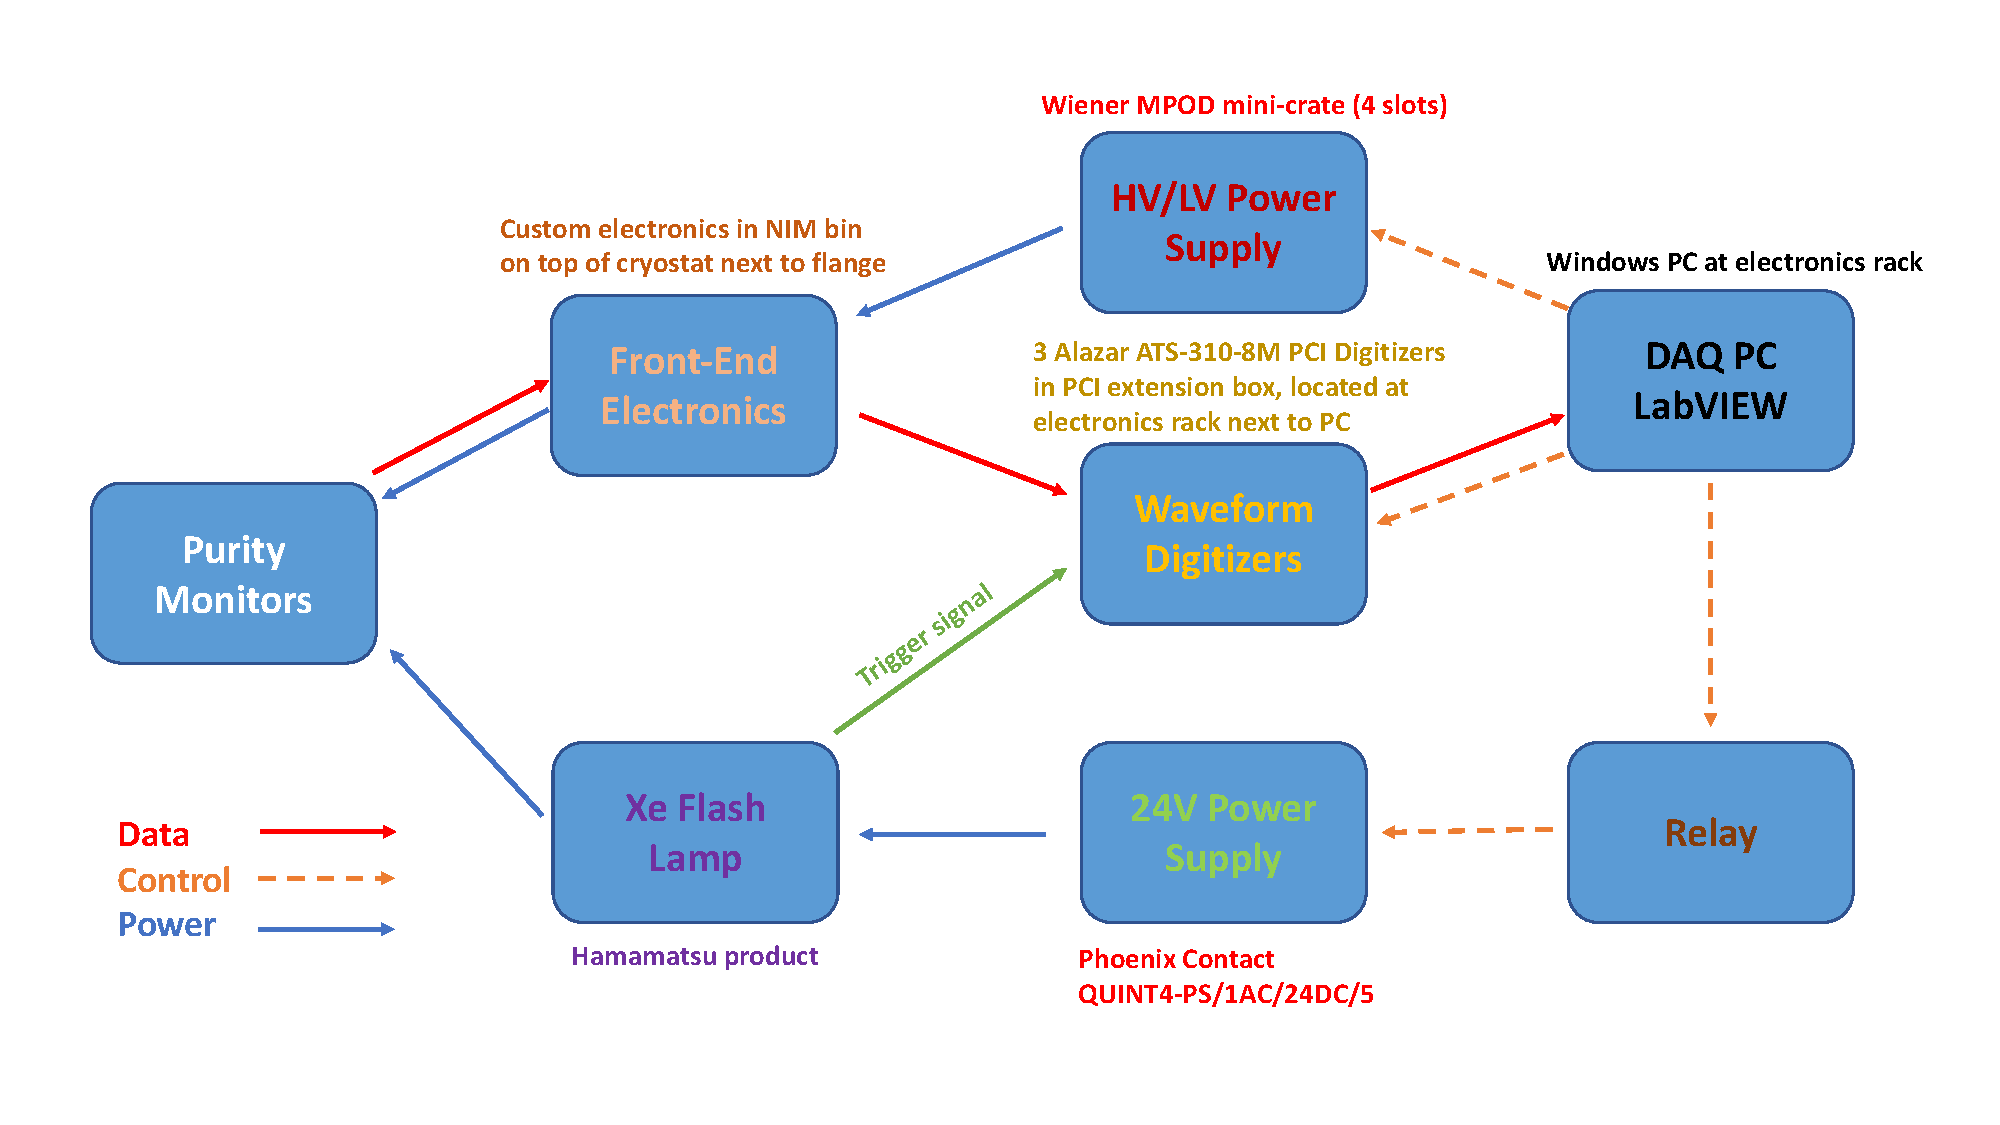
\includegraphics[width=0.9\textwidth]{PrMon_BlockDiagram.pdf}
\end{dunefigure}


The baseline design of the \dword{fe} electronics is the one used for the purity monitors for the \dword{35t}, LAPD, and \microboone. The cathode and anode signals are fed into two charge amplifiers contained within the purity monitor electronics module.
This electronics module includes a HV filter circuit and an amplifier circuit, both shielded by copper plates, so the signal and high voltage can be carried on the same cable and decoupled inside the purity monitor electronics module.
The amplified outputs of the anode and cathode are recorded using a waveform digitizer that interfaces with a \dword{daq} PC.
The shields of the signal and HV cable connect to the grounding points of the cryostat and are separated from the electronic ground with a resistor and a capacitor connected in parallel, mitigating ground loops between the cryostat and the electronics racks. Amplified output is transmitted to an AlazarTech ATS310 waveform digitizer containing two input channels, each with 12-bit resolution. Each channel can sample a signal at a rate of \SI{20}{\mega\samples\per\second} to \SI{1}{\kilo\samples\per\second} and storing up to \SI{8}{\mega\samples} in memory. One digitizer is used for each purity monitor, and each \fixme{Digitizer or purity monitor?} interfaces with the DAQ PC across the PCI bus. 

A custom LabVIEW application running on the \dword{daq} PC has two functions: it controls the waveform digitizers and the power supplies, and it monitors the signals and key parameters. The application configures the digitizers to set the sampling rate, the number of waveforms to be stored in memory, pre-trigger data, and a trigger mode. A signal from a photodiode triggered by the xenon flash lamp is fed directly into the digitizer as an external trigger to initiate data acquisition. The LabVIEW application automatically turns on the xenon flash lamp by powering a relay when data taking begins and then turns it off when finished.
The waveforms stored in the digitizers are transferred to the DAQ PC and used to obtain averaged waveforms to reduce the electronic noise in the waveforms. The baseline is estimated using the pre-trigger data and subtracted from the waveforms \fixme{I read this as "...is estimated by subtracting the pre-trigger date from the waveforms..." Is that correct? If so, then use the revised text. If not, this needs some other revision to make it clear.} to measure peak voltages of the cathode and anode signals. These processes are performed in real time within the application and are then used to estimate the electron lifetime.
The application continuously displays the waveforms and important parameters like measured electron lifetime, peak voltages, and drift time of electrons in the purity monitors and shows these parameters over time.
This allows validating the impurity of the \dword{lar} and seeing effects that may not be spotted at that instant. Instead of storing the measured parameters, the waveforms and the digitizer configurations are recorded in binary form for offline analysis. ISEG HV modules in a WIENER MPOD mini crate supply negative voltages to the cathode and positive voltages to the anode. The LabVIEW application controls and monitors the HV systems through an Ethernet interface.  \fixme{Check the tenses. I see some past tense, quite a lot of present tense, and then some future tense. Make sure tense matches when something occurs, has occurred, or will occur.}

The xenon flash lamp and the \dword{fe} electronics are installed close to the purity monitor flange, to reduce light loss through the optical fiber and prevent signal loss. Other pieces of equipment are mounted in a rack separate from the cryostat. They distribute power to the xenon flash lamp and the \dword{fe} electronics and collect data from the electronics. The slow control system communicates with the purity monitor \dword{daq} software and controls  the \dword{hv} and \dword{lv} power supplies of the purity monitor system. The optical fiber must be very close to the photocathode (less than \SI{0.5}{\milli\meter}) for efficient \phel extraction, so little interference with the \dword{pds} is expected. \fixme{I read the following sentence and had some trouble untangling the series of prepositional phrases. Is this what you mean? "The electronics of purity monitors could induce noise in the TPC electronics; this usually occurs when the xenon light source in the purity monitor produces a flash, creating discharge from the main capacitor of the purity monitor."}
The electronics of purity monitors could induce noise in the \dshort{tpc} electronics, largely from the current surge in the discharging process of the main capacitor of the purity monitor xenon light source when producing a flash.  This source of noise can be controlled by placing the xenon flash lamp inside its own Faraday cage, which allows proper grounding and shielding; the extent of mitigation will be evaluated at \dword{protodune}. According to the operation of purity monitors at \dword{pdsp}, after careful checks of the grounding, this noise is well below noise generated by other sources.

We will use triggering to prevent any potential noise from the purity monitor's flash lamp from affecting TPC and \dword{pds} signals. The neutrino spill trigger rate is a few hertz, and each trigger window is one or a few milliseconds. For a purity monitor's flash lamp,  the flash light pulse is very short (a microsecond or so, much shorter than the gaps between LArTPC trigger windows). Thus, a LArTPC trigger signal may be sent to a programmable pulse generator, and the pulse generator then generates a trigger pulse that does not overlap with LArTPC trigger windows. This trigger pulse will then be sent to the external trigger port on the flash lamp HV controller so the lamp flashes between LArTPC trigger windows. In this way, the electronic and light noises from the flash lamp will not affect LArTPC data taking at all.


%If an unavoidable interference problem is found to exist, then software can be implemented to allow the \dword{daq} to know if and when the purity monitors are running and to veto purity monitor measurements in the event of a \dword{snb} alert or trigger. 

%\fixme{Nevertheless light interference will be evaluated more precisely at \dword{protodune}.}
%%%%%%%%%%%%%%%%%%%%%%%%%%%%%%%%%%%%%%%%%%
\subsubsection{Production and Assembly}
\label{sec:PrMon-Production-Assembly}
%Andrew
Individual purity monitors will be produced and they will be assembled into the string that will be placed into the \dword{detmodule} cryostat following the methodology developed for \dword{protodune}.  Each monitor is fabricated, assembled, and then tested in a smaller test stand.  After confirming that each purity monitor operates at the required level, all monitors are assembled into strings using support tubes that mount the system inside the cryostat with three purity monitors grouped together to form one string, as shown in Figure~\ref{fig:PrMon-SystemString}.

%The assembly of the individual purity monitors into the string would follow the steps laid out in the first 5 panels of Fig.~\ref{fig:PrMon-Assembly}.



\begin{dunefigure}[Design of the purity monitor string that will contain three purity monitors.]{fig:PrMon-SystemString}
  {Design of the purity monitor string that will contain three purity monitors.}
  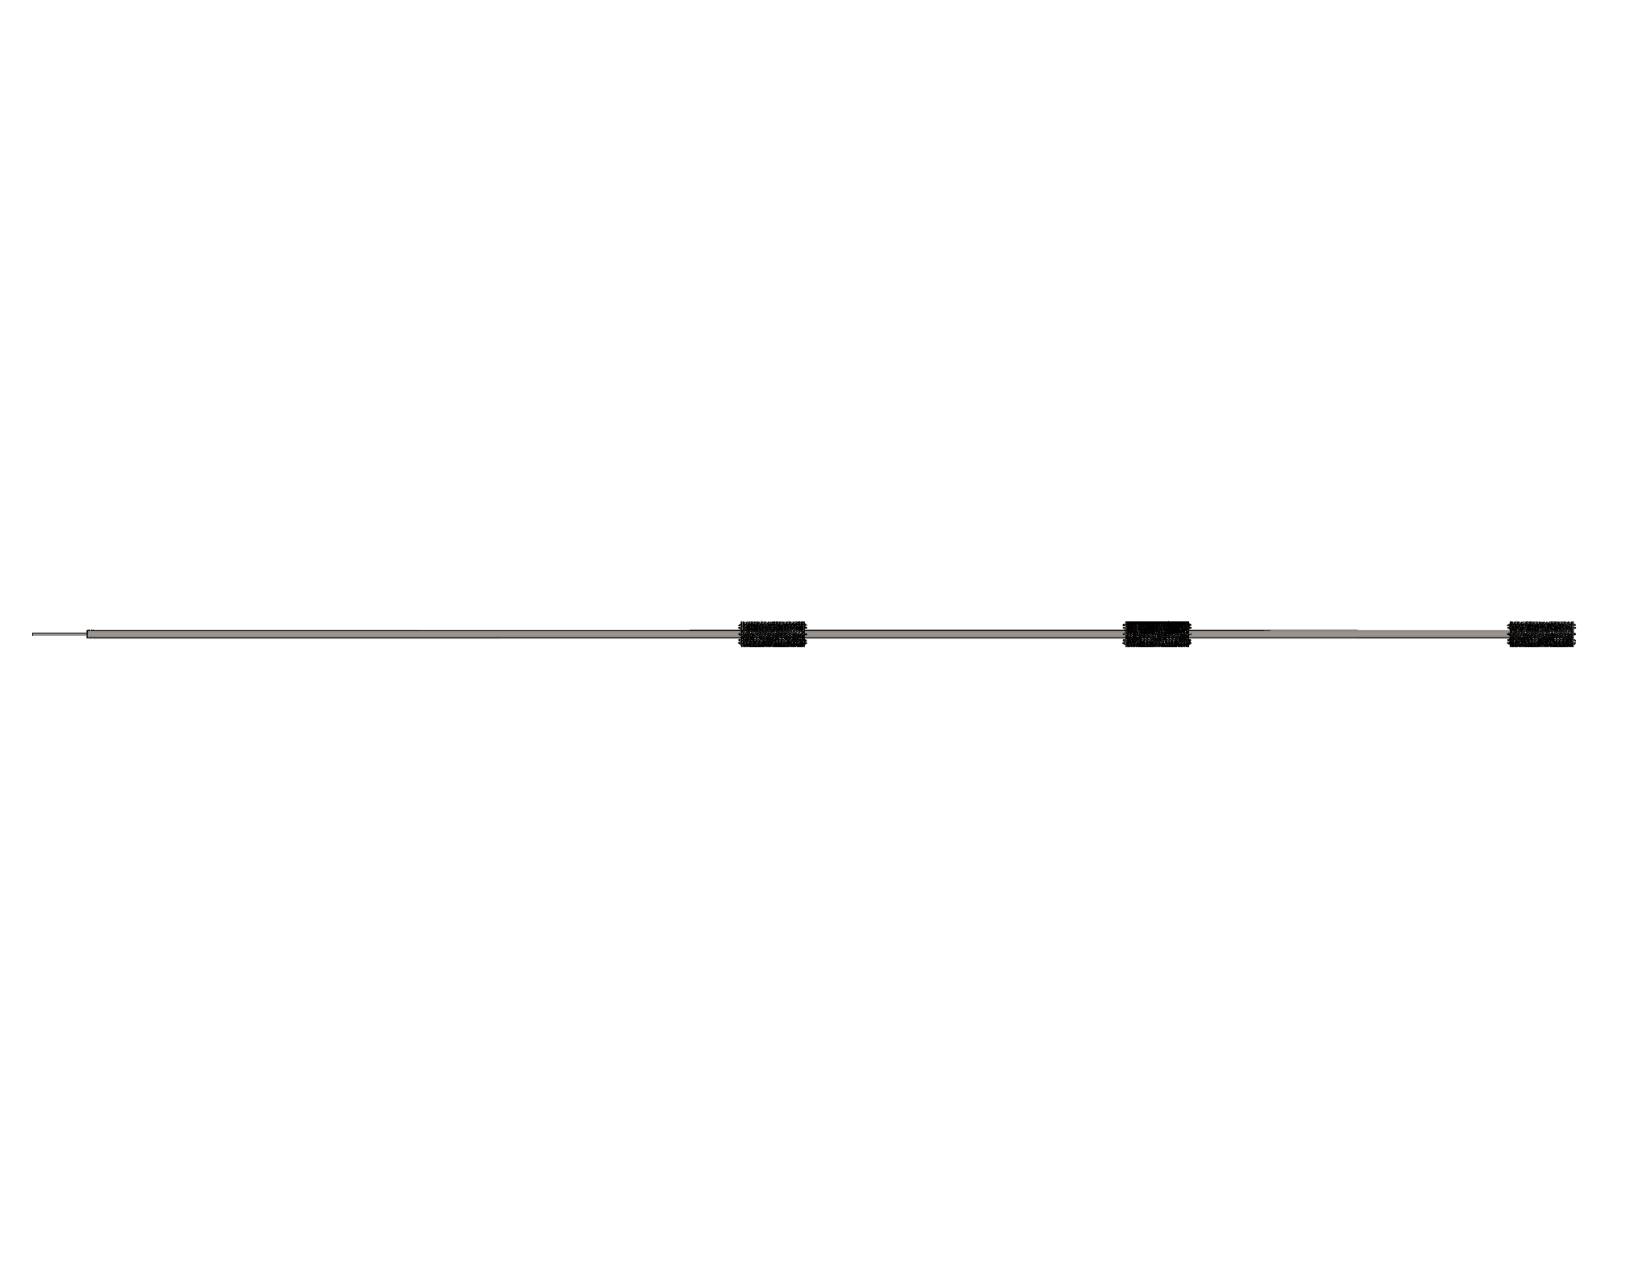
\includegraphics[width=0.9\textwidth]{PrMon-SystemString.pdf}
\end{dunefigure}



%\begin{dunefigure}[Purity Monitor String Assembly]{fig:PrMon-Assembly}
%  {Assembly sequence of the purity monitors.}
%  \includegraphics[width=\textwidth]{PrMon-Assembly.pdf}
%\end{dunefigure}



A short version of the assembly with all purity monitors will be tested in the liquid argon test facility. The full string assembly will be installed and shipped to the \dword{fd} site. A vacuum test in a long vacuum tube will be performed onsite before inserting the full assembly into the \dword{fd} cryostat. 

%not clear if we want to ship the 12 meter assembly or assemble onsite yet.
%Each monitor is assembled as the string is built from the top down, and in the end %there would be 
%three individual purity monitors %hanging 
%hang from a single string.  The assembly of the string concludes once the purity monitors are each in %place, but with the Faraday cages removed and the \dword{hv} cables and optical fibers yet to be run.  
%This full string assembly is then %would then be 
%shipped to the \dword{fd} site for installation into the cryostat. // a shorter version need to be tested in the LAr testing facility



\subsection{Thermometers}
\label{sec:fdsp-cryo-therm}
As mentioned above \fixme{Identify the section instead of saying above.} , a detailed 3D temperature map is important in monitoring whether the cryogenic system is functioning correctly and the LAr is uniform.
Given the complexity and size of purity monitors, they can only be installed on the sides of the cryostat to provide a local measurement of
LAr purity. While a direct measurement of the LAr purity across the entire cryostat is not viable, a sufficiently detailed 3D temperature map
can predict LAr purity using CFD simulations. The vertical coordinate is especially important because it will be closely related to
LAr recirculation and uniformity. 

The baseline sensor distribution and the cryostat ports used to extract cables (with indication of number of cables per port) are shown in Figure~\ref{fig:cisc-tsensor-map}. The baseline distribution will evolve as more information becomes available (precise CFD simulations, better understanding of DSS ports, installation interfaces with other groups), but the baseline suffices to establish the overall strategy.

\begin{dunefigure}[Distribution of temperature sensors inside the cryostat]{fig:cisc-tsensor-map}
  {Distribution of temperature sensors inside the cryostat}
  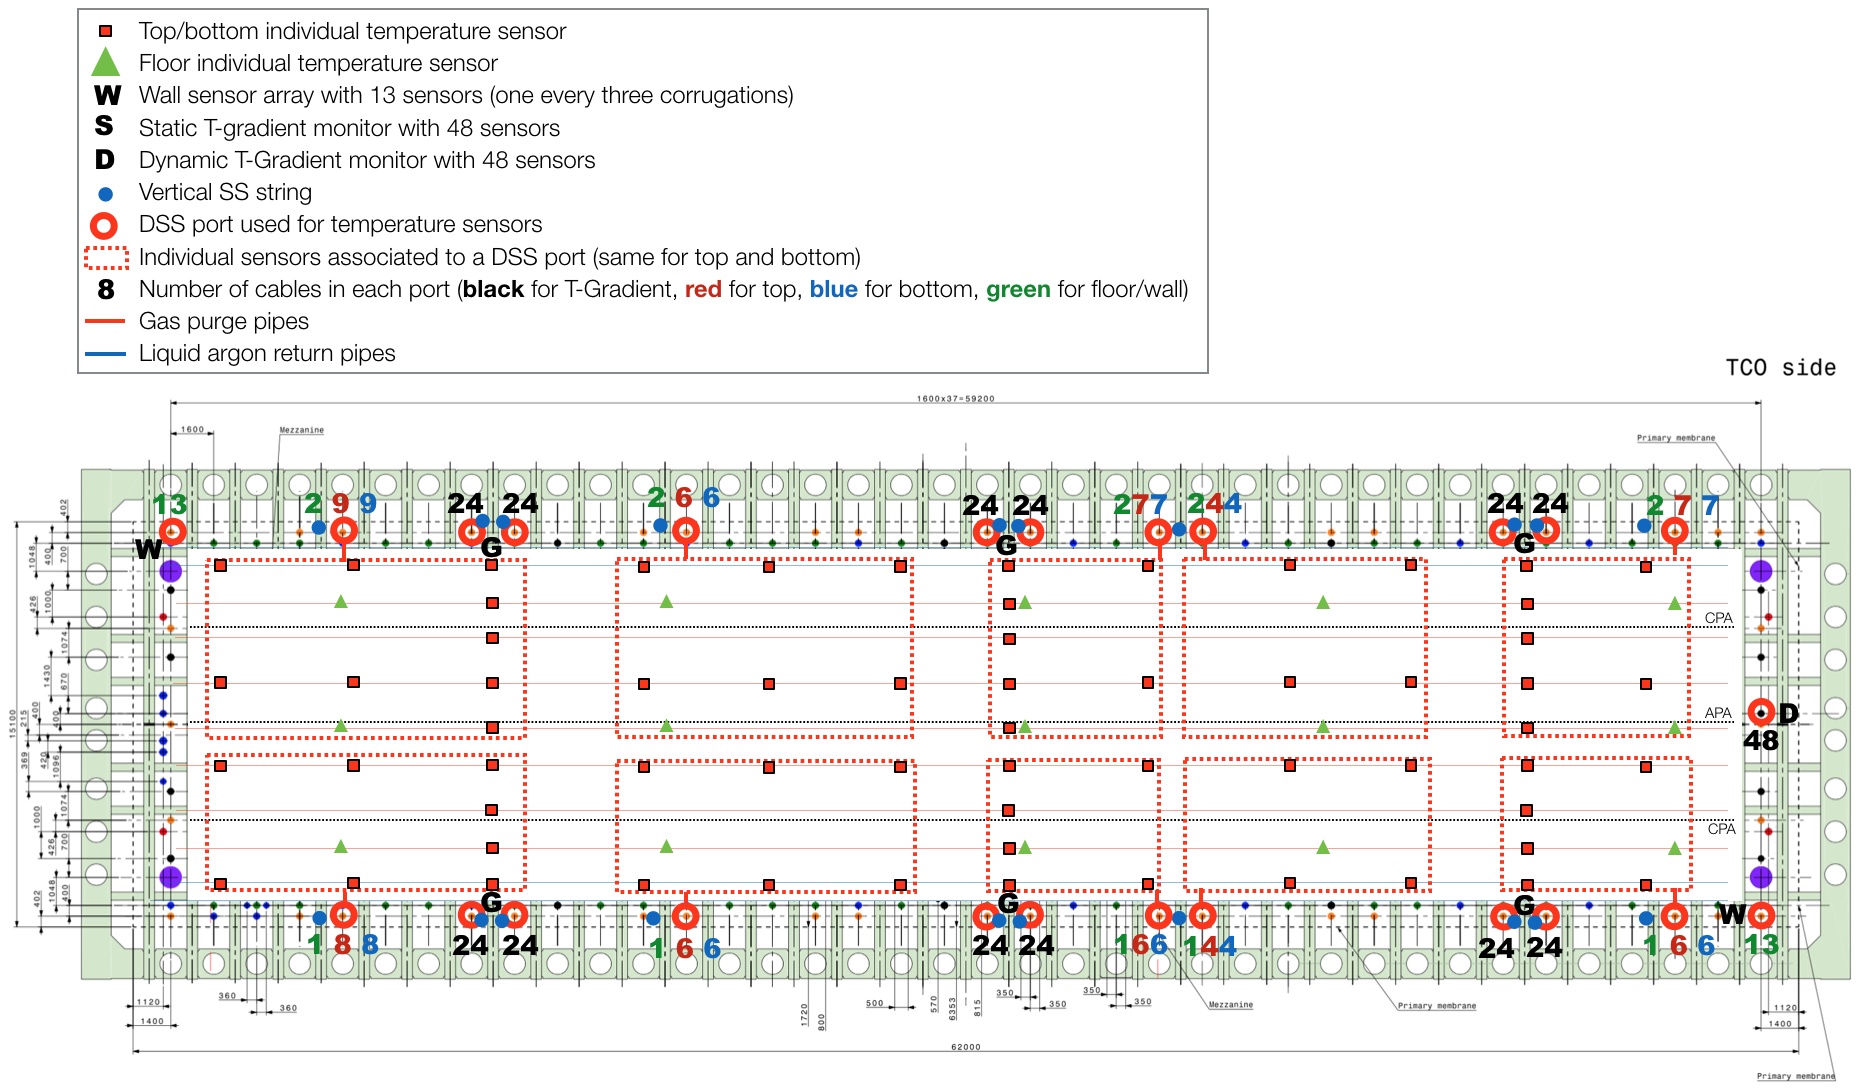
\includegraphics[width=0.9\textwidth]{cisc_tsensor_map.png}
\end{dunefigure}

High precision temperature sensors will be distributed near the TPC walls in two ways:
i) forming high density (\(>2\) sensors/\si{m}) vertical arrays (the so-called T-gradient monitors) and ii) in coarser ($\sim$ 1 sensor/\SI{5}{m}) 2D arrays (the so-called individual sensors) at the top and bottom of the detector, which are the most delicate regions. 

\fixme{I noticed in going through this section that T-gradient is occasionally presented as T-Gradient. Which is correct? That should be made consistent throughout. I assumed that the lower case is correct and changed as many as I could find. Double check that I got them all. This should include headings, which I didn't try to fix.}

Temperature variations inside the cryostat should be very small ($\SI{0.02}{K}$; see Fig.~\ref{fig:cfd-example}), %\todo{Missing figure in Thermometers intro --> \textbf{Anselmo(?) to copy figure from IDR.}}, to properly measure the 3D temperature map 
so sensors must be cross-calibrated to more than $\SI{0.005}{K}$. Most sensors will be calibrated in the laboratory before they are installed.
(Installation is described in section \fixme{Add the section number}). Where available space is restricted, the only viable way to install sensors is on the long sides of the detector
% (behind the APAs for SP, and behind the lateral FC end-walls for DP) 
and top/bottom of the detector. 
Given the precision required and the unknown longevity of the sensors, possibly requiring another  calibration after some time, a complementary method
will be used for T-gradient monitors behind the front end-walls.
% at least for the SP detector.
In areas with sufficient space for a movable system, this can be used to cross calibrate
the temperature sensors  {\em in situ}. This calibration method is described in the section about dynamic T-gradient monitors \fixme{Provide the section number for this. "...in section X on dynamic T-gradient monitors."} . 

The baseline design for all three systems, \fixme{Go ahead and relist the three systems if you think that necessary.} have three elements in common: sensors, cables, and readout system.
Platinum sensors with \SI{100}{\ohm} resistance (PT100 series), produced by Lakeshore \fixme{I think manufacturers' names have a specific format to follow.} ,  
are adequate for the temperature range, 83-92\si{K}, because, in this range, these particular sensors show high reproducibility 
$\sim\SI{5}{mK}$ and absolute temperature accuracy of \SI{100}{mK}.
Using a 4-wire readout will greatly reduce issues related to lead resistance, any parasitic resistances,
connections through the flange, and general electromagnetic noise pick-up. The Lakeshore PT102 sensors
%(see Fig.~\ref{fig:sensor_cable}-Left)
were used in the 35t prototype and ProtoDUNE-SP detector,
giving excellent results. For the inner readout cables, a custom cable made by Axon is the baseline. It consists of four teflon-jacketed 
copper wires (AWG28), forming two twisted pairs, with a metallic external shield
and an outer teflon jacket.
%Further details are given in Fig.~\ref{fig:sensor_cable}-Right. 
The readout system will be described below in a separate subsection \fixme{Again, a specific section number is needed here.} . 

%As shown in Fig.~\ref{fig:sensor_cable}, the PT102 sensor has a length of \SI{21}{mm}, which can easily be accommodated in the DUNE T-gradient monitors. 

%\begin{dunefigure}[DUNE baseline choices for sensor and cable]{fig:sensor_cable}
%  {DUNE baseline choices for sensor and cable. Left: Schematic diagram of the PT102 sensor from the Lakeshore company. Right: Schematic diagram and properties of the four wires cable from the
%  Axon company}
%  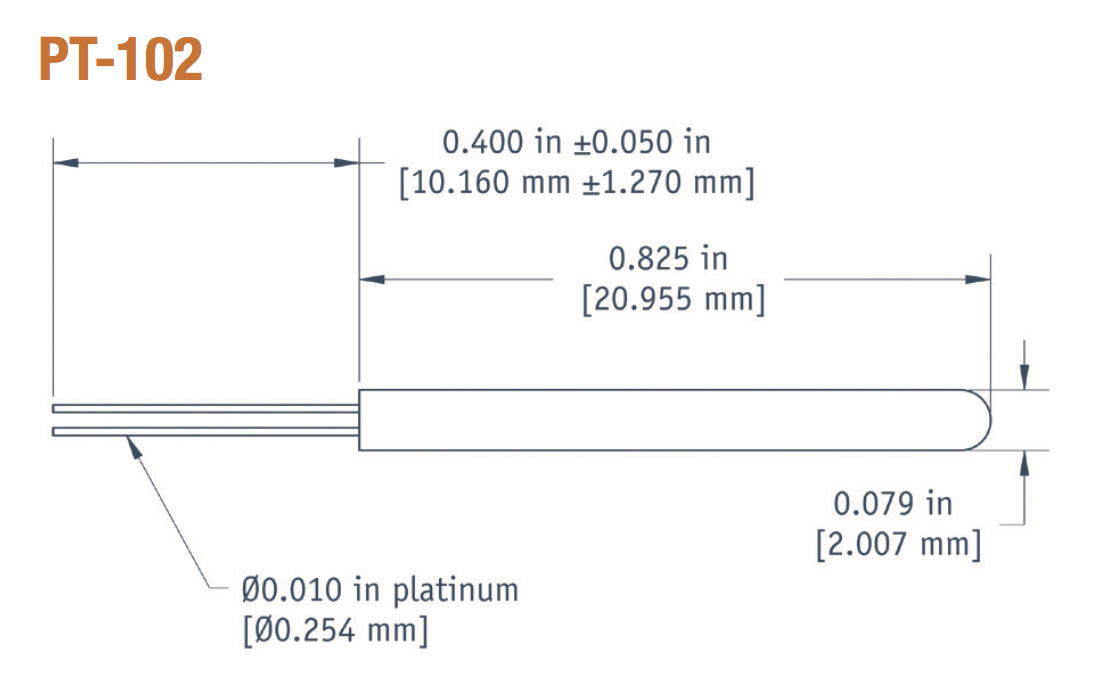
\includegraphics[width=0.4\textwidth]{cisc_pt102.png}
%  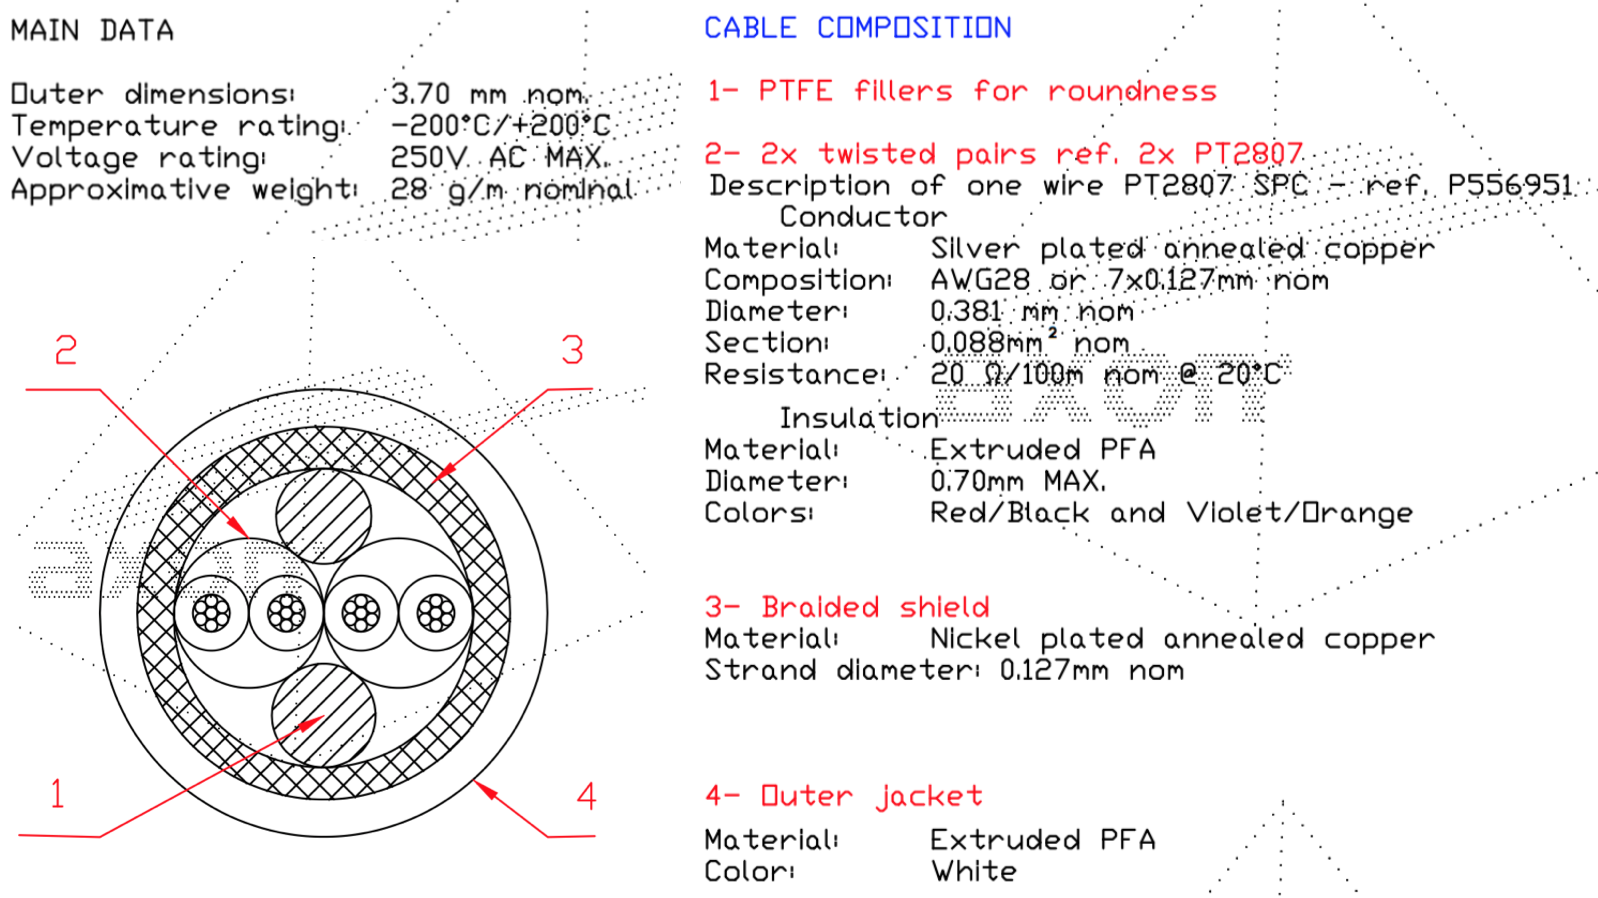
\includegraphics[width=0.55\textwidth]{cisc_TAxonCable.png}
%\end{dunefigure}

Another set of lower precision sensors epoxied into the bottom membrane of the cryostat will monitor filling the cryostat in the initial stage.   
Finally, the inner walls and roof of the cryostat will have the same types of sensors to monitor the temperature during cool-down and filling (W sensors in Figure~\ref{fig:cisc-tsensor-map}).
 
% \fixme{Remove references to DP -- done}
 
%except for the membrane sensors that may come from Minco.

% % % %
\subsubsection{Static T-Gradient monitors}

Several vertical arrays of high precision temperature sensors cross-calibrated in the laboratory will be installed behind the APAs.  
% near the lateral walls.
%(behind the APAs for SP and behind the lateral FC end-walls for DP). 
%For the SP detector, since the electric potential is zero behind the APAs, no electric field shielding is required, simplifying enormously the mechanical design.
%\footnote{This does not apply for the DP detector, for which the proper shielding must be provided.} 
The baseline design assumes six arrays with 48 sensors each. Spacing between sensors
is 20 cm at the top and bottom and 40 cm in the middle area. This configuration is similar to the one used in \dword{pdsp} but with nearly double the spacing. Figure \ref{fig:cisc-cfd-valid} shows a configuration with 48 sensors was appropriate in \dword{pdsp}, so it should also be appropriate in DUNE where the expected total gradient is no larger than in \dword{pdsp} (see Fig.~\ref{fig:cfd-example}). 

\begin{dunefigure}[Temperature sensor resolution and reproducibility]{fig:Trepro}{
 Left:   Temperature offset between two sensors as a function of time for four independent immersions in LAr. The reproducibility of those sensors, defined as the RMS of the mean offset in the flat region, is $\sim \SI{1}{mK}$,
    The resolution for individual measurements, defined as the RMS of one offset in the flat region, is more than \SI{0.5}{mK}. Right: Difference between the mean offset obtained with two independent calibration methods for the 51 calibrated sensors. The standard deviation of this distribution is interpreted as precision of the calibration.}
  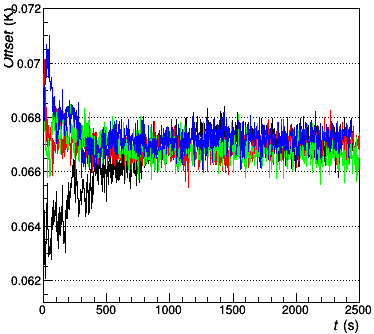
\includegraphics[height=0.44\textwidth]{cisc_tsensor_calib.png}%
  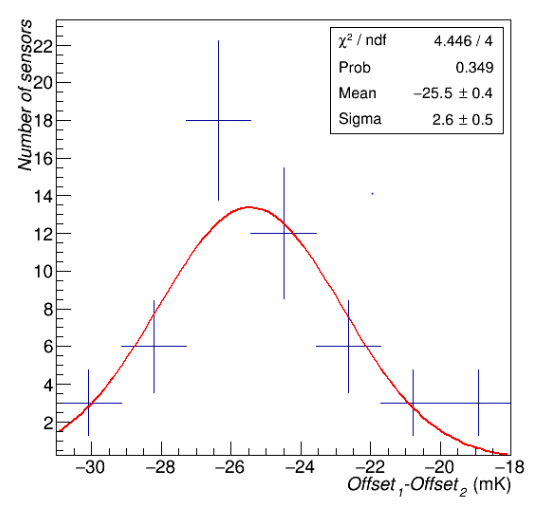
\includegraphics[height=0.45\textwidth]{cisc_tsensor_calib2.png}%
\end{dunefigure}

Sensors are cross-calibrated in the laboratory using a controlled environment and a high precision readout system, described below in a separate subsection \fixme{The section should be named.} .
%Although the calibration procedure will certainly improve, the one currently used for ProtoDUNE-SP is descrived here.
%Four sensors are placed as close as possible (such that identical temperature can be assumed for all of them) inside a small cylindrical aluminum capsule,
%which protects the sensors from thermal shocks and helps in minimizing convection.
%One of the sensors acts as reference while the other three are the ones being calibrated. Five independent calibrations
%are performed for each set of three sensors, such that the reproducibility of each sensor can be computed. For each calibration 
%the capsule is introduced in a PLA box of size \(9.5\times9.5\times\SI{19}{cm^3}\), with two concentrical independent volumes of LAr
%and sourounded by a polystyrene box with \SI{15}{cm} thick walls. A small quantity of LAr is used to slowly
%cooldown the capsule to $\sim\SI{90}{K}$, avoiding thermal shocks that could dammage the sensors.
%Then the capsule is covered by LAr such that it penetrates
%inside fully covering the sensors. Once the temperature stabilizes to the 1-\SI{2}{mK} level (after 5-15 minutes) measurements are taken. Then the capsule is taken out from LAr
%and kept at room temperature until it reaches \SI{200}{K}. As mentioned above, this procedure is repeated five times, before going to the next set of three sensors.  
As Figure ~\ref{fig:Trepro} shows, the calibration of ProtoDUNE-SP sensors was precise to $\SI{2.6}{mK}$. This was confirmed using ProtoDUNE-SP temperature data (see Figure~\ref{fig:cisc-cfd-valid}), where the difference in temperature measured by two adjacent sensors is consistent with precision of $\SI{2.6}{mK}$.  


\begin{dunefigure}[Conceptual design of the Static T-Gradient monitor]
{fig:cisc-static-tgradient}
  {Conceptual design of the Static T-Gradient monitor.}
  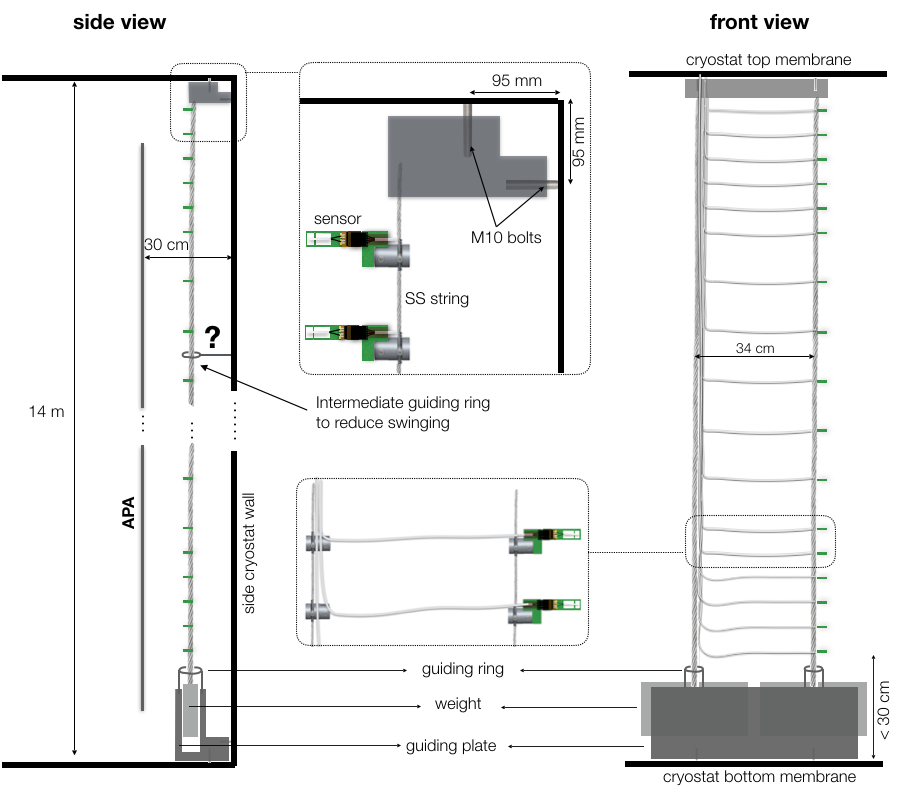
\includegraphics[width=0.8\textwidth]{cisc_static_tgradient.png}
\end{dunefigure}
\fixme{Is "Static T-Gradient" a proper noun (and thus capitalized)? Other figures do not use capitals in the titles other than for the first word.}

Figure~\ref{fig:cisc-static-tgradient} shows the baseline design for the mechanics 
%of the SP system . It consists in two stainless steel strings anchored at top and bottom corners of the cryostat
\fixme{Mechanics of what?}
using the available M10 bolts (see Fig.~\ref{fig:sensor-support}-Left). One string routes the cables while the other,
separated \SI{340}{mm}, \fixme{I read this as "One string routes the cables while the other, separated from the first by \SI{340}{mm} supports the temperature sensors."} supports the temperature sensors.
Given the height of the cryostat, an intermediate anchoring point is needed to reduce swinging. That is still under discussion. To account for shrinkage in the strings under cryogenic conditions and to guarantee that the same tension is always applied, a weight is hung at the bottom of the strings. A guiding system made of stainless steel and anchored at four M10 bolts at the bottom keeps the weight confined in space. A prototype is being built at IFIC, where the full system will be mounted using two dummy cryostat corners. We are also considering an alternative design with carbon fiber strings.  

% \fixme{Static T-Gradient: comment out reference to dual phase? [gahs] --- I took the liberty of doing this myself [gahs]}
% For the DP detector no baseline design exists yet,
% since additional complications due to the required electric field shielding must be taken into account. 
% \todo{Is the second sentence in this paragraph about dual phase? Why does paragraph begin with dual phase? [gahs]}

Fig.~\ref{fig:sensor-support}-Right shows the baseline design of the
PCB support for temperature sensors with an IDC-4 male connector. 
It is $52\times \SI{15}{mm^2}$. A narrower connector (with two rows of two pins each) is being studied. This alternative design would reduce the width of the PCB assembly and allow more sensors to be calibrated simultaneously. Each four-wire cable from the sensor to the flange will have an IDC-4 female connector on the sensor side; on the other side \fixme{We have the sensor side; what is the "other" side?} , it will be soldered/crimped to the appropriate connector, whose type and number of pins (SUBD-25 connectors were used in ProtoDUNE-SP) depend on the final design of the DSS ports that will be used to extract the cables. 

\begin{dunefigure}[Cryostat bolts and temperature sensor support]{fig:sensor-support}
  {Left: bolts at the bottom corner of the cryostat. Right: Lakeshore PT102 sensor mounted on a PCB with an IDC-4 connector.}
  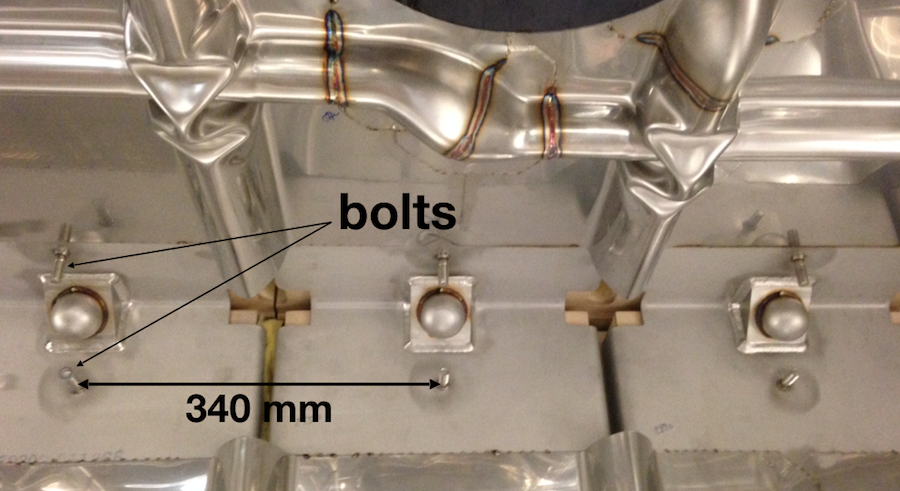
\includegraphics[height=0.2\textwidth]{cisc_cryostat_bolts.png}%
    \hspace{1cm}%
  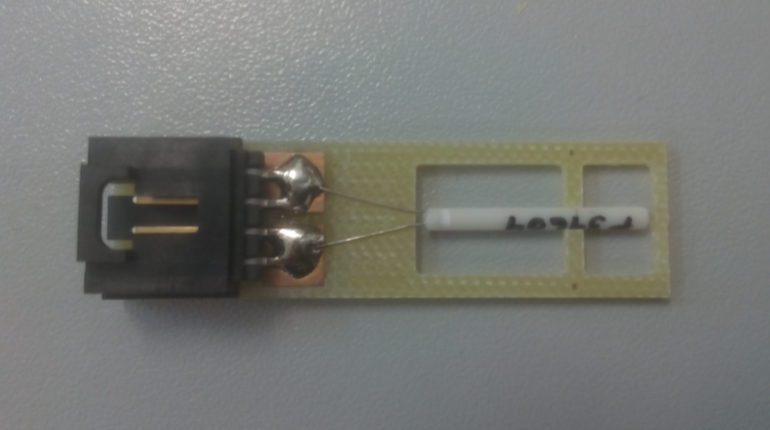
\includegraphics[height=0.2\textwidth]{cisc_tsensor.png}%
\end{dunefigure}




% \begin{dunetable}
% [Static t-gradient parameters]
% {p{0.2\textwidth}p{0.1\textwidth}p{0.6\textwidth}}
% {tab:fdgen-cisc-static-tgradient}
% {Parameters for the Static T-gradient monitor}   
% Parameter            & {\bf value} & {\bf comment} \\ \toprowrule
% \# sensors	         &     48      &       \\ \toprowrule
% sensor spacing       &    20/40 cm & 20 at top and bottom and 40 in the mid area  \\ \toprowrule
% cable diameter       &   3.5 mm    &       \\ \toprowrule
% cable weight         &   28 g/m    &       \\ \toprowrule
% cable-string weight  &   13 Kg     &  10 Kg for the cable, 1.3 Kg for the SS string and 1.7 kg for the cable supports      \\ \toprowrule
% sensor-string weight &   3.3 Kg     & 1.3 Kg for the SS string, 1.7 kg for the cable supports and 300 g for the sensors     \\ \toprowrule
% \end{dunetable}

%Table \ref{tab:fdgen-cisc-static-tgradient} summarizes key properties of the static T-gradient monitor.

% % % %
\subsubsection{Dynamic T-Gradient monitors}

% What I was thinking about is to have 3 sensors per meter. 4 would be even better and have 1.35 m range of motion. The goal is to have 4 sensor overlap. In this case, we would be quite safe against sensor failure.
% If we are to populate 14 m with 3 sensors per meter, that would be 42 sensors. In addition, we should increase frequency at the top or bottom.

The dynamic temperature monitor is a vertical array of high precision temperature sensors to measure the vertical temperature gradient within a few mK. The design of the system is driven by the following:
\begin{itemize}
\item
Few mK uncertainties in the measured vertical temperature profile over the entire detector height are required to monitor LAr purity and provide useful feedback on the efficiency of cryogenic recirculation and purification.
\item
Simulations of cryogenic recirculation predict very slow changes in temperature at meter scale except at the bottom and top of the cryostat. Thus, sensors will be placed every \SI{50}{cm} along the detector height with more sensors in the first \SI{50}{cm}, closest to the bottom of the cryostat, and the last \SI{50}{cm}, closest to the top of the cryostat, where spacing between sensors is reduced to \SI{10}{cm}.
 \end{itemize}


To address concerns about potential differences in sensor readings before and after installation in DUNE FD, the dynamic temperature monitor \fixme{Please check this phrasing. I could not determine exactly where that comma should go, and it is an important comma.} allows cross-calibration of sensors in situ \fixme{In situ should be in italics.} . Namely, this T-gradient monitor  can move vertically while installed in DUNE FD, which allows precise cross-calibration between sensors in situ \fixme{Again, in situ should be in italics.} at predefined locations as well as between them \fixme{Here, the word "them" may refer to locations or to sensors. This must be clear.} . \fixme{This entire procedure is unclear. Shorten the sentences and make the procedure description more precise. A figure might help, along with references to that figure in the text.} The procedure for cross-calibration involves first, taking a temperature reading at the lowest sensor position. Then, the stepper motor moves the carrier rod up by \SI{50}{cm} putting all sensors in the location of their neighbor that is \SI{50}{cm} above them. Then the second reading is taken. In this manner, except for the lowest position we have temperature measurement at each location with two adjacent sensors, and by linking the temperature offsets between the two readings at each location, temperature readings from all sensors are cross-calibrated in situ \fixme{Remember to put this in italics.} , canceling all offsets due to electromagnetic noise or any parasitic resistances that may have prevailed despite the four point connection to the sensors that should cancel most of the offsets. These measurements are taken with very stable current source, which ensures high precision of repeated temperature measurements over time. The motion of the dynamic T-monitor is stepper motor operated, delivering measurements with high spatial resolution. 

This procedure was tested in ProtoDUNE-SP, where the system was successfully moved up by a maximum of 51 cm, allowing cross-calibration of all sensors (22 sensors with 10.2 cm spacing at top and bottom and 51 cm in the middle). 
Figure~\ref{fig:cisc-cfd-valid} shows the temperature profile after calibration; the smoothness of the profile demonstrates the reliability of the method.  

\todo{Figure on the dynamic profiler movement  to be inserted when available. }

\subsubsection{Dynamic T-gradient monitor design}
A dynamic T-gradient monitor has three parts: a carrier rod on which sensors are mounted; an enclosure above the cryostat housing space that allows the carrier rod to move vertically   1.5\,m over its lowest location; and the motion mechanism. The motion mechanism consists of a stepper motor connected through a ferrofluidic dynamic seal to a gear and pinion motion mechanism. The sensors have two pins soldered to a printed circuit board (PCB). Two wires are individually soldered to the common soldering pad for each pin.  A cutout in the PCB around the sensor allows free flow of argon for more accurate temperature readings.  Stepper motors typically have very fine steps that allow highly precise positioning of the sensors.  Figure~\ref{fig:fd-slow-cryo-dt-monitor-overview} shows the overall design of the dynamic T-gradient monitor with the sensor carrier rod, enclosure above the cryostat, and stepper motor mounted on the side of the enclosure. The enclosure has two parts connected by a 6-cross flange. One side of the 6-cross flange will be used for signal wires, another will be used as a viewing window, and the two other ports will be spares. Figure~\ref{fig:fd-slow-cryo-sensor-mount}-Left shows the PCB mounted on the carrier rod and the sensor mounted on the PCB along with the four point connection to the signal readout wires. Finally, Figure~\ref{fig:fd-slow-cryo-sensor-mount}-Right shows the stepper motor mounted on the side of the rod enclosure. The motor remains outside the enclosure, at room temperature, and its power and control cables also remain outside.

\begin{dunefigure}[Dynamic T-gradient monitor overview]{fig:fd-slow-cryo-dt-monitor-overview}
  {An overview of the dynamic T-gradient monitor.}
% 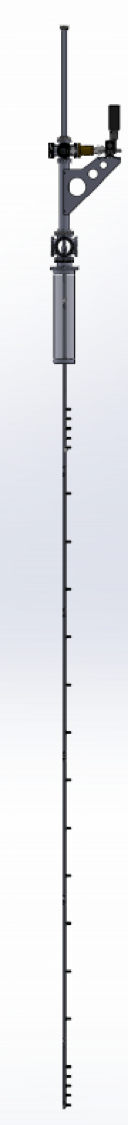
\includegraphics[width=0.11\textwidth,angle=90]{cisc_DTOverview.png}
 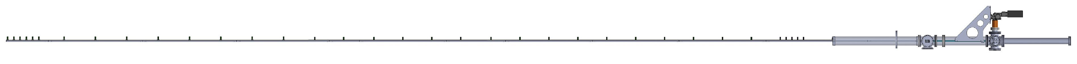
\includegraphics[width=0.95\textwidth,angle=0]{cisc_DynamicProfiler.png}
\end{dunefigure}
\begin{dunefigure}[Sensor-cable assembly for dynamic T-gradient monitor]{fig:fd-slow-cryo-sensor-mount}
  {Left: Sensor mounted on a PCB board and PCB board mounted on the rod. Right:
    The driving mechanism of the dynamic T-gradient monitor, consisting of a stepper motor driving the pinion and gear linear motion mechanism. }
  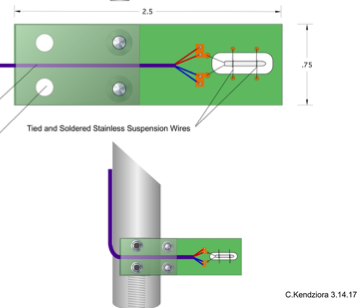
\includegraphics[width=0.40\textwidth]{cisc_DTSensorMount.png}
  \hspace{3cm}%
  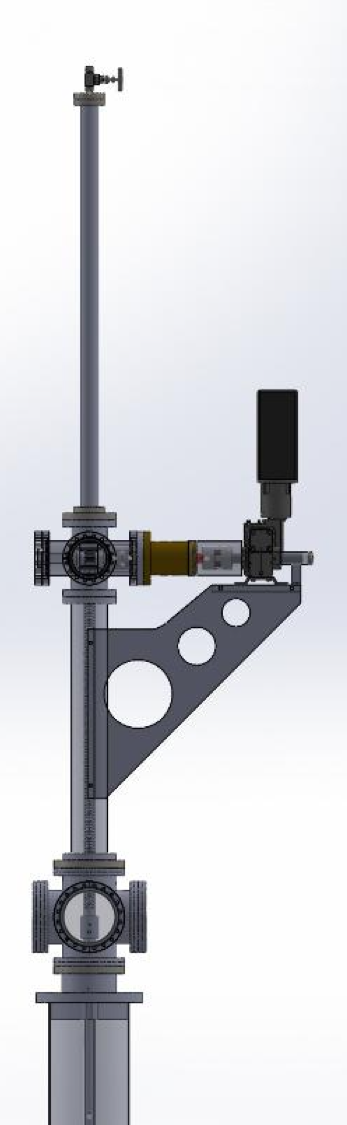
\includegraphics[width=0.12\textwidth]{cisc_DTMotor.png}
\end{dunefigure}

% % % %
\subsubsection{Individual Temperature Sensors}

T-gradient monitors will be complemented by a coarser 2D array (every 5 m) of precision sensors at the top and bottom of the detector, as shown in Figure~\ref{fig:cisc-tsensor-map}. Following the ProtoDUNE-SP design, bottom sensors will use the cryogenic pipes as support structure, while top sensors will be anchored to the ground planes. Although sensors at the top will have a similar distribution to those at the bottom, some differences will occur because suitable anchoring points at the top and bottom will differ. 

As in ProtoDUNE-SP, another set of standard sensors will be evenly distributed and epoxied to the bottom membrane. They will detect the presence of LAr when cryostat filling starts. Finally, two vertical arrays of standard sensors will be epoxied to the lateral walls in two opposite vertical corners, with a spacing of 102 cm (every 3 corrugations), to monitor the cryostat membrane temperature during the cool-down and filling processes. 

While in ProtoDUNE-SP, cables were routed individually (without touching neighboring cables or any metallic elements) to prevent grounding loops in case the outer Teflon jacket broke, such a failure is very unlikely. Thus, in DUNE far detectors, cables will be routed in bundles, simplifying the design enormously. As Figure~\ref{fig:cisc-tsensor-map} shows, up to 20 sensors will use the same DSS port, a cable bundle 16 mm in diameter.

Cable bundles of several sizes will be configured using custom made Teflon 
pieces,  %(see Fig.~\ref{fig:cable-support})
which will be anchored to different cryostat and detector elements to route cables from sensors to DSS ports. For sensors at the bottom (on pipes and floor), cables will be routed towards the cryostat bottom horizontal corner using stainless steel split clamps anchored to pipes (successfully prototyped at \dword{pdsp}), and from there, to the top of the cryostat using vertical strings (as with static T-gradient monitors). For sensors on the top ground planes, cables bundles will be routed to the corresponding DSS port using Teflon supports attached to both the FR4 threaded rods in the union between two ground plane modules and to the DSS I-bins (both successfully prototyped at \dword{pdsp}). Sensors on the walls will use bolts in the vertical corners for cable routing. 

For all individual sensors, PCB sensor support, cables, and connection to the flanges will be the same as for the T-gradient monitors. 
  

%\begin{dunefigure}[Cable supports for individual temperature sensors]{fig:cable-support}
%  {Left: support for two cables on ground planes. Right: Supports for three %cables  mounted on cryogenics pipes using split clamps}
% This PDF is made from the .dot of the same name.
%  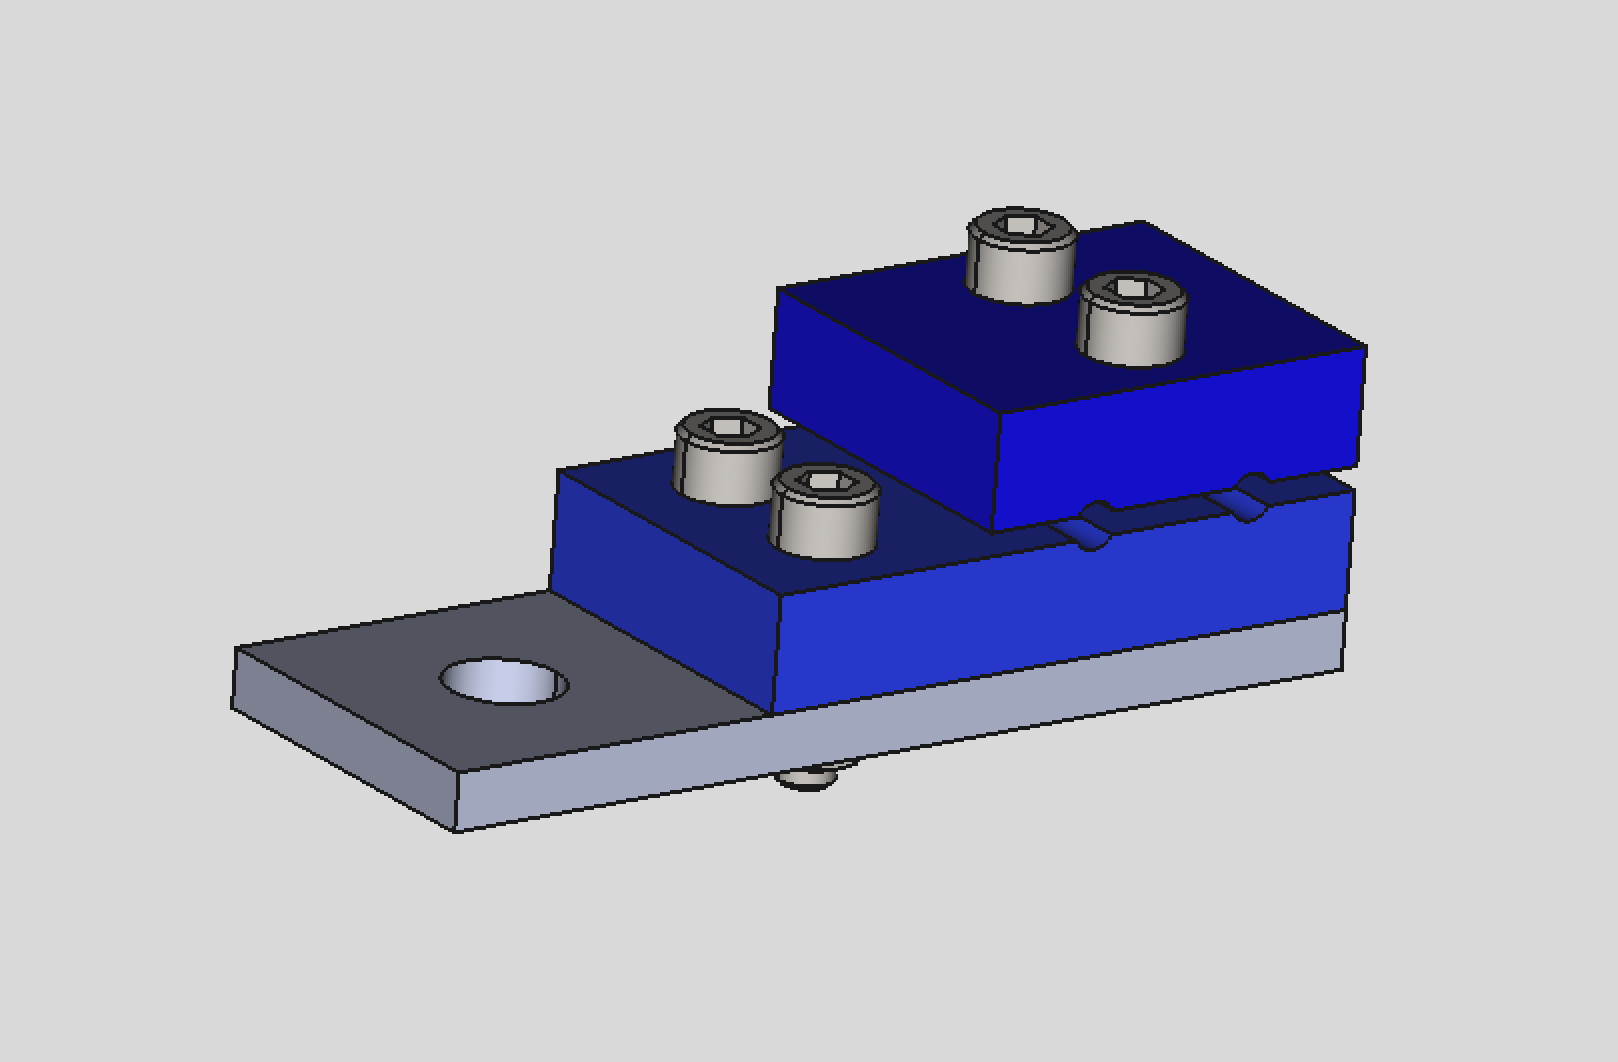
\includegraphics[width=0.3\textwidth]{cisc_TcableSupportGP.png}
%  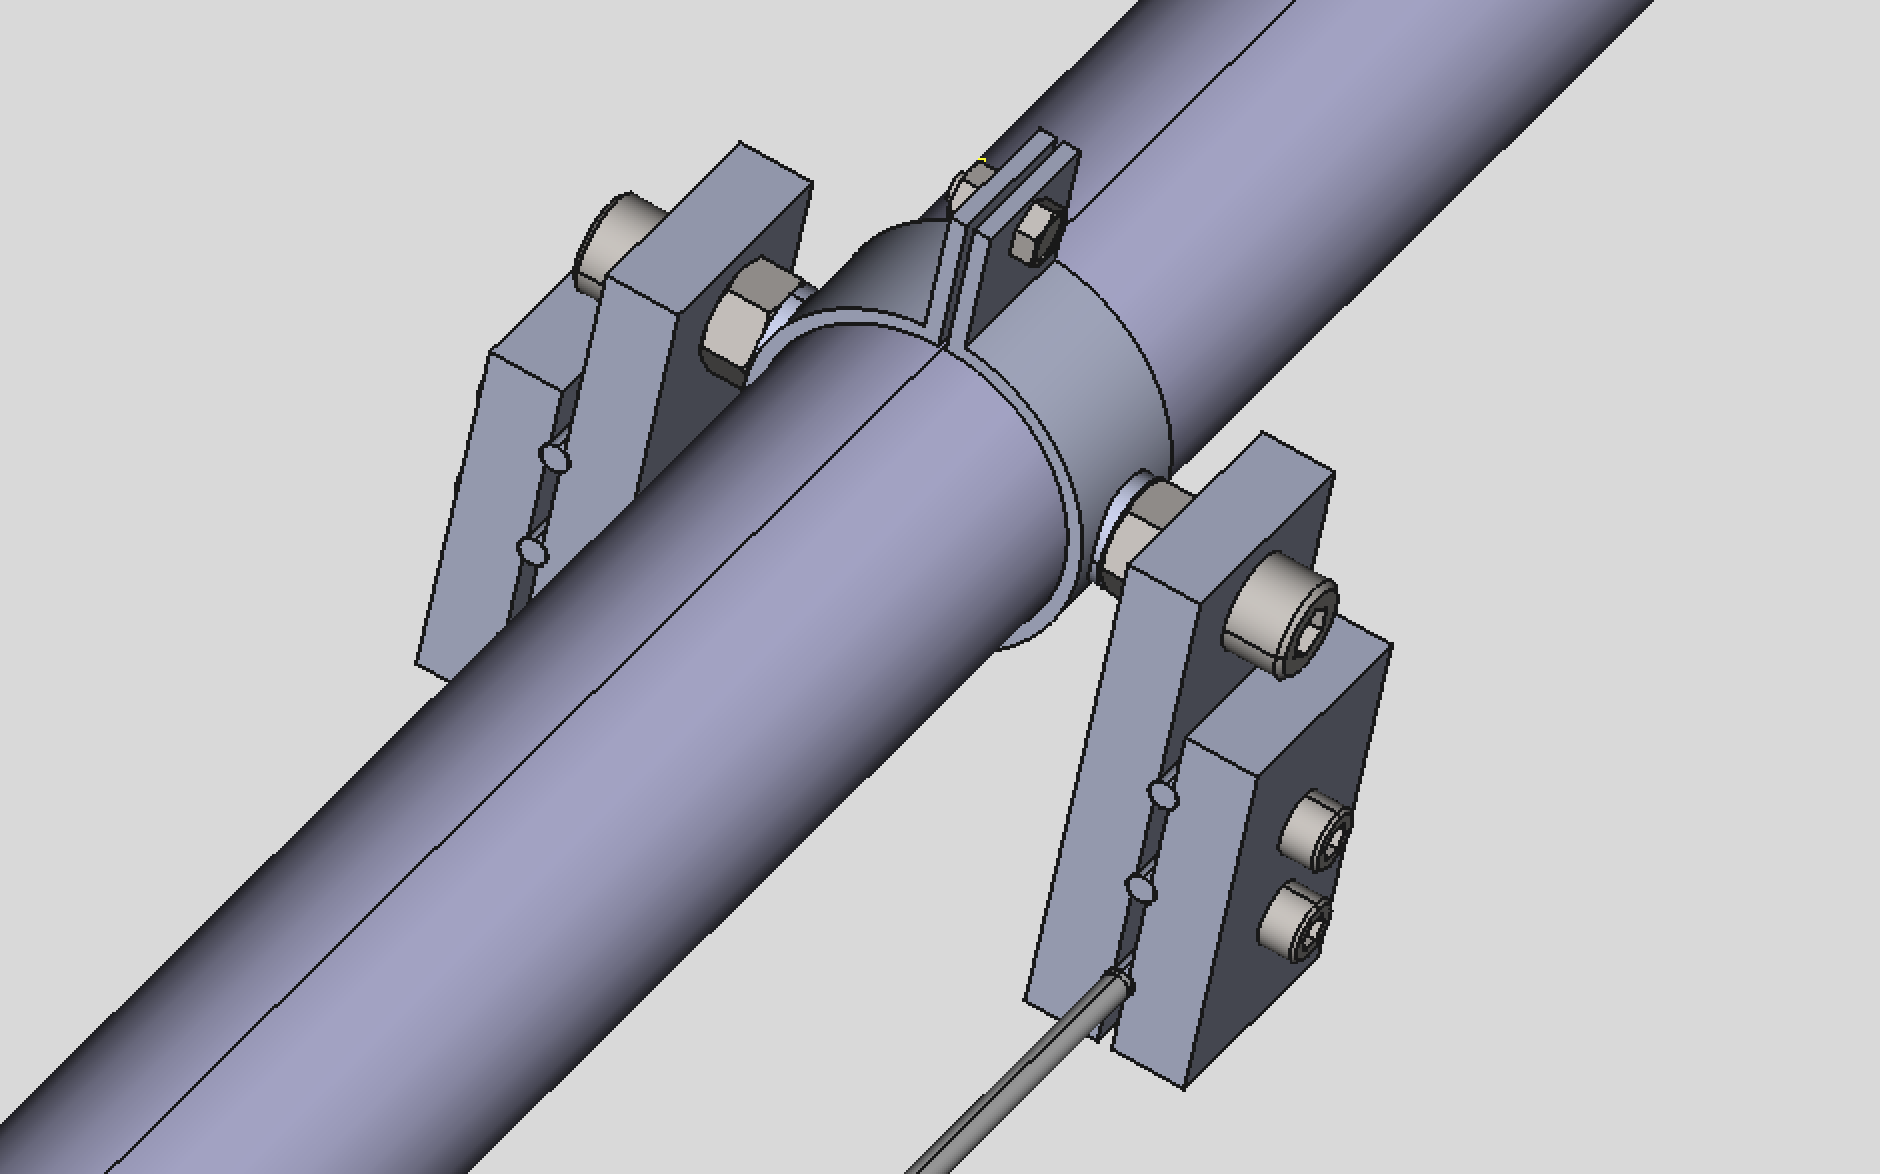
\includegraphics[width=0.315\textwidth]{cisc_TcableSupportPipes.png}
%\end{dunefigure}


% % % %
\subsubsection{Readout system for thermometers}
\label{sec:fdgen-slow-cryo-therm-readout}

A highly precise and very stable system is required to achieve a readout level of $< \SI{5}{mK}$.
The proposed readout system was used in ProtoDUNE-SP and relies on a variant of an existing mass PT100 temperature readout system developed at
CERN for an LHC experiment; it has already been tested and validated by the collaboration experts. The system has an electronic circuit that includes
\begin{itemize}
\item A precise and accurate current source for the excitation of the temperature sensors measured using the 4-wires method. 
\item A multiplexing circuit connecting the temperature sensor signals and forwarding the selected signal to a single line.
\item A readout system based on National Instrument Compact RIO Device  with a high accuracy voltage signal readout NI9238 module with 24 bit resolution over a \SI{1}{V} range. This device also drives the multiplexing circuit and calculates temperature values. The Compact RIO device is connected to the detector ethernet network, sending temperature values to the DCS software through a standard OPC UA driver.

\end{itemize}

The current mode of operation averages more than 2000 samples taken every second for each sensor. 
Figure ~\ref{fig:Trepro} shows the system has a resolution higher than \
\SI{1}{mK}, the RMS of one of the offsets in the stable region.


%%%%%%%%%%%%%%%%%%%% LIQUID LEVEL MONITORING %%%%%%%%%%%%%%%%%%%%
\subsection{Liquid Level Monitoring}
% john L, anselmo
% SP

The goals for the \lar level monitoring system are basic level sensing when filling and precise level sensing during static operations. 

Filling the cryostat with \lar will take several months. During this operation, 
the differential pressure between the top of
the cryostat and known points below can be converted to depth using
the known density of \lar.  The temperatures of \dwords{rtd} at known
heights can also be used to determine when the cold liquid reaches 
each \dword{rtd}. Fine tuning of the final LAr level will be done using 
several capacitive level meters at the top of the cryostat. 

During operation, liquid level monitoring has two purposes:
the cryogenics system uses monitoring to tune the \lar flow, and 
the detector uses monitoring to guarantee that the top \dwords{gp} are always
submerged (otherwise, the risk of dielectric breakdown is high). The plan is to keep the \lar surface at least \SI{20}{cm} above the \dwords{gp}. This was the value used for the \dword{hv} interlock in \dword{pdsp}. 

The \lar flow 
is tuned using two differential pressure level meters, installed as part of the cryogenics system, one on each side of the \dword{detmodule}.  They 
have a precision of \SI{0.1}{\%}, which corresponds to \SI{14}{mm} at the
nominal \lar surface. Cryogenic pressure sensors will be purchased from commercial sources. Installation methods and positions will be determined as part of the
cryogenics internal piping plan.  
%Sufficient redundancy will be designed in
%to ensure that no single point of failure compromises the level measurement.

%This precision is sufficient for the  \dword{spmod}, since the plan is to keep the \lar surface at least \SI{20}{cm} above the \dwords{gp} (this is the value used for the \dword{hv}
%interlock in \dword{pdsp}); thus, no additional level meters are required for the \single. 

For HV integrity, multiple capacitive level sensors (with a precision of few \fixme{This may need to be more precise.} mm) will be deployed along the top of the fluid, used during stable operation, and checked against each other.
One capacitive level sensor at each of the four corners of the cryostat will provide sufficient redundancy to ensure that no single point of failure compromises the capacitive level sensor measurement.


% However, in the \dual \lar system the surface level should be controlled at the millimeter level, which can be accomplished with capacitive monitors. Using the same capacitive monitor system in each \dword{detmodule} reduces design differences and provides a redundant system for the \single.  Either system could be used for the \dword{hv} interlock.





Figure~\ref{fig:cisc_pdsp_level} shows the evolution of the \dword{pdsp} LAr level over two months as measured by the differential pressure and capacitive level meters. 
%\fixme{Liquid Level Monitoring has ProtoDUNE results --> \textbf{Anselmo to get data, add something about this. WORK IN PROGRESS}}


\begin{dunefigure}[LAr level measurements]{fig:cisc_pdsp_level}{Evolution of the \dword{pdsp} LAr level over two months. Left: Measured by the capacitive level meter. Right: Measured by the differential pressure level meter. The units in the vertical axis are percentages of the cryostat height (7878 mm).}
  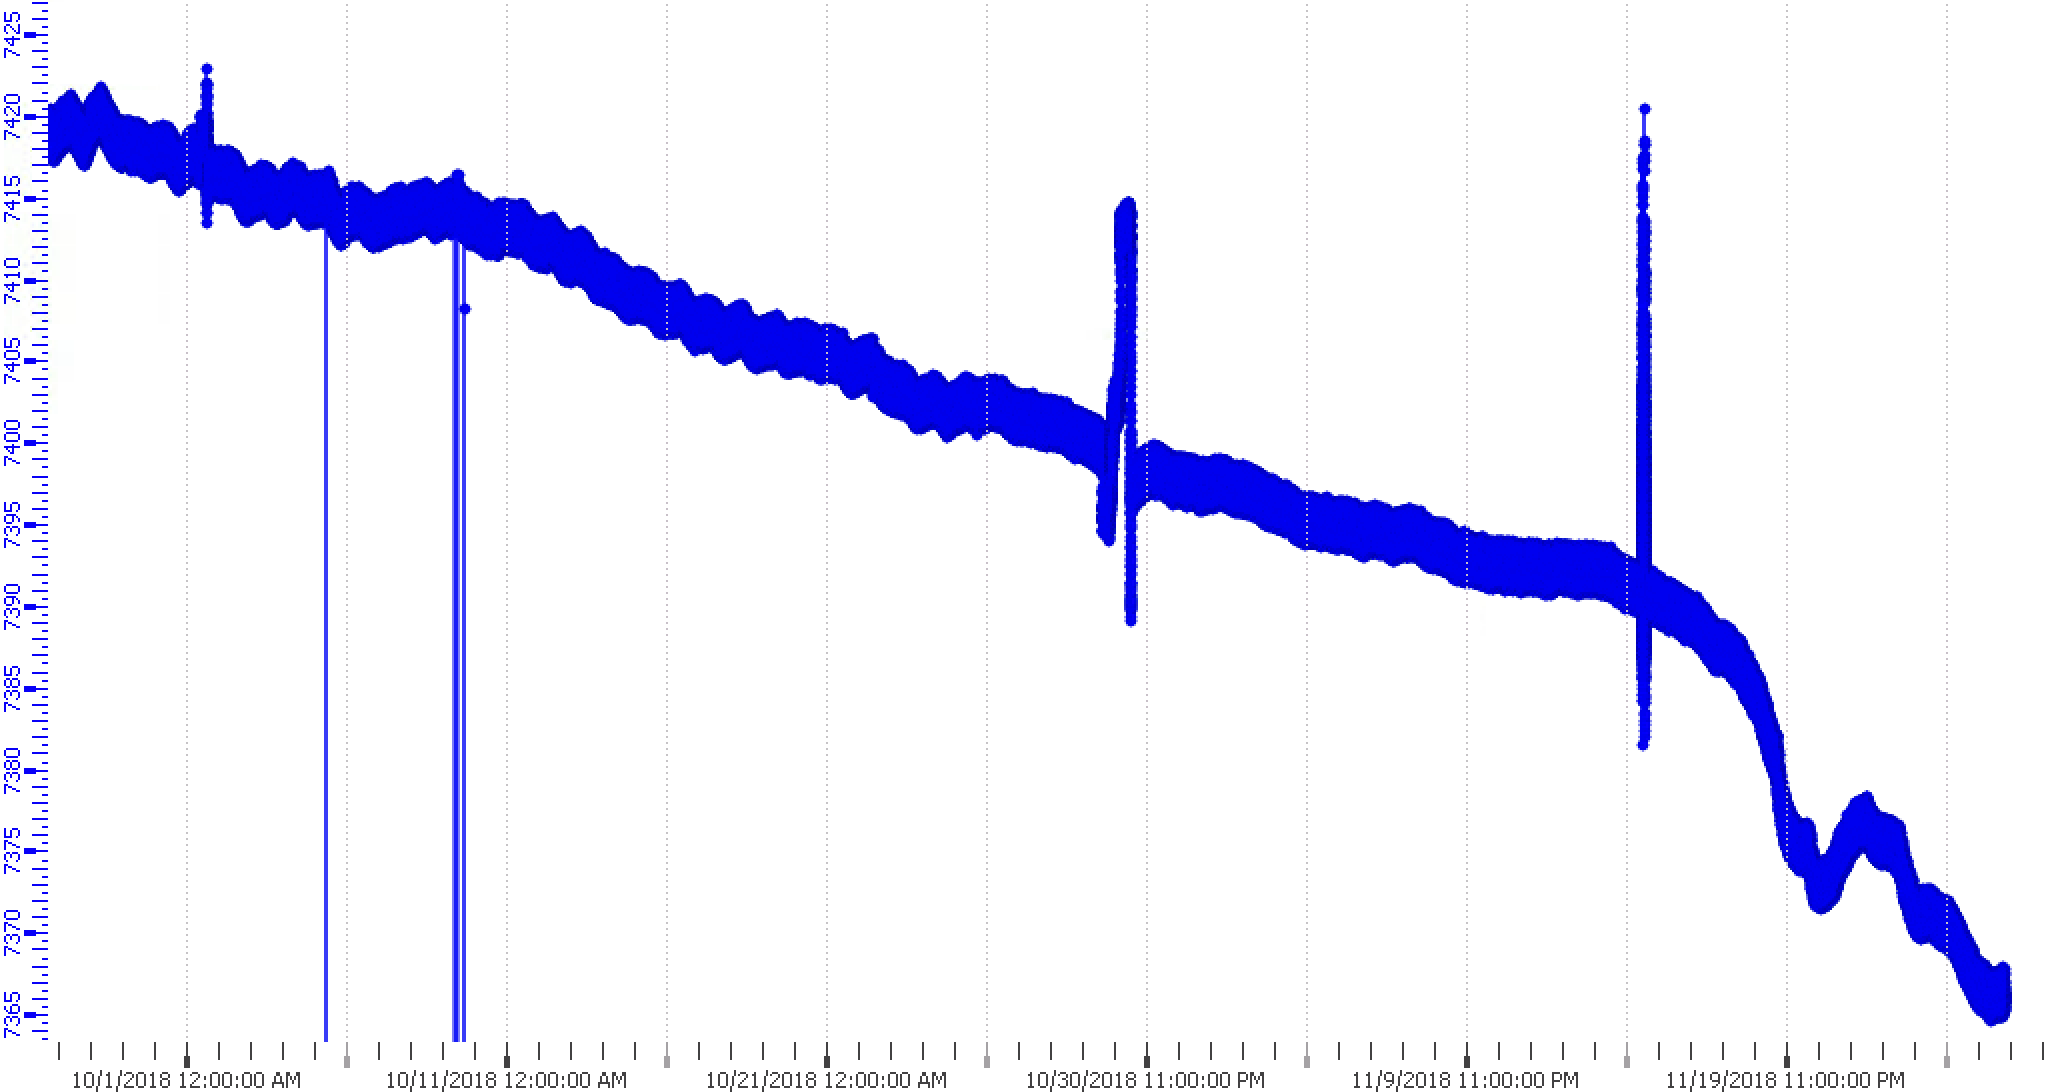
\includegraphics[width=0.4\textwidth]{cisc_level_cap.png}%
  \hspace*{1cm}
  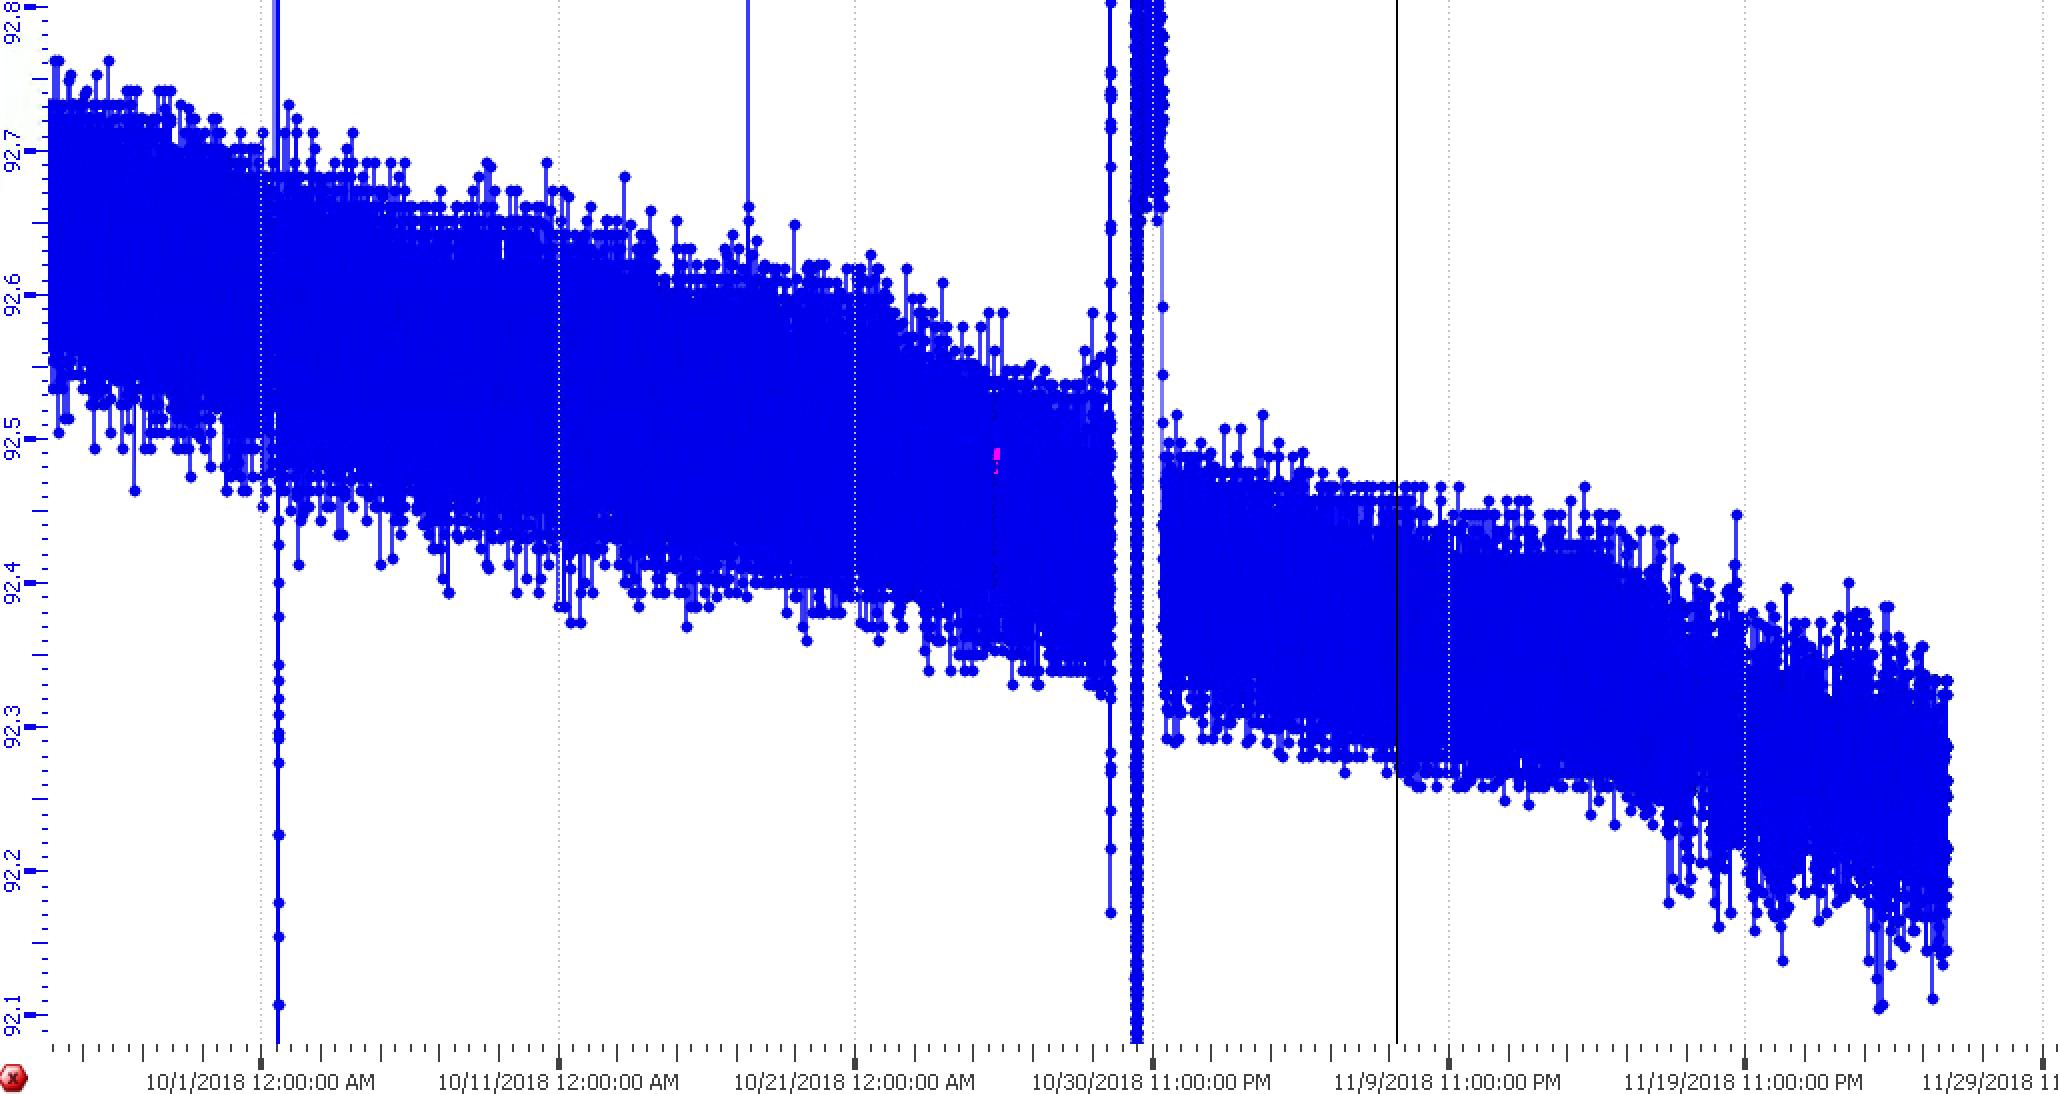
\includegraphics[width=0.4\textwidth]{cisc_level_diffp.png}%
\end{dunefigure}

%%%%%%%%%%%%%%%%%%% GAS ANALYZERS %%%%%%%%%%%%%%%%%%%%
\subsection{Gas Analyzers}
\label{sec:fdgen-slow-cryo-gas-anlyz}
% alan h

 Gas analyzers are commercially produced modules that measure trace quantities of specific gases contained within a stream of carrier gas. The carrier gas for DUNE is argon, and the trace gases of interest are oxygen ($\text{O}_2$), water ($\text{H}_2\text{O}$), and nitrogen ($\text{N}_2$). $\text{O}_2$ and $\text{H}_2\text{O}$ affect the electron lifetime in \dword{lar} and must be kept below \SI{0.1}{ppb} ($\text{O}_2$ equivalent) while $\text{N}_2$ affects the efficiency of scintillation light production at levels higher than \SI{1}{ppm}.
The argon is sampled from either the argon vapor in the ullage or from the \dword{lar} by using small diameter tubing run from the sampling point to the gas analyzer. Typically, the tubing from the sampling points are connected to a switchyard valve assembly used to route the sample points to the desired gas analyzers (see Figure~\ref{fig:GA-switchyard}).


\begin{dunefigure}[Photo of a Switchyard Valve Assembly]{fig:GA-switchyard}
  {A gas analyzer switchyard that routes sample points to the different gas analyzers.}
  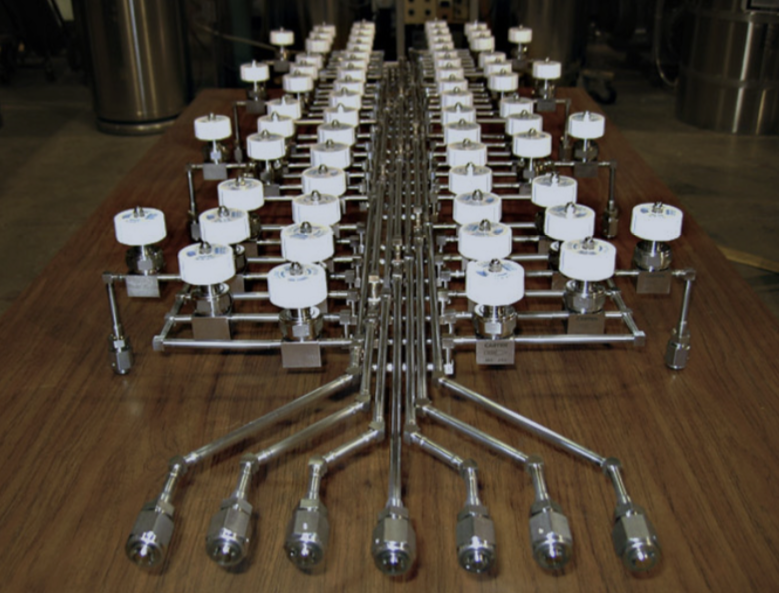
\includegraphics[width=0.9\textwidth]{cisc_GasAnalyzerSwitchyard.png}
\end{dunefigure}

The following lists three times the gas analyzer would be used.


\begin{enumerate}
\item Once the detector is installed and after the air atmosphere is eliminated from the cryostat to levels low enough to begin cooldown. This purge/gas recirculation process is detailed in Section~\ref{sec:fdgen-slow-cryo-install-ga}. Figure~\ref{fig:cisc_Phase1_purge_gas_recirculation} shows the evolution of the $\text{N}_2$, $\text{O}_2$, and $\text{H}_2\text{O}$ levels from gas analyzer data taken during the purge and recirculation stages of the DUNE \dword{35t} %Prototype P
phase 1 run.

\item Track trace $\text{O}_2$ and $\text{H}_2\text{O}$ contaminants from $\>$tens of ppb to hundreds of ppt. This is useful when other means of monitoring impurity levels (e.g., purity monitors, or \dshort{tpc} tracks) are not yet sensitive. Figure~\ref{fig:cisc_O2AnalyzerPrM2_HVRun1} shows a example plot of $\text{O}_2$ levels at the beginning of \dword{lar} purification from one of the later \num{35}\si{t} %Prototype 
\dword{hv} runs.

\item Monitor the tanker \dword{lar} delivery purity during cryostat filling. This tracks the impurity load on the filtration system and rejects any deliveries that do not meet specifications. Likely specifications for the delivered \dword{lar} are in the \SI{10}{ppm} range per contaminant.

\end{enumerate}

\begin{dunefigure}[Photo of a Switchyard Valve Assembly]{fig:cisc_Phase1_purge_gas_recirculation}
  {Plot of the O2, H2O, and N2 levels during the piston purge and gas recirculation stages of the 35 Ton Cryostat Phase 1 run}
  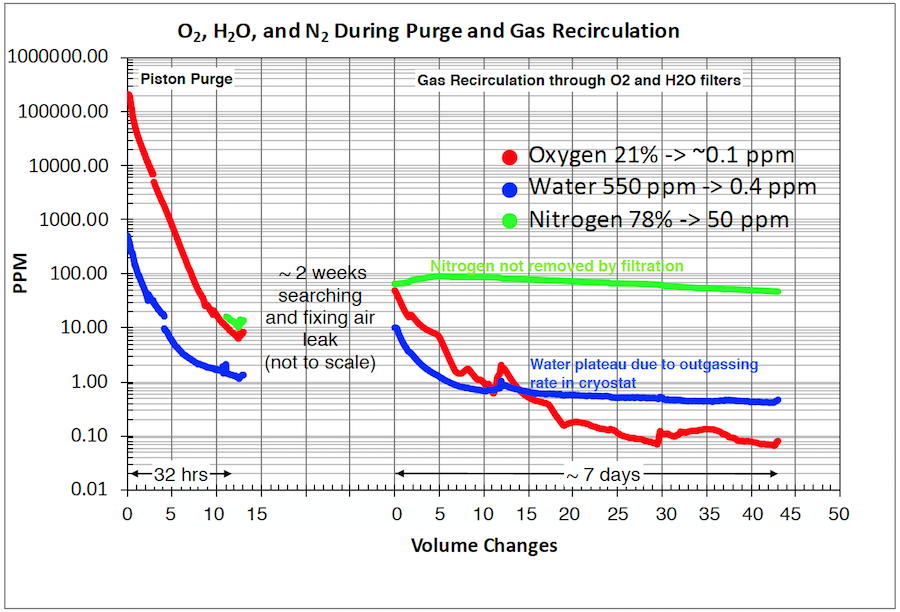
\includegraphics[width=0.7\textwidth]{cisc_Phase1_purge_gas_recirculation.png}
\end{dunefigure}

\begin{dunefigure}[Photo of a Switchyard Valve Assembly]{fig:cisc_O2AnalyzerPrM2_HVRun1}
  {O2 as measured by a precision O2 analyzer just after the 35T cryostat was filled with LAr, continuing with the LAr pump start and beginning of LAr recirculation through the filtration system. As the gas analyzer loses sensitivity, the purity monitor can pick up the impurity measurement. Note that the purity monitor is sensitive to both O2 and H2O impurities giving rise to its higher levels of impurity.}
  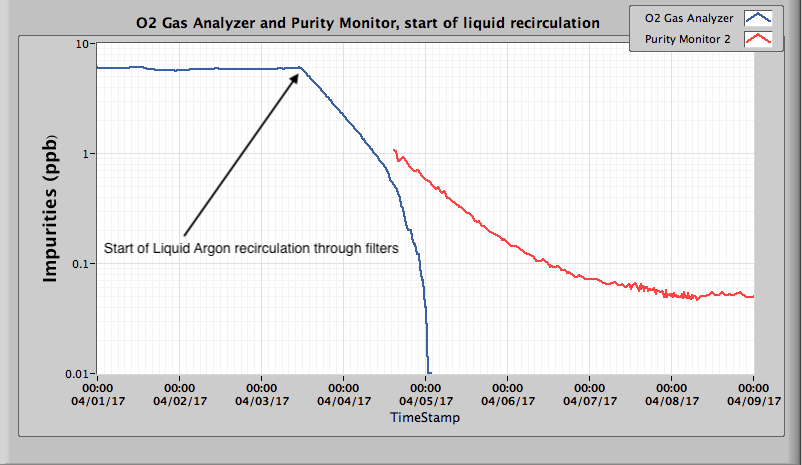
\includegraphics[width=0.7\textwidth]{cisc_O2AnalyzerPrM2_HVRun1.png}
\end{dunefigure}

Because any one gas analyzer covers only one contaminant species and \numrange{3}{4} orders of magnitude of range, several units are needed both for the three contaminant gases and to cover the ranges seen between  cryostat closure and the beginning of \dshort{tpc} operations:
\SI{20}{\percent} to $\lesssim 100$~ppt for $\text{O}_2$,
\SI{80}{\percent} to $\lesssim 1$~ppm for $\text{N}_2$, and
$\sim \SI{1}{\percent}$ to $\lesssim 1$~ppb for $\text{H}_2\text{O}$.
Because the total cost of these analyzers exceeds $\SI{100}[\textdollar]{k}$, we want to be able to  sample more than a single location or cryostat with the same gas analyzers. At the same time, the tubing run lengths from the sample point should be as short as possible to maintain a timely response for the gas analyzer. This puts some constraints on sharing devices because, for example, argon is delivered at the surface, so a separate gas analyzer may be required at the surface.

% \fixme{Do Gas Analyzers have ProtoDUNE design and results? Alan and Stephen say they weren't used as extensively at PDSP as at 35t, and "35t is also a prototype and has shown how gas analyzers can be used."}

%%%%%%%%%%%%%%%%%%%%%55 CAMERAS %%%%%%%%%%%%%%%%%%%%%%%%5
\subsection{Cameras}
% glenn, jim s, chuck
% same text in single and dual phase

Cameras provide direct visual information about the state of the
\dword{detmodule} during critical operations and when damage or unusual
conditions are suspected.  Cameras in the \dword{wa105} showed spray from cool-down
nozzles and the level and state of the \lar as it covered the \dword{crp} \cite{Murphy:20170516}.  A camera was
used in the Liquid Argon Purity Demonstrator
cryostat\cite{Adamowski:2014daa} to study \dword{hv} discharges in
\lar and in EXO-100 while a TPC was operating
\cite{Delaquis:2013hva}.  Warm cameras viewing \lar from a distance
have been used to observe \dword{hv} discharges in \lar in
fine detail \cite{Auger:2015xlo}.  Cameras are commonly used during
calibration source deployment in many experiments (e.g., the
\kamland ultra-clean system \cite{Banks:2014hra}).

In DUNE, cameras verify the stability, straightness,
and alignment of the hanging TPC structures during cool down and
filling; to ensure that no bubbling occurs near the \dwords{gp}
(\single) or \dwords{crp} (\dual); to inspect the
state of movable parts in the \dword{detmodule} (calibration devices, dynamic
thermometers); and to closely inspect parts of the TPC after any seismic activity or other unanticipated
event.  For these functions, a set of fixed
\textit{cold} cameras are used; they are permanently mounted at fixed points in the cryostat
for use during filling and commissioning, and a movable, replaceable
\textit{warm} inspection camera can be deployed through any free
instrumentation flange at any time during the life of the
experiment. 
% [GAHS: I commented out the table.] Table \ref{tab:fdgen-cameras-req} summarizes the requirements for the camera system.

Eleven cameras were deployed in \dword{pdsp} at the locations shown in Fig.~\ref{fig:pdsp-camera-locations}. They successfully provided views of the detector during filling and throughout the operation of the detector.

\begin{dunefigure}[Camera locations in \dword{pdsp}]{fig:pdsp-camera-locations}
  {A 3d view showing the locations of the 11 cameras in \dword{pdsp}.}
  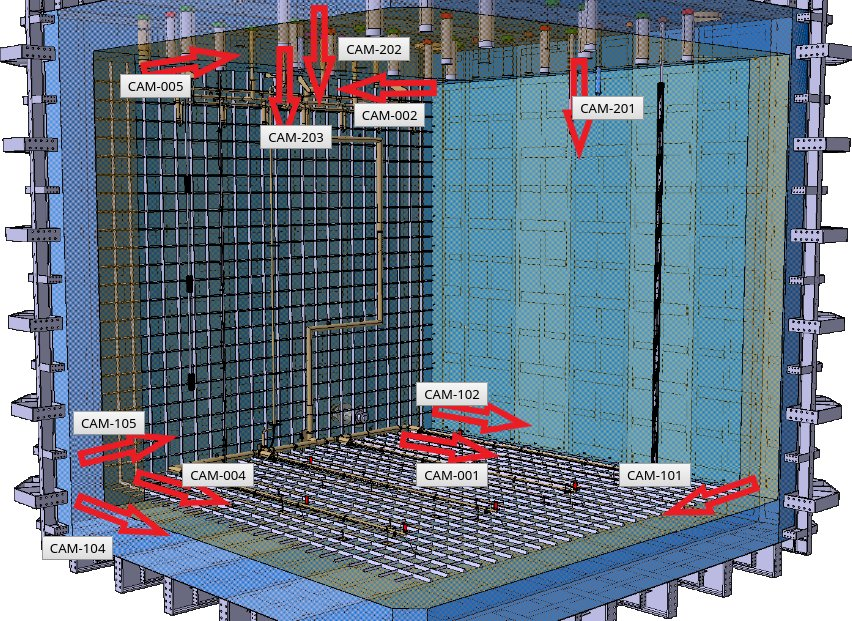
\includegraphics[width=0.6\textwidth]{pdsp-camera-locations-3d}%
\end{dunefigure}

The following sections describe the design considerations for both cold
and warm cameras and the associated lighting system. \dword{pdsp} camera system designs and performance are also discussed.  
The same basic
designs can be used for both the single and dual phase detectors.

% GAHS: I commented out the table
% \begin{dunetable}
% [Camera system requirements]
% {p{0.45\linewidth}p{0.50\linewidth}}
% {tab:fdgen-cameras-req}
% {Camera system requirements}   
%  Requirement & Physics Requirement Driver \\ \toprowrule
%  \multicolumn{2}{l}{\bf General} \\ \specialrule{1.5pt}{1pt}{1pt}
%  No component may contaminate the \lar{}. & High \lar purity is required for TPC operation. \\ \colhline
%  No component may produce bubbles in the liquid argon if the \dword{hv} is on. & Bubbles increase risk of \dword{hv} discharge. \\ \colhline
%  No point in the camera system shall have a field greater than \SI{15}{kV/cm} when the drift field is at nominal voltage. & Fields must be well below \SI{30}{kV/cm} to avoid risk of \dword{hv} discharge.\\ \colhline
% The camera system shall not produce measurable noise in any detector system. & Low noise is required for TPC operation. \\ \colhline
%  Cameras provide the viewing functionality as agreed upon with the other subsystems for viewing, as documented in the ICDs with the individual systems. \\ \toprowrule
% \multicolumn{2}{l}{\bf Cold cameras}\\ \specialrule{1.5pt}{1pt}{1pt}
% Minimize heat dissipation when camera not in operation. & Do not generate bubbles when \dword{hv} is on. \\ \colhline
% Longevity must exceed \num{18} months. & Cameras must function throughout cryostat filling and detector commissioning. \\ \colhline
% Frame rate \(\geq\SI{10}{\per s}\). & Observe bubbling, waves, detritus, etc. \\ \toprowrule
% \multicolumn{2}{l}{\bf Inspection cameras}\\ \specialrule{1.5pt}{1pt}{1pt}
% Keep heat transfer to \lar low when in operation. & Do not generate bubbles, some use cases may require operation when \dword{hv} is on. \\ \colhline
% Deploy without exposing \lar to air. & Keep \lar free of N2 and other electronegative contaminants. \\ \colhline
% Camera enclosure must be replaceable. & Replace broken camera, or upgrade, throughout life of experiment. \\ \colhline
% {\bf Light emitting system} \\ \colhline
% No emission of wavelengths shorter than \(\SI{400}{nm}\) & Avoid damaging \dword{tpb} waveshifter. Note emitted wavelength shortens significantly with temperature. \\ \colhline
% Longevity must exceed \num{18} months. & Lighting for fixed cameras must function throughout cryostat filling and detector commissioning. \\ \colhline
% \end{dunetable}

%\fixme{Cameras intro: GAHS -- do we want to keep the separate, lower-level table of requirements for cameras?  I think we have to put key high-level requirements in the requirements table in the Requirements section, and drop this table. [dropped, but need to check for things to add to Requirements]}

%%%%%%%%%%%%%%%%%%%%%%%%%%%%%%%%%%%%%%%
\subsubsection{Cryogenic Cameras (Cold)}

The fixed cameras
monitor the following items during filling:
\begin{itemize}
\item Positions of corners of \dword{apa} or \dword{crp}, \dword{cpa} or cathode, \dwords{fc}, \dwords{gp} (\SI{1}{mm} resolution);
\item Relative straightness and alignment of \dword{apa}/\dword{crp}, \dword{cpa}/cathode, and \dword{fc} (\(<\sim\SI{1}{mm}\));
\item Relative positions of profiles and endcaps (\SI{0.5}{mm} resolution);
\item \lar surface, specifically, the presence of bubbling or debris.
\end{itemize}


% GAHS: I commented out the past performance discussion because the PDSP cameras performed so well.
% There are published articles and unpublished presentations describing
% completely or partially successful operation of low-cost,
% off-the-shelf \dword{cmos} cameras in custom enclosures immersed in cryogens.
% (e.g., EXO-100: \cite{Delaquis:2013hva}; DUNE \dword{35t} test
% \cite{McConkey:2016spe}; \dword{wa105}: \cite{Murphy:20170516}.)  Generally
% it is reported that such cameras show poor performance and ultimately
% fail to function below some temperature of order \SIrange{150}{200}{K}, but some report that their cameras recover fully after
% being stored (not operated) at temperatures as low as \SI{77}{K} and
% then brought up to minimum operating temperature.

% However, as with photon sensors, experience has also shown that it is
% non-trivial to ensure reliable and reproducible mechanical and
% electrical integrity of such cameras in the cryogenic environment 
% (e.g., \cite{McConkey:2016spe} and
% \cite{Valencia-Rodriquez:20180130}).  Off-the-shelf cameras and camera
% components are generally only specified by the vendors and original
% manufacturers for operation down to \SI{-40}{\celsius} or \SI{-50}{\celsius}.
% In addition, many low-cost cameras use digital interfaces not intended
% for long distance deployment, such as USB (\(2\sim\SI{5}{m}\)) or CSI (circuit
% board scale), leading to signal degradation and noise problems.

One design for the DUNE fixed cameras uses an enclosure similar to
the successful EXO-100 design \cite{Delaquis:2013hva}, which was also
successfully used in the Liquid Argon Purity Demonstrator
and \dword{pdsp} (see Figure~\ref{fig:gen-fdgen-cameras-enclosure}). Cameras 101, 102, 104, and 105, shown in Fig.~\ref{fig:pdsp-camera-locations}, use this enclosure.
A thermocouple in the enclosure allows temperature monitoring, and a heating element provides temperature control.  
SUB-D connectors are used at the cryostat flanges and the camera enclosure for signal, power, and control connections.
% The enclosure is connected to a stainless steel gas line to allow it to be flushed with argon gas at low enough pressure to prevent liquification, using the same design as the gas line for the beam plug tested in the \dword{35t} \dword{hv} test and in \dword{protodune}.  
%The camera transmits its video signal using either a composite video signal over shielded coax or Ethernet over optical fiber.  Most importantly, the DUNE \dword{cisc} consortium must work with vendors to design camera circuit boards that are robust and reliable in the cryogenic environment.

\begin{dunefigure}[A camera enclosure]{fig:gen-fdgen-cameras-enclosure}
  {Top left: a CAD exploded view of a vacuum-tight camera enclosure suitable for cryogenic applications \cite{Delaquis:2013hva}.
    (1) quartz window, (2 and 7) copper gasket, (3 and 6) flanges, (4) indium wires, (5) body piece, (8) signal \fdth.
    Top right: two of the \dword{pdsp} cameras using a stainless steel enclosure. 
    Bottom left: one of the \dword{pdsp} cameras using acrylic enclosure.
    Bottom right: a portion of an image taken with \dword{pdsp} camera 105 showing a purity monitor mounted outside the \dword{apa} on the beam left side. This photo was taken with \dword{pdsp} completely filled.
  }
  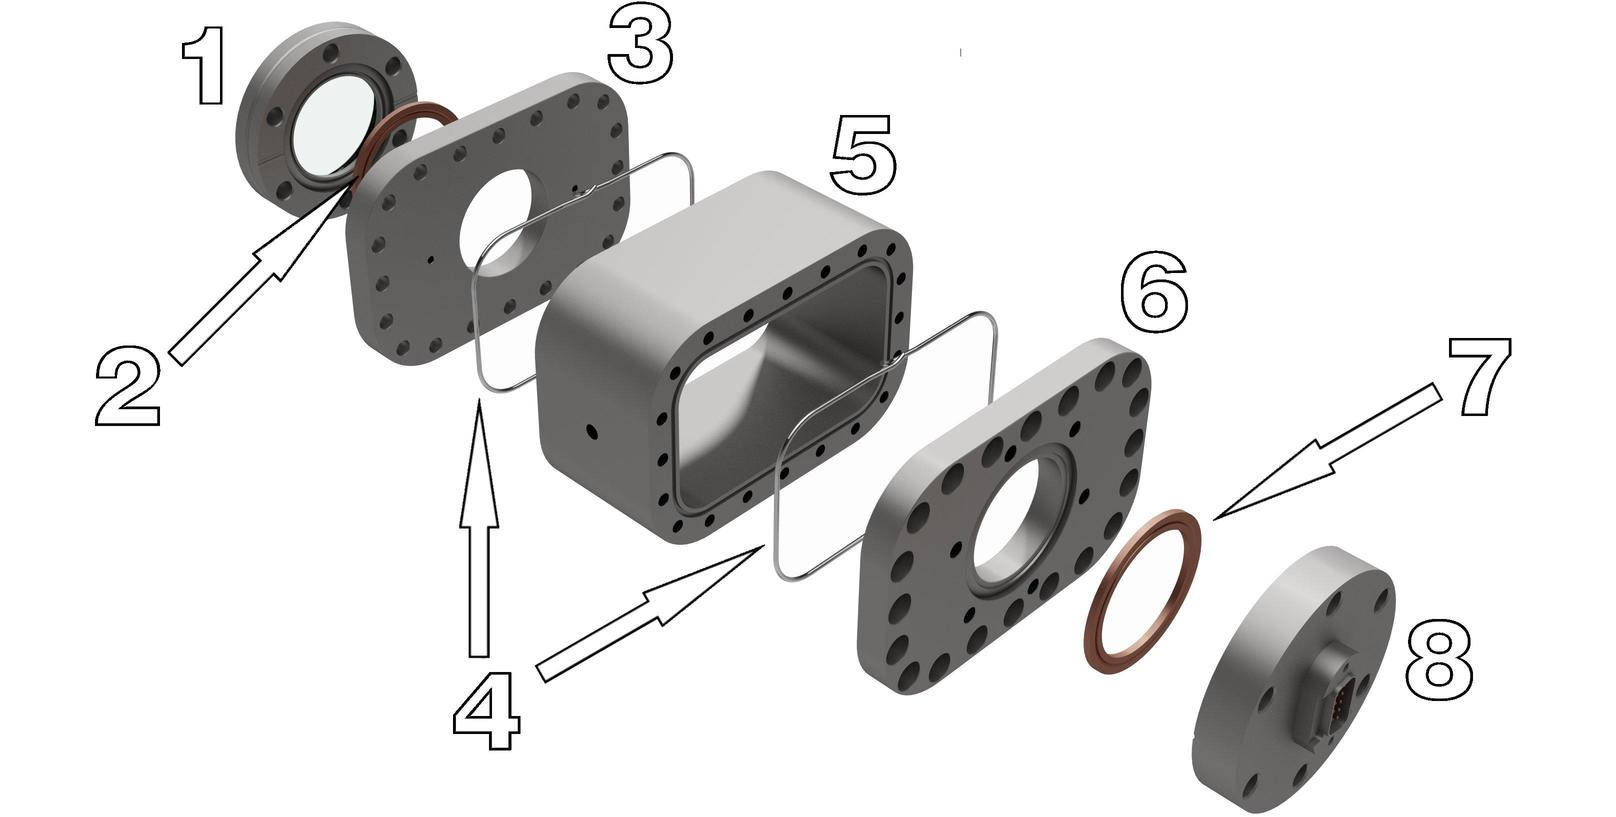
\includegraphics[width=0.4\textwidth]{exo100-camera-case}%
  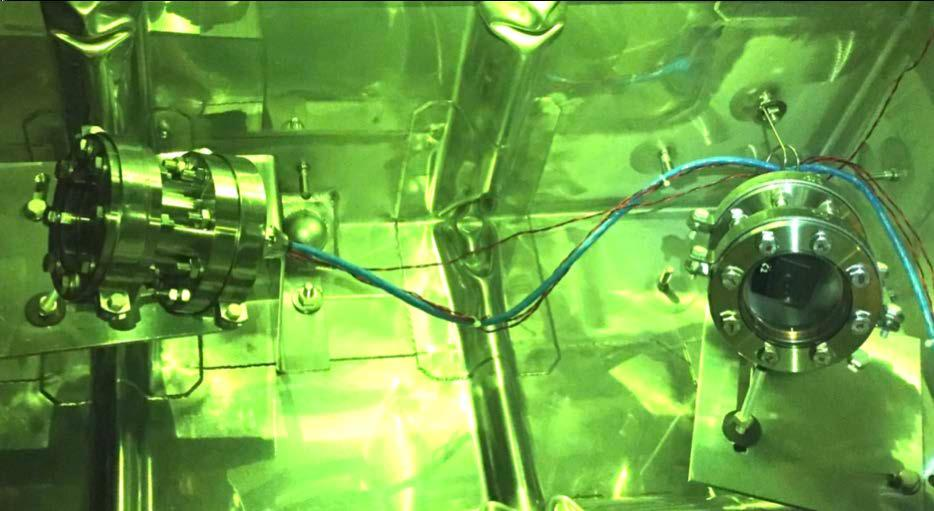
\includegraphics[width=0.4\textwidth]{edgar-cameras}\\
  \hfill 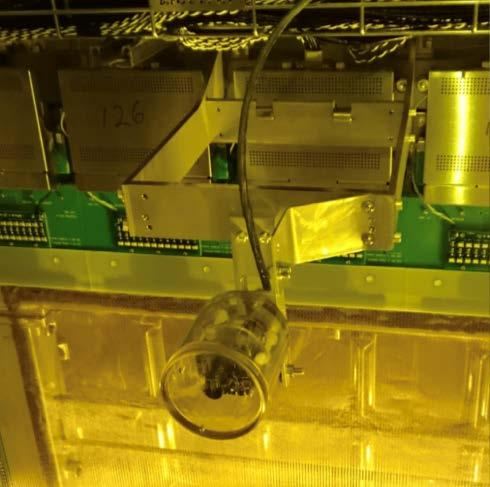
\includegraphics[width=0.22\textwidth]{bo-camera}%
  \hfill 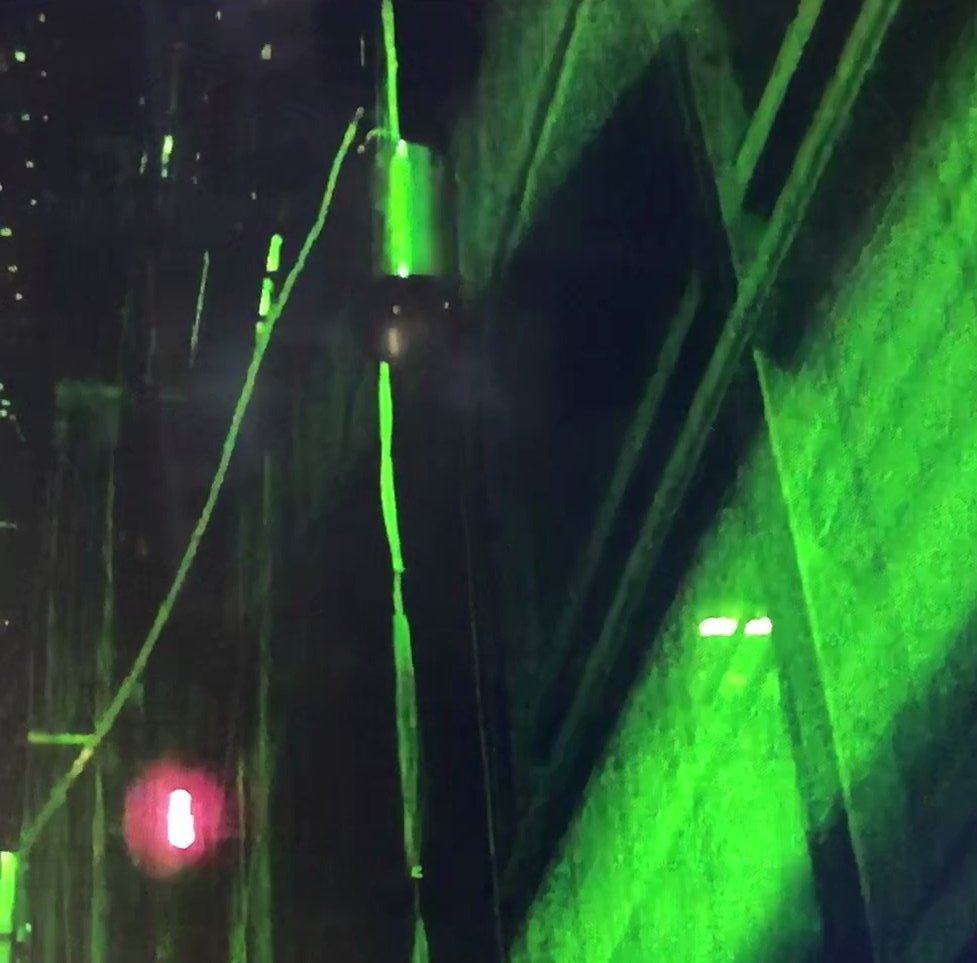
\includegraphics[width=0.22\textwidth]{camera-105-purmon-orig-rot-crop}%
  \hfill
\end{dunefigure}

An alternative design uses an acrylic enclosure.
This design was used successfully in \dword{pdsp} (see Figure~\ref{fig:gen-fdgen-cameras-enclosure}, bottom left). Cameras 001, 002, 004, and 005 shown in Fig.~\ref{fig:pdsp-camera-locations} use acrylic enclosures. 
All operate successfully, including those at the bottom of the cryostat.


%%%%%%%%%%%%%%%%%%%%%%%%%%%%%%%%%%%%%%%%%%%%%%%5
\subsubsection{Inspection Cameras (Warm)}

The inspection cameras are intended to be as versatile as possible.
However, the following locations have been identified as likely
to be of interest:
\begin{itemize}
\item Status of \dword{hv} \fdth and cup;
\item Status of \dword{fc} profiles, endcaps (\SI{0.5}{mm} resolution);
\item $y$-axis deployment of calibration sources;
\item Status of thermometers, especially dynamic thermometers;
\item \dword{hv} discharge, corona, or streamers on \dword{hv} \fdth, cup, or \dword{fc};
\item Relative straightness and alignment of \dword{apa}/\dword{crp}, \dword{cpa}/cathode, and \dword{fc} (\SI{1}{mm} resolution);
\item Gaps between \dword{cpa} frames (\SI{1}{mm} resolution);
\item Relative position of profiles and endcaps (\SI{0.5}{mm} resolution);
\item Sense wires at the top of outer wire planes in \single \dword{apa} (\SI{0.5}{mm} resolution).
\end{itemize}

Unlike the fixed cameras, the inspection cameras must operate only as
long as inspection lasts; the cameras can be replaced in case of failure.  It
is also more practical to keep the cameras continuously warmer than
 \SI{-150}{\celsius} during deployment; this allows using %and therefore we willhave 
commercial cameras more easily, e.g., %.  For example, we could deploy 
the same model camera used successfully to observe discharges
in \lar from \SI{120}{cm} away \cite{Auger:2015xlo}.

\begin{dunefigure}[Inspection camera design]{fig:gen-fdgen-cameras-movable}
  {Left: An overview of the inspection camera design using a sealed deployment system opening directly into the cryostat. Right: A photo of the \dword{pdsp} warm inspection camera acrylic tube, immediately before installation; the acrylic tube is sealed with an acrylic dome at the bottom and can be opened at the top.}
  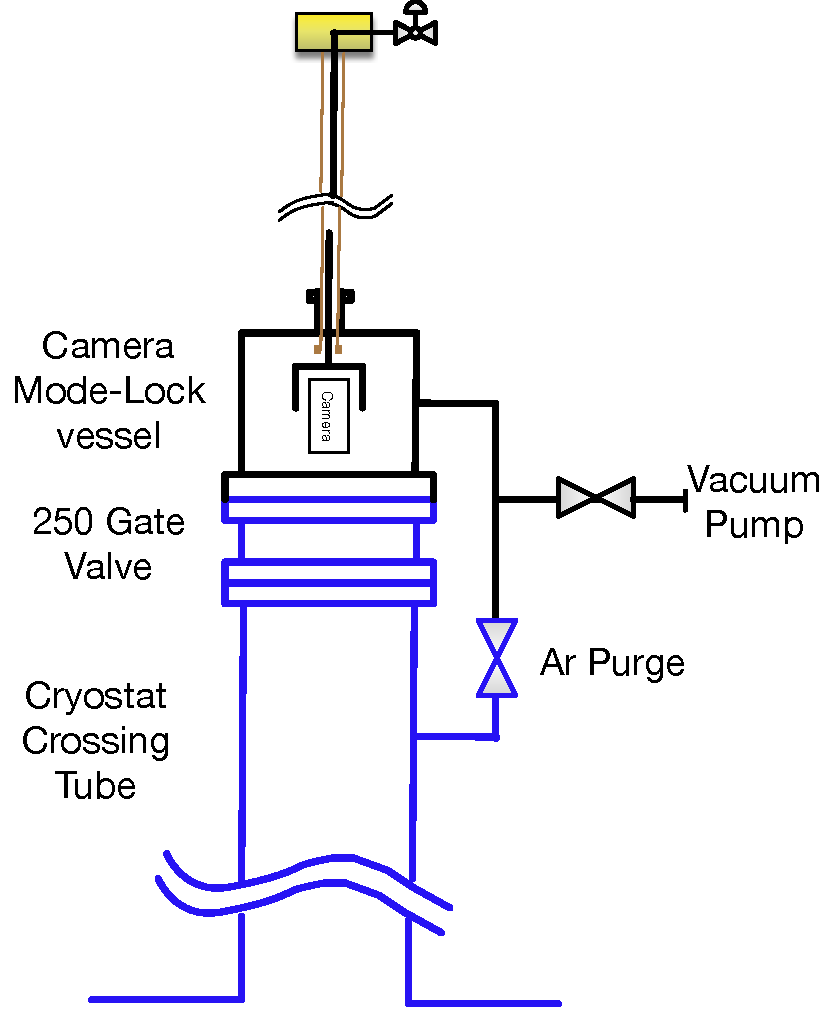
\includegraphics[height=0.3\textheight]{Camera-Sketch}%
  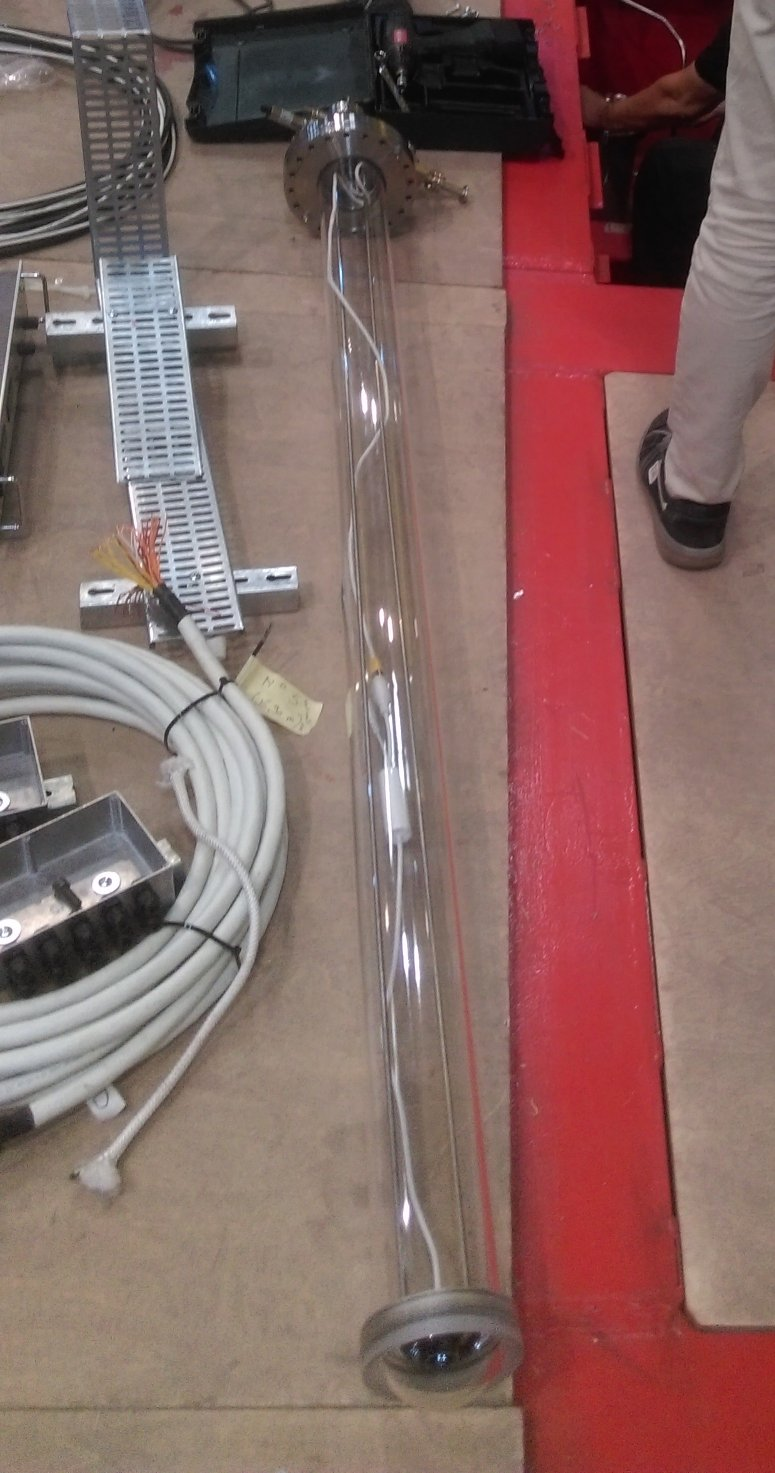
\includegraphics[height=0.3\textheight]{cisc-pdsp-camera-tube}%
\end{dunefigure}

The design for the inspection camera system uses the same basic
enclosure design as for cold cameras, but they are mounted on an insertable
fork \fixme{This could be clearer. "...an insertable fork" would be clearer if we knew where it was to be inserted. So try something like this: "...mounted on a fork so the camera can be inserted into ? using a design similar to the dynamic temperature probes."} using a design similar to the dynamic temperature probes. See
Figure~\ref{fig:gen-fdgen-cameras-movable}(left) and
Figure~\ref{fig:fd-slow-cryo-sensor-mount}.  The entire system is sealed to
avoid contamination with air \fixme{This sounds like you are trying to avoid contaminating the camera with air. I suggest omitting this sentence. Add to the following sentence to clarify where the contamination may occur. So "To avoid contamination of ?, the camera can only be deployed..."} . To avoid contamination, the
camera can only be deployed through a \fdth equipped with a gate
valve and a purging system, similar to the one used in the vertical axis
calibration system at \kamland~\cite{Banks:2014hra}. The entire system
is  purged with pure argon gas before the gate valve is opened.

Motors above the flange allow the fork to be rotated and moved vertically to position the camera. 
 A chain drive system with a motor
mounted on the end of the fork allows the camera assembly to tilt, 
creating a point-tilt mount that can be moved vertically.
With the space above the cryostat flanges and the
thickness of the cryostat insulation, cameras can be moved vertically up to
\SI{1}{m} inside the cryostat.
% In the event that it
% becomes necessary to deploy a camera more deeply, we would have the
% option of building a a cable deployment system or a multi-pole
% deployment system similar to the KamLAND full-volume calibration
% system\cite{Busenitz:2009ac}, but this is not currently part of the
% baseline design.
The motors for rotation and vertical motion are outside the sealed
volume, coupled mechanically using ferrofluidic seals, thus reducing any risk of
contamination and allowing manual rotation of the vertical
drive in the event of motor failure.  

An alternative design was demonstrated in \dword{pdsp}. In this design, the warm camera is contained inside a gas-tight acrylic tube inserted into the feedthrough, so a gate valve or a gas-tight rotatable stage is not needed, and the warm cameras can be removed for servicing or upgrade at any time. Fig.~\ref{fig:gen-fdgen-cameras-movable}(right) shows an acrylic tube enclosure and camera immediately before deployment. These acrylic tube enclosures for removable cameras were deployed at the positions marked 201, 202, and 203 in Fig.~\ref{fig:pdsp-camera-locations}; they operated successfully in \dword{pdsp}. Cameras with fisheye lenses were used in these tubes during initial operation; we plan to use other cameras during post-beam running.

To finalize and validate these designs for DUNE, we will continue prototyping and testing, focusing particularly on longevity and pressure resistance.


%%%%%%%%%%%%%%%%%%%%%%%%%%%%%%%%%%%%%%%
\subsubsection{Light-emitting system}
%%% same text as dual-phase
The light-emitting system uses \dwords{led} that can illuminate the interior \fixme{of what?} with selected
wavelengths (IR and visible) that cameras can detect.  Performance criteria for the light-emission system include the efficiency with which the cameras can detect the light and the need to avoid
adding heat to the cryostat. Very high-efficiency
\dwords{led}   
help reduce heat generation; one \SI{750}{nm} \dword{led} \cite{lumileds-DS144-pdf}
has a specification equivalent to
\SI{33}{\%} conversion of electrical input power to light.

% CEL: 1W electrical gives 425mW blue flux, power limit from SMD package thermal resistance of 8C/W to have max 1C increase at LED. CREE Xlamp XP-E model

While data on how well \dwords{led} perform at cryogenic temperatures is sparse,
some studies of NASA projects~\cite{Carron:2017zzz} 
indicate that \dword{led} are more efficient at low temperatures
and that emitted wavelengths may change, particularly for blue \dwords{led}.
These wavelength changes would not affect illumination, however, because
to avoid degradation of wavelength-shifting materials in the \dword{pds},
such short wavelength \dwords{led} would not be used.

\begin{dunefigure}[Example schematic for LED chain]{fig:cisc-LED}
  {Example schematic for LED chain, allowing failure tolerance and two LED illumination spectra.}
  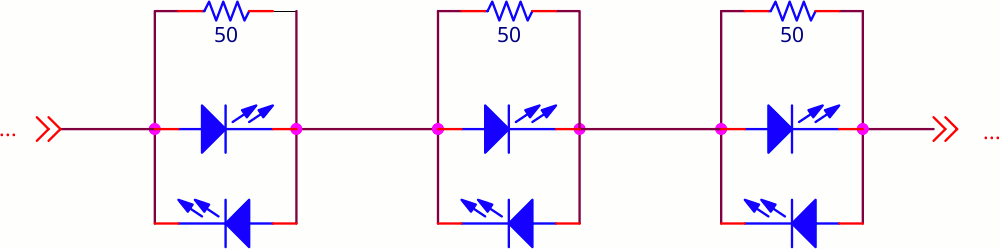
\includegraphics[width=0.6\textwidth]{cisc_led.png}
\end{dunefigure}

A chain of \dwords{led} connected in a series and driven with a
constant-current circuit could be set up, with each
\dword{led} paired in parallel with an opposite polarity \dword{led} and a resistor
(see Figure~\ref{fig:cisc-LED}).
This allows two different wavelengths of illumination using a single chain simply by changing the direction of the drive current. This allows continued use of an \dword{led} chain even if individual \dwords{led} fail.

The \dwords{led} should be placed as a ring of light around the outside of each
camera, pointing in the same direction as the lens, to 
illuminate the part of the \dword{detmodule} lying within the camera's field of
view. Commercially available \dwords{led} can be obtained with
a range of angular spreads that can be matched to the needs of the
cameras without additional optics.


%%%%%%%%%%%%%%%%%% CRYOGENIC TEST FACILITY %%%%%%%%%%%%%%%%%%%%
\subsection{Cryogenic Test Facility}
% same for SP and DP
% alan h

The Cryogenic Test Facility provided access to small (< \SI {1} {ton}) to intermediate (~\SI {5} {ton}) volumes of purified "TPC-grade" \dword{lar}. Hardware that requires this high purity liquid includes any device intending to drift electrons for millisecond periods. Not all devices need this high purity \dword{lar} but may need a relatively large volume for the necessary prototyping environments. A relatively fast turn-around time of approximately a week is needed for short prototyping runs. 

\begin{dunefigure}[Photo of a Switchyard Valve Assembly]{fig:cisc_PAB_photo}
  {Photo of PAB Cryogenic Test Facility at FNAL.}
  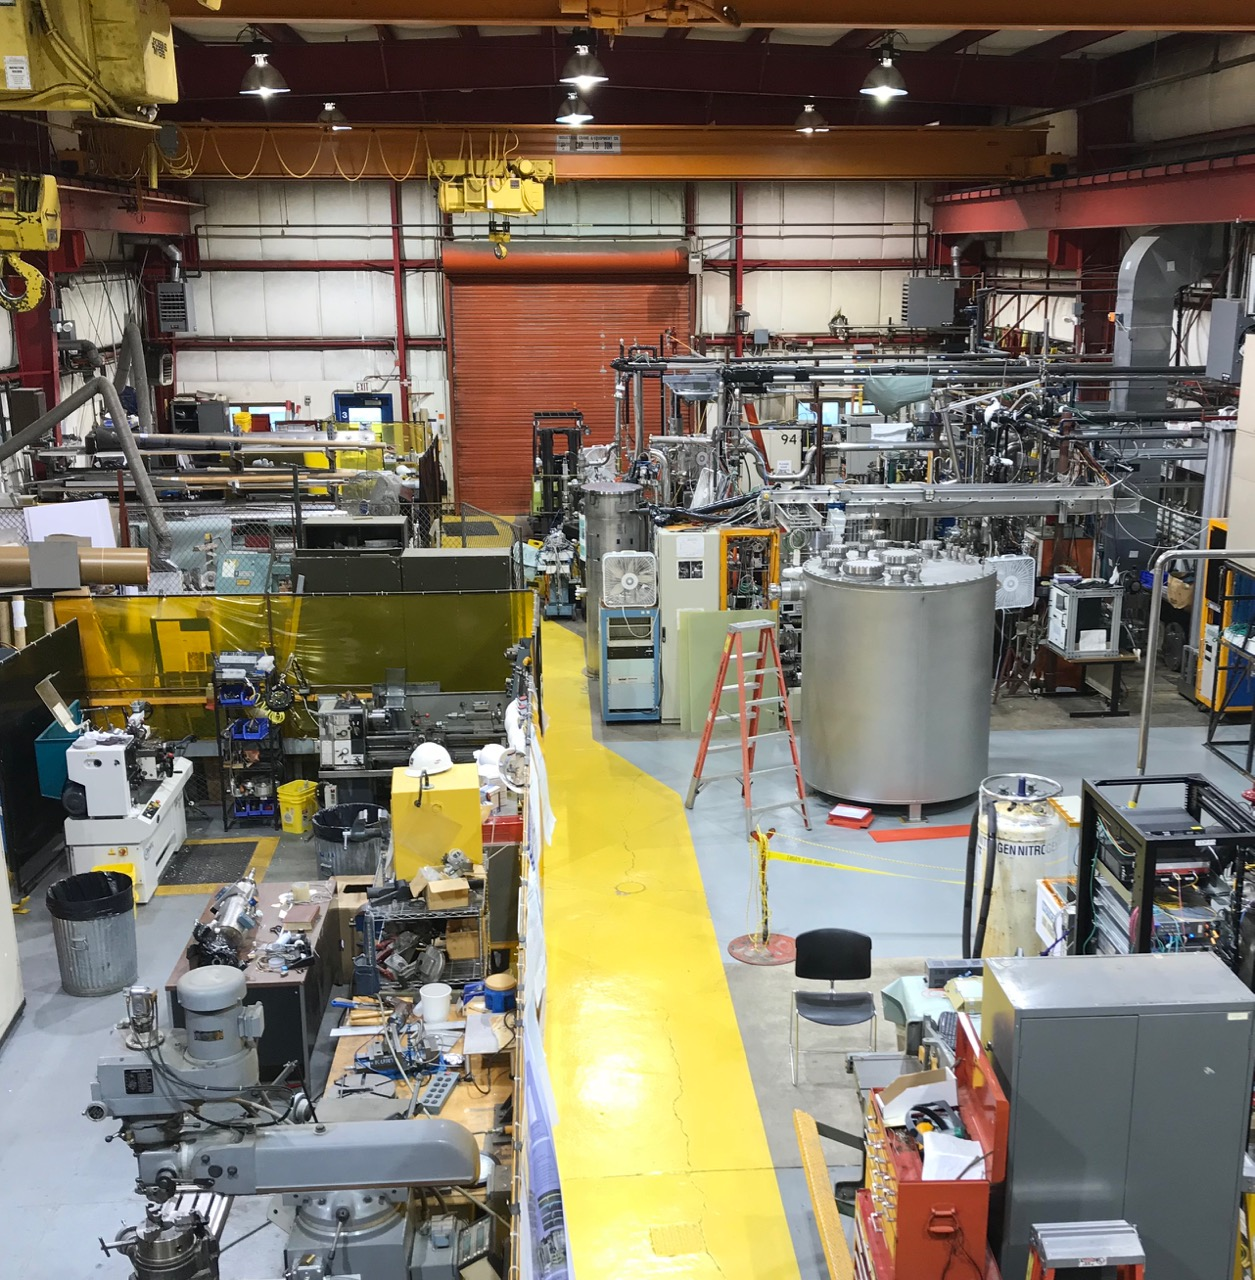
\includegraphics[width=0.9\textwidth]{cisc_PAB_photo.jpg}
\end{dunefigure}

Figure ~\ref{fig:cisc_PAB_photo} is a photo of the PAB facility at FNAL showing the ICEBERG \SI {3000} {liter} cryostat being readied for outfitting. This cryostat serves as a fast turn-around facility for the DUNE Cold Electronics Small TPC test facility. Also in the photo is a technical shop (left bottom) as well Tall Bo (\SI {450} {liter}), Blanche (\SI {500} {liter}), and Luke (\SI {250} {liter}) cryostats in the background. All these cryostats are available for outside use. In the recent past, Blanche has been used for \dword{hv} studies, Tall Bo for Photon Detector studies, and Luke for the material test stand work. These studies have contributed to the design and testing of ProtoDUNE \dword{sp} components.



%%%%%%%%
\section{Slow Controls}
% same for SP and DP

The slow controls system collects, archives, and displays data from
a broad variety of sources and provides real time status, alarms, and warnings for detector operators. Slow controls also provide control for some components of the detector systems such as \dword{hv} systems, \dword{tpc} electronics, and photon detector systems. Data is acquired via network interfaces.  Figure~\ref{fig:gen-slow-controls-diagram} shows connections between major parts of the slow controls system and other systems. Hardware, Infrastructure, and Software are the three main components of the slow controls system, each of which are described in this section.

\begin{dunefigure}[Slow Controls connections and data]{fig:gen-slow-controls-diagram}
{Typical slow controls system connections and data flow}
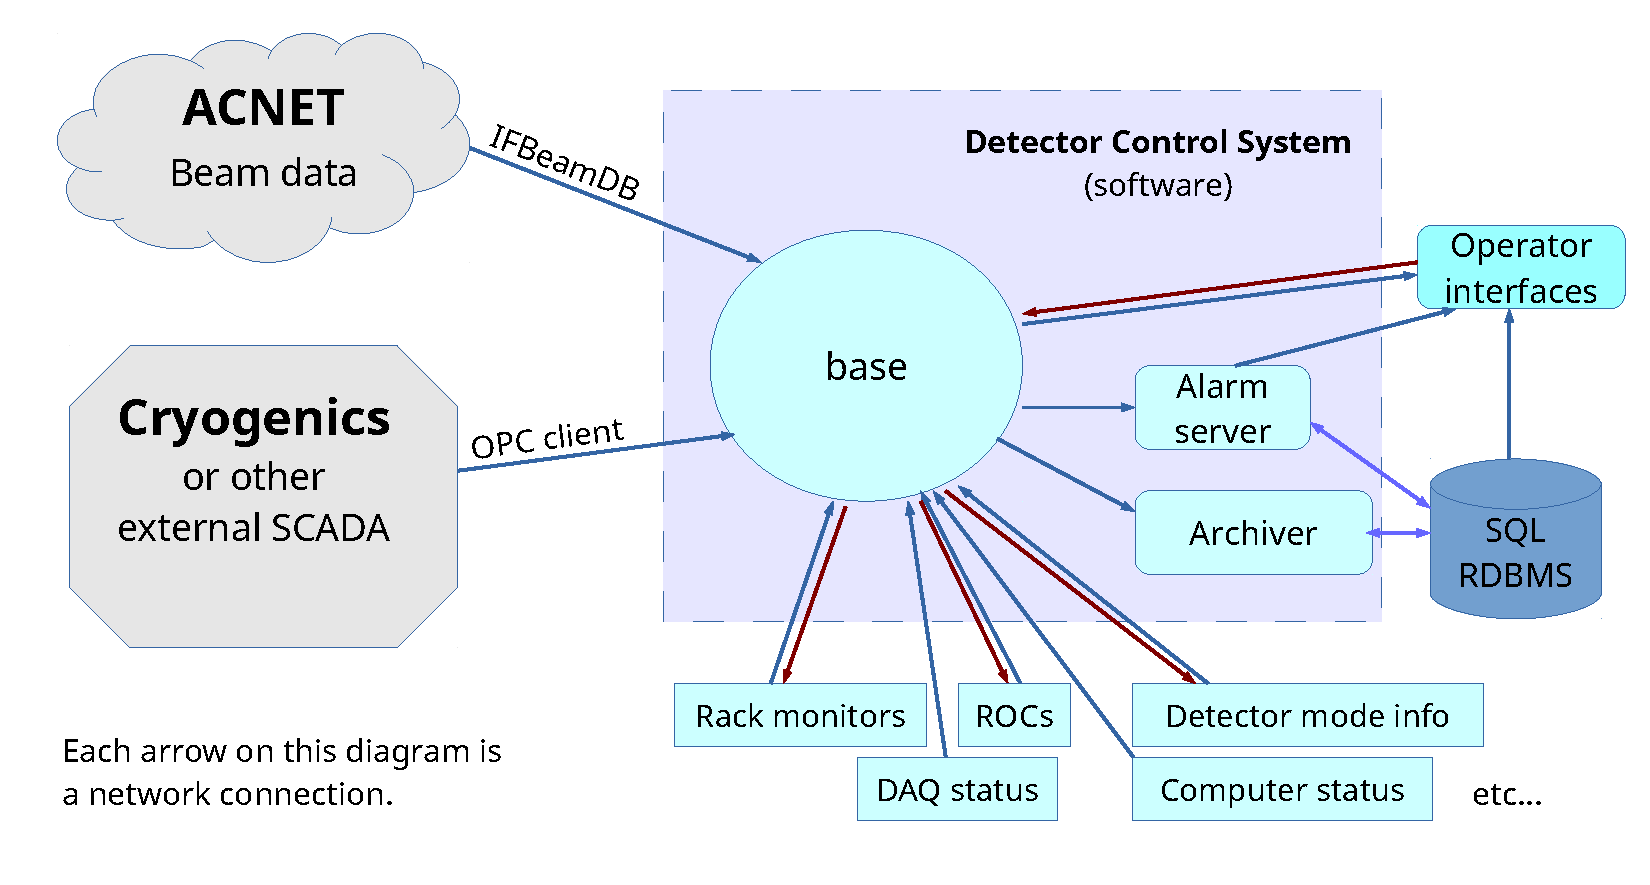
\includegraphics[width=0.7\textwidth]{cisc_slow-controls-diagram}
\end{dunefigure}

The \dword{pdsp} detector control system\cite{pdspdcs_proc} fully met the requirements for operating \dword{pdsp}. Section \ref{sec:cisc-slow-control-pdsp} provides a short description of the \dword{pdsp} slow controls and its performance.

%%%%%%%%%%%%%%%%%%%%%%%%%%%%%%%%%%%
 \subsection{Slow Controls Hardware}
\label{sec:fdgen-slow-cryo-hdwr}

A modest amount of dedicated hardware is envisioned for slow controls, largely for rack monitoring. Additionally, slow controls will always require a small amount of dedicated network and
computing hardware as described below. Slow controls also relies on common
infrastructure as described in
Section~\ref{sec:fdgen-slow-cryo-slow-infra}.

\subsubsection{Dedicated Monitoring Hardware}
Every rack (including those in the \dword{cuc}) should have dedicated hardware to monitor rack parameters like rack protection system, rack fans, rack air temperatures, thermal interlocks with power supplies, and any interlock bit status monitoring needed for the racks. For the racks in the \dword{cuc} server room, this functionality is built into the proposed water cooled racks, as already in place at ProtoDUNE.  For the racks on the detector itself, the current plan is to design and install a custom-built 1U rack-mount enclosure containing a single-board computer to control and monitor various rack parameters. Such a system has been successfully used in MicroBooNE. The design is being improved for the short-baseline near detector (SBND) experiment (see Figure~\ref{fig:slow-controls-rack-box}). Other slow controls hardware include interfacing cables like adapters for communication and debugging and other specialized cables like GPIB or National Instruments cables. The cable requirements must be determined in consultation with other groups once hardware choices for various systems are finalized.

\begin{dunefigure}[Rack monitoring box prototype being developed for the Short-Baseline Near Detector (SBND) experiment; based on the original design from MicroBooNE.]{fig:slow-controls-rack-box}
{Rack monitoring box prototype in development for the short-baseline near detector (SBND) experiment based on the original design from MicroBooNE.}
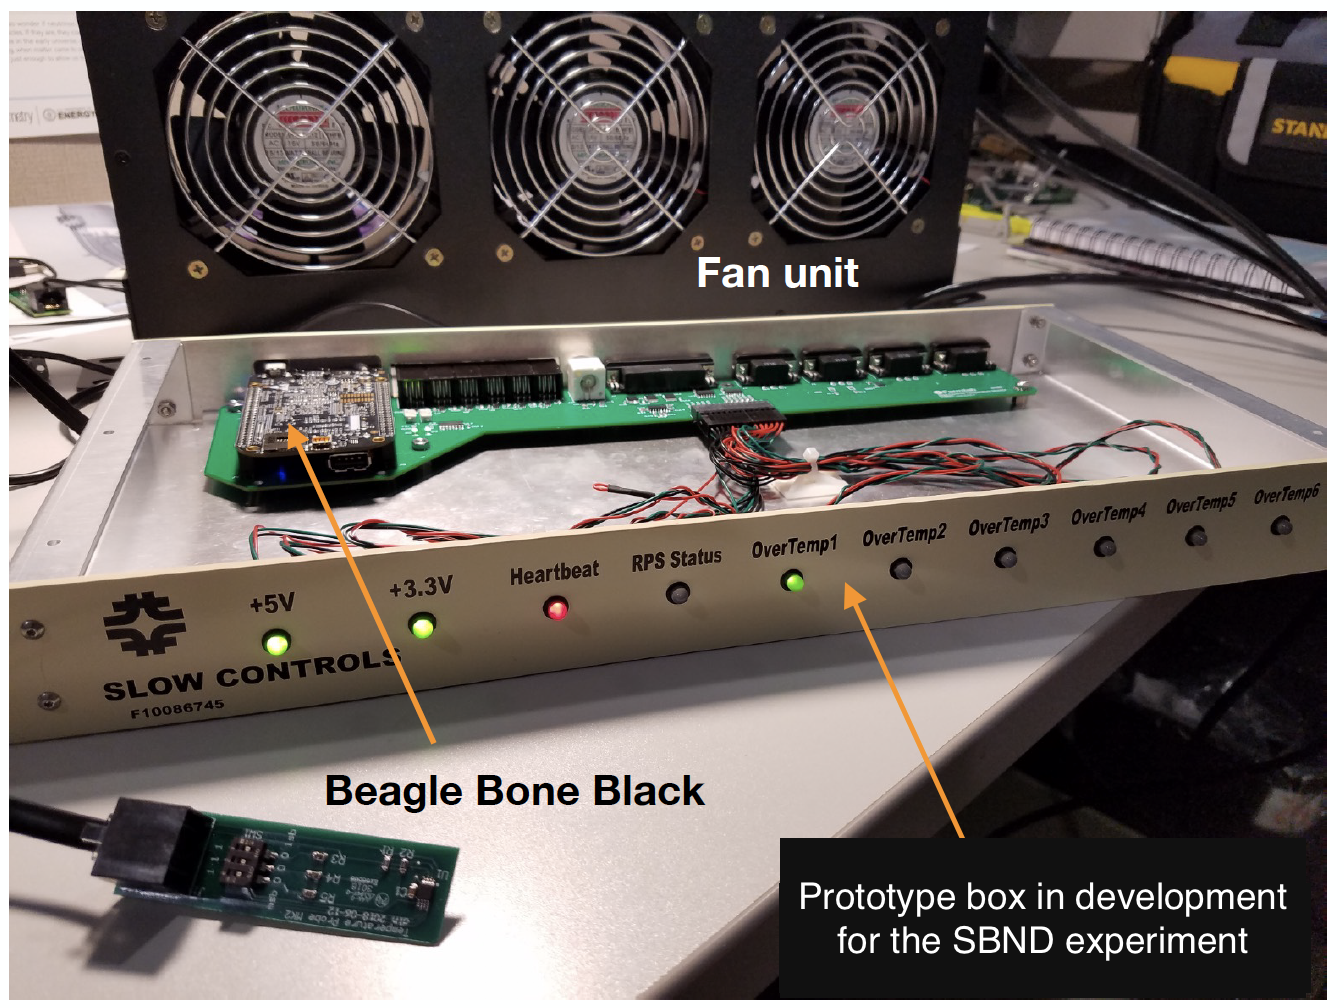
\includegraphics[width=0.6\textwidth]{cisc-slow-controls-rackbox.png}
\end{dunefigure}


% % % % Alec
\subsubsection{Slow Controls Network Hardware}
\label{sec:fdgen-slow-cryo-slow-network}
The slow controls data originates from the cryogenic instrumentation and from other systems as listed in Table~\ref{tab:gen-slow-quant}. This data is collected by software running on servers
(Section~\ref{sec:fdgen-slow-cryo-slow-compute})
housed in the underground data room in the \dword{cuc},
where data is archived in a central \dword{cisc} database.
The instrumentation data is transported over
conventional network hardware from any sensors located in the cryogenic
plant.  However, the readouts that are in the racks on top of the
cryostats must be cautious about grounding and noise.  Therefore, each
rack on the cryostat has a small network switch that sends
any network traffic from that rack to the \dword{cuc} via a fiber transponder.
This is the only network hardware specific to slow controls and will be provided by the laboratory's general computing infrastructure managed by project \dword{tc}. The network infrastructure requirements are described in
Section~\ref{sec:fdgen-slow-cryo-slow-infra}.

% % % % Alec
\subsubsection{Slow Controls Computing Hardware}
\label{sec:fdgen-slow-cryo-slow-compute}
Two servers (a primary server and a replicated backup) suitable for the relational database discussed
in Section~\ref{sec:fdgen-slow-cryo-sw} are located in the \dword{cuc} data
room, with an additional
two servers to service the \dword{fe} monitoring interface; such service would include assembling dynamic \dword{cisc} monitoring web pages from adjacent
databases.  Another server will be needed to run back-end I/O.  Any special purpose software, such as iFix used by the cryogenics experts, would
also run here. One or two additional servers should accommodate these programs.
% (The exact number of iFix machines will be determined based
% on input from the LBNF cryogenics experts.)
Replicating this setup on a per-module basis would make commissioning and independent operation easier, accommodate different module
design (and the resulting differences in database tables), and ensure
sufficient capacity.  These four sets of networking hardware would fit tightly into one rack or very comfortably into two. Using the requirements from \dword{cisc}, the \dword{daq} consortium will provide the cost estimates for servers and racks. 

% % % % Alec and Sowjanya
%% \subsubsection{Slow Controls Signal Processing Hardware}
%% Dropped because slow controls scope is defined not to include it.
%% (Signal processing should be within the scope of the hardware
%% generating the signal -- and so should digitization, for that matter.)
%%
%% N.B. The ``laundry list of Things to Be Monitored'' is in
%% \ref{sec:fdgen-slow-cryo-quant}



%%%%%%%%%%%%%%%%%%%%%%%%%%%%%%%%%%%
% Alec
\subsection{Slow Controls Infrastructure}
\label{sec:fdgen-slow-cryo-slow-infra}

The data rate will be in the range of tens of kilobytes per second, given the total number of slow controls quantities and the update rate  
(see Section~\ref{sec:fdgen-slow-cryo-quant}), placing minimal demands
on local network infrastructure.
Network traffic out of \surf to \fnal will primarily be database calls
to the central \dword{cisc} database, either from monitoring applications or from
database replication to the offline version of the \dword{cisc} database.  This
traffic requires little bandwidth, so the proposed general purpose
links both out of the mine and back to \fnal can accommodate the traffic.

Up to two racks of space and appropriate power and cooling are
available in the \dshort{cuc}'s \dword{daq} server room for \dword{cisc} use.
Somewhat less space than that is currently envisioned, as described in Section
\ref{sec:fdgen-slow-cryo-slow-compute}.

%%%%%%%%%%%%%%%%%%%%%%%%%%%%%%%%%%
% Sowjanya
\subsection{Slow Controls Software}
\label{sec:fdgen-slow-cryo-sw}
%\fixme{SG: does this need any updating based on presentations from Glenn/Alec at the Sept. Collaboration meeting? GAHS: I don't think so. PDSP DCS citation added. SG: okay, taking it out. I agree.}
% same for SP and DP

To provide complete monitoring and control of detector subsystems, the slow controls software includes the following components:
%
\begin{itemize}
 \item{Control systems base} that performs input and output operations
  and defines processing logic, scan conditions, alarm conditions,
  archiving rate, etc. \fixme{Either indicate this is a partial list at the beginning or provide the complete list. Eliminate the "etc."} ;
 \item{Alarm server} that monitors all channels and sends alarm
  messages to operators; 
 \item{Data archiver} that performs automatic sampling and storage of
  values for history tracking;
 \item{Integrated operator interface} that provides display panels for
  controls and monitoring.
\end{itemize}

An additional requirement for the software is the ability to indirectly
interface with external systems (e.g., cryogenics control
system) and databases (e.g., beam database) to export data into
slow controls process variables (or channels) for archiving and status
displays. This allows us to integrate displays and warnings into one
system for the experiment operators, and %to provide 
provides integrated
archiving for sampled data in the archived database. As one possibility, an input output controller (IOC) running on a central \dword{daq}
server could provide soft channels for these data.
Figure~\ref{fig:gen-slow-controls-diagram} shows a typical workflow of a
slow controls system.

The key features of the software require highly evolved software designed to manage real-time data exchange, scalable
to hundreds of thousands of channels sampled at intervals of hours to seconds as needed. The software
should be well documented, supported, and reliable. The base
software should also allow easy access to any channel by name. The
archiver software should allow data storage in an SQL database with
adjustable rates and thresholds so data
for any channel can be easily retrieved using channel name and time range. Among other key
features, the alarm server software should remember the state, support an
arbitrary number of clients, and provide logic for delayed alarms and
acknowledging alarms. A standard naming
convention for channels should be part of the software to help handle large
numbers of channels and subsystems.

The \dword{pdsp} detector control system software \cite{pdspdcs_proc}
provides a prototype for this required \dword{fd} slow
controls software and is described in the subsections \fixme{Provide the numbers for the subsections.} below.

%%%%%%%%%%%%%%%%%%%%%%%%%%%%%%%%%%
% Ed T
\subsection{Slow Controls Quantities}
\label{sec:fdgen-slow-cryo-quant}

% starter text from Glenn

The final set of quantities to monitor will ultimately be determined
by the subsystems being monitored, documented in
appropriate  interface control documents (ICDs), and continually revised based on operational
experience.  The total number of quantities to monitor has been roughly estimated by taking the total number monitored
in \dword{pdsp}\cite{pdspdcs_proc}, 7595 as of Nov. 19, 2018, and scaling by the detector length and the number of planes, giving approximately 200,000. %thousand. in the range of \numrange{140}{190} thousand. % let's keep just 1 digit of precision to be safe [glenn]
%\todo{Slow controls quantity estimate update --> \textbf{SG will estimate this number from ProtoDUNE based on info from Giovanna and update text.}}
Quantities should update on average no more than once per minute.
Transmitting a single update for each channel at that rate translates to a few thousand updates per second, or a few tens of thousands of bytes per second. While this is not a significant load on a network with an efficient slow controls protocol, it would correspond to approximately 1~TB per year if every timestamp and value were stored.

The subsystems
to be monitored include the %detector 
cryogenic instrumentation
described in this chapter, the other detector systems, and relevant
infrastructure and external devices. Table \ref{tab:gen-slow-quant}
lists the quantities expected from each system.\fixme{I'm having some trouble with Table 1.4.The punctuation in the Quantities column seems inconsistent. Usually, in a list, no matter where the list occurs, items in the list are separated by commas. This is done in several of the cells in that column, but in addition, some cells have lists that mix commas and semicolons. So, for instance, in the DAQ row, you must have several items that are actually larger categories that include internal lists where items are separated by commas. The larger categories are, I think, separated by semicolons with the internal lists separated by commas. Is this correct? By the way, that "etc." should not be there. You need the complete list or to indicate a partial list at the beginning of the list. If you have questions, feel free to email me. Nora Ransom}

\begin{dunetable}
[Slow controls quantities]
{p{0.3\textwidth}p{0.6\textwidth}}
{tab:gen-slow-quant}
{Slow controls quantities}
System & Quantities \\ \toprowrule
\multicolumn{2}{l}{\bf Detector Cryogenic Instrumentation } \\ \specialrule{1.5pt}{1pt}{1pt}
Purity monitors & Anode and cathode charge, bias voltage and current, flash lamp status, calculated electron lifetime \\ \colhline
Thermometers & Temperature, position of dynamic thermometers \\ \colhline
Liquid level & Liquid level \\ \colhline
Gas analyzers & Purity level readings \\ \colhline
Cameras & Camera voltage and current draw, temperature, heater current and voltage, lighting current and voltage \\ \toprowrule
\multicolumn{2}{l}{\bf Other Detector Systems } \\ \specialrule{1.5pt}{1pt}{1pt}
Cryogenic internal piping & \fdth gas purge flow and temperature \\ \colhline
\dword{hv} systems & Drift \dword{hv} voltage, current; end-of-field cage current, bias; ground plane currents \\ \colhline
TPC electronics & Voltage and current to electronics \\ \colhline
\dword{pd} & Bias, current, electronics \\ \colhline
\dword{daq} & Warm electronics currents and voltages; run status; \dword{daq} buffer sizes, trigger rates, data rates, GPS status, etc.; computer and disk health status; other health metrics as defined by \dword{daq} group \\ \colhline
\dword{crp} / \dword{apa} & Bias voltages and currents \\ \toprowrule
\multicolumn{2}{l}{\bf Infrastructure and external systems } \\ \specialrule{1.5pt}{1pt}{1pt}
Cryogenics (external) & Status of pumps, flow rates, inlet and return temperature and pressure (via OPC or similar SCADA interface) \\ \colhline
Beam status & Protons on target, rate, target steering, beam pulse timing (via IFBeamDB) \\ \colhline
Near detector & Near detector run status (through common slow controls database) \\ \colhline
Racks power and status & Power Distribution Unit (PDU) current and voltage, air temperature, fan status if applicable, interlock status (fire, moisture, etc.) \\
Laser system & Overall status, laser power, temperature, operation modes\\
External neutron source system & Overall status, safety interlock status, power supply monitoring \\
External radioactive source system & Overall status\\
\end{dunetable}

%%%%%%%%%%%%%%%%%%%%%%%%%%%%%%%%%%
% Sowjanya and Anselmo
\subsection{Local Integration}
\label{sec:fdgen-slow-cryo-slow-loc-integ}

% This subsection is redundant with ``interfaces'', but there is a WBS
% section with the name ``Local integration'' that contains only interfaces,
% so keeping the subsection and adding some text saying what it is.

The local integration of the slow controls consists entirely of software
and network interfaces with systems outside of the scope of the \dword{detmodule}.
This includes the following:
\begin{itemize}
\item readings from the LBNF-managed external cryogenics systems, for status of pumps, flow rates, inlet, and return temperature and pressure, which are implemented via OPC or a similar SCADA interfaces;
\item beam status, such as protons on target, rate, target steering, and beam pulse timing, which are retrieved via IFBeamDB;
\item near detector status, which can be retrieved from a common slow controls database.
\end{itemize}

Integration occurs after both the slow controls and non-detector
systems are in place.  The LBNF-\dword{cisc} interface is managed by the
cryogenics systems working group in \dword{cisc} as described in Section~\ref{sec:cisc-slow-controls-org}, which includes members from both \dword{cisc} and \dword{lbnf}. %\todo{Local integration section contains reference to WG previously described in IDR section on internal piping, but that section does not exist in TDR due to change of scope --> \textbf{SG? Please decide what to do}; SG: fixed it. I referenced to the organization and management section where this WG is described.}
The IFBeamDB interface for slow controls is already well established in MicroBooNE, NOvA, and other Fermilab experiments. An internal near-detector--\dword{fd} working group can be established 
to coordinate detector status exchange between near and far sites.

\subsection{Validation in ProtoDUNE}
\label{sec:cisc-slow-control-pdsp}

\begin{dunefigure}[Diagram of the \dword{pdsp} control system topology.]{fig:cisc-NP04-DCS-topology}
{Diagram of the \dword{pdsp} control system (NP04 DCS) topology, from \cite{pdspdcs_proc}.}
% Figure cannot be scaled down smaller than height=0.9\textheight,width=0.95\textwidth without making text unreadable. Even at this scale, the largest text on figure is 75% of the caption text font size. Authors of the NP04-DCS paper are making a new figure, just not ready for 1st TDR draft. [Glenn]
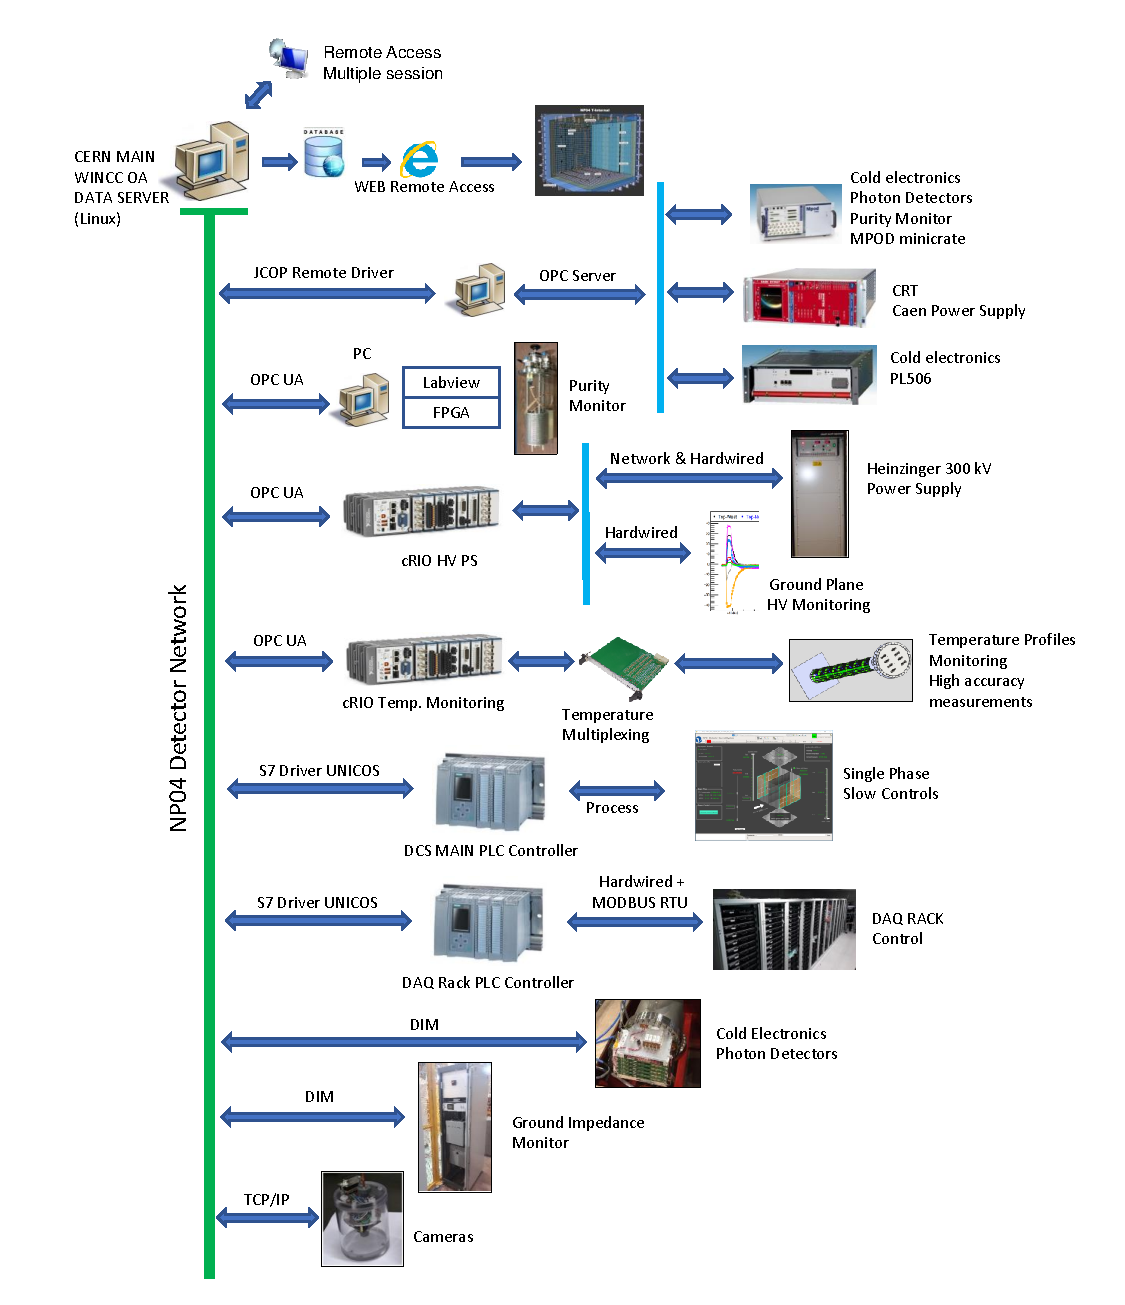
\includegraphics[height=0.9\textheight,width=0.95\textwidth,keepaspectratio]{NP04-DCS_arch_vert}
\end{dunefigure}

The \dword{pdsp} detector control system (also known as NP04-DCS) met
all requirements for operation in September, 2018, as
described in \cite{pdspdcs_proc}.  Those requirements are
nearly identical to those for \dword{fd} other than
total channel count. Of particular note, the NP04-DCS unified a heterogenous set of devices and data sources
through multiple protocols into a
single control system, as illustrated in
Fig.\ \ref{fig:cisc-NP04-DCS-topology}. In addition to what
the figure shows, data was also acquired from external cryogenic and beam
systems.  The topology and data flow of the system matches the general
shape shown in Fig.\ \ref{fig:gen-slow-controls-diagram}. In NP04-DCS,
the unified control system base is WinCC OA \cite{winccoa}, a
commercial toolkit used extensively at CERN, with device interfaces
supported using several standardized interface protocols.

As noted in the software and quantities sections above \fixme{Include the section numbers.} , the DUNE slow control
system will produce massive amounts of data, requiring a sizable database to store the value history and allow efficient data retrieval. Individually adjustable rates and thresholds for each channel are key in keeping this database manageable. The \dword{pdsp} operations provided not only a test of these features as implemented in the NP04 DCS, but also insight into reasonable values for these archiving parameters for each system.


%%%%%%%%
\section{Organization and Management}
\label{sec:cisc-slow-controls-org}

The organization of the CISC consortium is shown in
Figure~\ref{fig:gen-slow-cryo-org}. The CISC consortium board currently comprises institutional representatives from 19 institutes as shown in Table~\ref{tab:gen-slow-cryo-org}. \fixme{I counted 18 institutes, not 19. You might want to check that.} The consortium leader is the spokesperson for the consortium and responsible for the overall scientific program and managing the group. The technical leader of the consortium is responsible for managing the project for the group. Currently, the
consortium has five working groups:
\begin{description}
 \item[Cryogenics Systems] gas analyzers and liquid level
  monitors; \dword{cfd} simulations
 \item[Liquid Argon Instrumentation] purity monitors, thermometers, cameras and light emitting system, and instrumentation test facility; feedthroughs; \efield simulations; instrumentation precision studies; ProtoDUNE data analysis coordination and validation 
 \item [Slow Controls Base Software and Databases]  Base I/O software, alarms and archiving databases, and monitoring tools;
   variable naming conventions and slow controls quantities
 \item [Slow Controls Detector System Interfaces] Signal processing software and hardware interfaces (e.g., power supplies); firmware; rack hardware and infrastructure   
 \item [Slow Controls External Interfaces] Interfaces with external detector systems (e.g., cryogenics system, beam, facilities, \dword{daq}, near detector status)
\end{description}

\begin{dunefigure}[CISC consortium organization]{fig:gen-slow-cryo-org}
{CISC Consortium organizational chart}
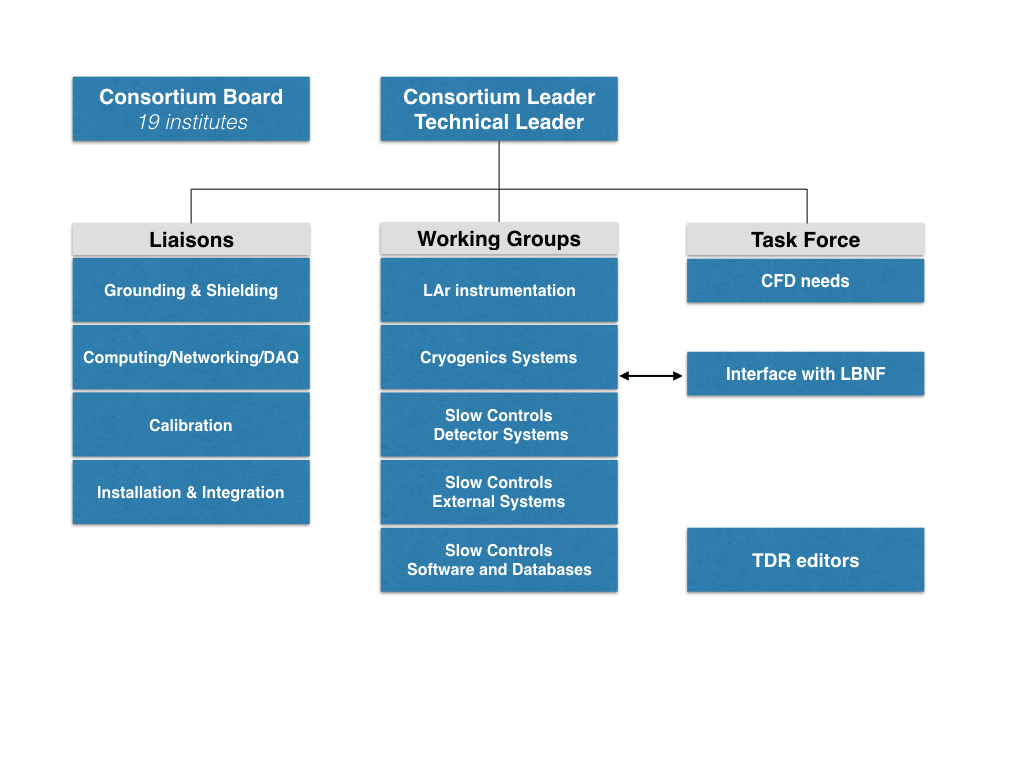
\includegraphics[width=0.7\textwidth]{cisc_org.png}
\end{dunefigure}

\begin{dunetable}
[CISC Consortium Institutions]
{p{0.43\textwidth}p{0.12\textwidth}p{0.22\textwidth}}
{tab:gen-slow-cryo-org}
{Current \dword{cisc} Consortium Board Members and their institutional affiliations}
Member Institute                         &  Country         &  Consortium Board Representative \\ \toprowrule
CIEMAT                                   &  Spain           &  Ines Gil Botella \\ \colhline
Instituto de Fisica Corpuscular (IFIC)          &  Spain           &  Anselmo Cervera \\ \colhline
University of Warwick                    &  UK  &  Gary Barker \\ \colhline
University College London (UCL)             &  UK  &  Mario Campanelli \\ \colhline
Argonne National Lab (ANL)                     &  USA             &  Jim Grudzinski  \\ \colhline
Brookhaven National Lab (BNL)                  &  USA             &  Jim Stewart \\ \colhline
University of California, Irvine (UCI)        &  USA             &  Jianming Bian \\ \colhline
Drexel University                        &  USA             &  Charles Lane \\ \colhline
Fermi National Accelerator Lab (FNAL)           &  USA             &  Alan Hahn \\ \colhline
University of Hawaii                     &  USA             &  Jelena Maricic \\ \colhline
University of Houston                    &  USA             &  Andrew Renshaw \\ \colhline
Idaho State University (ISU)                   &  USA             &  Ed Tatar \\ \colhline
Kansas State University (KSU)                  &  USA             &  Glenn Horton-Smith \\ \colhline
University of Minnesota, Duluth (UMD)         &  USA             &  Alec Habig \\ \colhline
Notre Dame University                    &  USA             &  John LoSecco \\ \colhline
South Dakota State University (SDSU)           &  USA             &  Stephen Gent \\ \colhline
University of Tennessee at Knoxville (UTK)     &  USA             &  Sowjanya Gollapinni \\ \colhline
Virginia Tech (VT)                            &	USA	            &  Camillo Mariani \\
\end{dunetable}

Moreover, because the CISC consortium broadly interacts with other groups, liaisons have been named as shown in Figure~\ref{fig:gen-slow-cryo-org}. 
%\todo{names need to go away from the org chart figure --> \textbf{Anselmo will fix it.}}. 
A short-term task force was recently formed to explore the need for cryogenic modeling for the consortium. A work plan for \dword{cfd} simulations for both ProtoDUNE and \dword{fd} was developed based on input from the task force. The \dword{tdr} editors are responsible for the overall editing and delivery of the \dword{tdr} document. Currently, members from new institutes are added to the consortium based on consensus from the consortium board members following an expression of interest petition from the new institute.

\subsection{Institutional Responsibilities}

The slow controls and cryogenic instrumentation will be a joint effort for single and dual phase. A single slow controls system will be implemented to serve both \dword{dp} and \dword{sp} detectors.

Design and installation of cryogenic systems (gas analyzers, liquid level monitoring) will be coordinated with \dword{lbnf}, with the consortium providing resources and effort, and expertise provided by \dword{lbnf}. ProtoDUNE designs for liquid argon instrumentation (purity monitors, thermometers, cameras, test facility) will be the basis for \dword{fd} designs. Design validation, testing, calibration, and performance will be evaluated through ProtoDUNE data.

Following the conceptual funding model envisioned for the consortium, various responsibilities have been distributed across institutions within the consortium. At this stage of the project, these should be considered as ``aspirational'' responsibilities until firm funding decisions are made. Table~\ref{tab:cisc-inst-resp} shows the current institutional responsibilities for primary \dword{cisc} sub-systems. Only lead institutes are listed in the table for a given effort. For physics and simulations studies, and validation efforts with ProtoDUNE, number of institutes are involved. A detailed list of tasks and institutional responsibilities are presented in \dword{dune} DocDB 5609.

\begin{dunetable}
[Institutional Responsibilities in the \dword{cisc} consortium ]
{p{0.4\textwidth}p{0.45\textwidth}}
{tab:cisc-inst-resp}
{Institutional Responsibilities in the \dword{cisc} consortium}
CISC Sub-system     &  Institutional Responsibility \\ \toprowrule
Purity Monitors          &  UCI, Houston \\ \colhline
Static T-Gradient Monitors     &  IFIC \\ \colhline
Dynamic T-Gradient Monitors & Hawaii \\ \colhline
Individual Sensors & IFIC \\ \colhline
Readout System for Thermometers & IFIC, Hawaii, CIEMAT \\ \colhline
Cold Cameras & KSU, BNL \\ \colhline
Warm Cameras & KSU, BNL \\ \colhline
Light-emitting System (for cameras) & Drexel \\ \colhline
Gas Analyzers & FNAL, \dword{lbnf} \\ \colhline
Liquid Level Monitors & \dword{lbnf}, Notre Dame \\ \colhline
Instrumentation Test Facility & FNAL, ANL \\ \colhline
\dword{cfd} Simulations & SDSU, ANL \\ \colhline
Other Simulation \& Validation Studies & Number of Institutes \\ \colhline
Slow Controls Hardware & UMD, UTK, Drexel\\ \colhline
Slow Controls Infrastructure & UMD, UTK\\ \colhline
Slow Controls Base Software & KSU, UTK, Drexel, Warwick, UCL, ANL, IFIC\\ \colhline 
Slow Controls Signal Processing & Number of institutes \\
\end{dunetable}

\subsection{Cost and Labor}

Table \ref{tab:cisc-cost} shows the current cost estimates for the \dword{cisc} subsystems. It also shows the quantity associated with each subsystem and a brief description of what is included in the cost estimate. The cost estimates only include materials and supplies (M\&S) and packing and shipping, but not labor and travel costs. Labor costs depend on personnel category (e.g., faculty, student, technician, post-doc, engineer) and vary by region and institution, so costs are quantified using labor hours needed to fulfill a given task. Table~\ref{tab:cisc-labor} provides estimates of labor hours for each subsystem, for a total of 95,010 labor hours for all \dword{cisc} tasks. 

\begin{dunetable}
[CISC Cost]
{p{0.3\textwidth}p{0.08\textwidth}p{0.1\textwidth}p{0.45\textwidth}}
{tab:cisc-cost}
{Cost estimates of the different CISC subsystems. All cost estimates include pacing and shipping costs.}
System                         & Quantity & Cost & Description  \\ \toprowrule
Purity monitors                & 10 & \$309,400 & Includes material cost, PC, flanges, mounting structure  \\ \colhline
Static T-gradient monitors     & 6 & \$88,340 & Includes cables, sensors and connectors, support structure, flanges \\ \colhline
Precision individual temperature sensors & 130 & \$51,512 & Includes cables, sensors and connectors, support structure, flanges \\ \colhline
Standard individual temperature sensors & 35 & \$12,615 & Includes cables, sensors and connectors, support structure, flanges \\ \colhline
Dynamic T-gradient monitors    & 2 & \$108,060 & Includes cables, sensors, motor drive, flanges, sensor holders \\ \colhline
Warm cameras                   & 3 & \$294,775 & Includes material cost, computer, argon purge \& pressurization system, prototyping \& testing  \\ \colhline
Cold cameras                   & 12 & \$38,300  & Includes material cost, computer, minor jigs \& test boards \\ \colhline
Light system                   & 15 & \$4,900 & Cost of illuminator and light driver module    \\ \colhline
Gas analyzers                  & 1 & \$222,360 & Cost of gas analyzers and piping \& routing panel  \\ \colhline
Capacitive level meters        & 4 & \$19,018  & Cost of level meters and flanges   \\ \colhline
Cryogenics test facility       & 1 & \$62,000  & Material cost includes liquid argon costs for years 1 to 5 and minor fixture costs  \\ \colhline
Slow controls hardware         & - & \$78,970  & Cost of 6 servers, 0.5 rack, 126 rack monitoring boxes, and cables   \\ \colhline
Slow controls software         & - & \$1,500 & Includes cost of a laptop    \\ \colhline
\textbf{Total Cost}          &       & \textbf{\$1,291,750}& \\
\end{dunetable}

\begin{dunetable}
[CISC labor]
{p{0.25\textwidth}p{0.15\textwidth}p{0.1\textwidth}p{0.08\textwidth}p{0.08\textwidth}p{0.1\textwidth}p{0.08\textwidth}}
{tab:cisc-labor}
{Estimate of labor hours for each category of personnel for different CISC subsystems. For slow controls software, the 884 technician hours comprises 442 hours from information technology professionals and 442 hours from scientific computing professionals.}
System  & Faculty/Scientist & Post-doc & Student & Engineer & Technician  &  \textbf{Total}\\ \toprowrule
& (hours) & (hours)& (hours)& (hours)& (hours)& (hours)\\ \toprowrule
Purity monitors & 5304& 5304& 5304& -& 1326 & \textbf{17238} \\ \colhline
Static T-gradient monitors & 3536& 1768& 2652&  442& 884& \textbf{9282} \\ \colhline
Individual temperature sensors & 3536& 1768& 2652&  442& 884& \textbf{9282} \\ \colhline
Dynamic T-gradient monitors & 3536& 3536& 3536&  354& 884& \textbf{11846} \\ \colhline
Warm cameras & 1768& 1768& 1768&  442& 737 & \textbf{6483}\\ \colhline
Cold cameras & 884& 1768& 1768& 100& 50& \textbf{4570}\\ \colhline
Light system & 884& - & 442 & - &20 & \textbf{1346}\\ \colhline
Gas analyzers & - & - & - &  320 & 480& \textbf{800}\\ \colhline
Level meters & - & - & - & 56 & - & \textbf{56}\\ \colhline
Cryogenic test facility & 1768& 2400& 2400& 180& 525& \textbf{7273}\\ \colhline
Slow controls hardware & 884 & 589& 884& 295 & 147& \textbf{2799}\\ \colhline
Slow controls software & 1768& 11492& - & 221 & 884& \textbf{14365}\\ \colhline
Physics \& simulation & 1768& 1768& 5604&  530 & - & \textbf{9670}\\ \colhline
\textbf{Total}  & \textbf{25636} & \textbf{32161}& \textbf{27010}& \textbf{3382}& \textbf{6821} & \textbf{95010}\\
\end{dunetable}

\subsection{Schedule}

%\fixme{SG: schedule table updated and new text added. Ready for review.}

Table \ref{tab:fdgen-slow-cryo-schedule} shows key construction milestones for the \dword{cisc} consortium leading to commissioning the first \dword{fd} module. \dword{cisc} construction milestones align with the overall construction milestones of the first \dword{fd} module (highlighted in bold in the table). The prototyping and testing of the final designs of \dword{cisc} systems is expected to be finished by 2020. The procurement and assembly of production units should start in 2021; integration tests largely done in 2022 \fixme{Will be performed in 2022 or will be finished in 2022?} . Installing instrumentation devices will start in December 2022 following the beneficial occupancy of the cryostat. Installing gas analyzers, level meters, individual temperature sensors, static T-gradient thermometers, and support structure for all instrumentation devices will finished before installing \dword{tpc}, but installing dynamic T-gradient thermometers, purity monitors, and cameras will occur afterward. \dword{cisc} will work closely with \dword{lbnf} to coordinate installation of the cryogenic systems and instrumentation devices. For slow controls, the goal is to have the full slow controls system commissioned and integrated into remote operations at least three months before the detector is ready for operations in 2025.  

%SG: I replaced the table with a different version of the table. Listing schedule WBS numbers is not needed and also it will be important to include the key milestones for the international schedule so it is easy to see that our plans align with that schedule.
\begin{comment}
\begin{dunetable}
[Key CISC Milestones leading to ...]
{p{0.05\linewidth}p{0.7\linewidth}p{0.05\linewidth}p{0.05\linewidth}}
{tab:fdgen-slow-cryo-schedule}
{Key CISC Milestones leading to ...}   
WBS     & Milestone                                                                                    & Start & Finish  \\ \toprowrule
2.1     & Cryogenic Instrumentation Local Test Facility ready                                          & 12/19 & 05/20   \\ \colhline
2.2     & Production of first full system prototypes of all CISC hardware devices                      & 11/19 & 06/20   \\ \colhline
2.3     & Test instrumentation device prototypes at the local test facility                            & 06/20 & 10/20   \\ \colhline
2.4     & Detector 1 (\dword{sp})                                                                    & 11/20 & 07/25   \\ \colhline
2.4.1   & Procurement of CISC hardware                                                                 & 11/20 & 03/21   \\ \colhline
2.4.2   & Assembly \& Production of CISC hardware                                                      & 03/21 & 02/22   \\ \colhline
2.4.3   & Local testing of CISC production hardware                                                    & 10/21 & 03/22   \\ \colhline
2.4.4   & Begin integrating/testing instrumentation devices in the cold box at the SURF ITF            & 04/22 & 11/22   \\ \colhline
2.4.5   & Begin integrating/testing Slow controls hardware/software at ITF (as part of the DAQ)        & 02/22 & 07/22   \\ \colhline
2.4.6   & Procure Gas Analyzers and Level meters                                                       & 03/22 & 06/22   \\ \colhline
%SG: Cryogenic piping no longer part of CISC, so removed these from schedule
%2.4.7   & Finish construction of Cryogenic Internal Piping                                             & 03/22 & 09/22   \\ \colhline
%2.4.8   & Installation of Cryogenic Internal Piping                                                    & 12/22 & 03/23   \\ \colhline
2.4.9   & Installation of Gas Analyzers                                                                & 12/22 & 03/23   \\ \colhline 
2.4.10  & Installation of support structure for all instrumentation devices                            & 03/23 & 04/23   \\ \colhline
2.4.11  & Installation of individual sensors, Static T-gradient thermometers and level meters          & 04/23 & 05/23   \\ \colhline
2.4.12  & All Slow Controls hardware, infrastructure \& networking installed                           & 08/23 & 02/24   \\ \colhline
2.4.13  & Slow Controls software for I/O, alarms, archiving, displays installed on production systems   & 02/24 & 05/24   \\ \colhline
2.4.14  & Install Dynamic T-gradient monitors, Cameras, Purity monitors after TPC installation         & 06/24 & 07/24   \\ \colhline
2.4.15  & Install all feedthroughs for instrumentation devices                                         & 07/24 & 07/24   \\ \colhline
2.4.16  & Install Slow Control Expert interfaces for all systems in time for testing                   & 05/24 & 09/24   \\ \colhline
2.4.17  & Full Slow controls systems commissioned and integrated into remote operations                & 04/25 & 07/25   \\ 
\end{dunetable}  
\end{comment}
                           
\begin{dunetable}
[Key \dword{cisc} construction milestones leading to the commissioning of the first \dword{fd} module.]
{p{0.7\linewidth}p{0.05\linewidth}p{0.05\linewidth}}
{tab:fdgen-slow-cryo-schedule}
{Key \dword{cisc} construction schedule milestones leading to commissioning the first \dword{fd} module.}   
Milestone  & Start & Finish  \\ \toprowrule
Cryogenic instrumentation local test facility ready                                          & 12/19 & 05/20   \\ \colhline
Production of first full system prototypes of all CISC hardware devices                      & 11/19 & 06/20   \\ \colhline
Test instrumentation device prototypes at the local test facility                            & 06/20 & 10/20   \\ \colhline
Procurement of CISC hardware                                                                 & 11/20 & 03/21   \\ \colhline
Assembly \& production of CISC hardware                                                      & 03/21 & 02/22   \\ \colhline
Local testing of CISC production hardware                                                    & 10/21 & 03/22   \\ \colhline
\textbf{Begin integrating and testing Detector\#1 components at ITF} & 02/22 & 02/22 \\ \colhline
Begin integrating/testing instrumentation devices in the cold box at the SURF ITF            & 04/22 & 11/22   \\ \colhline
Begin integrating/testing slow controls hardware/software at ITF (as part of DAQ)        & 02/22 & 07/22   \\ \colhline
Procure gas analyzers and level meters                                                       & 03/22 & 06/22   \\ \colhline
\textbf{Beneficial occupancy of cryostat\#1} & 12/22 & 12/22 \\ \colhline
Installation of gas analyzers                                                                & 12/22 & 03/23   \\ \colhline 
Installation of support structure for all instrumentation devices                            & 03/23 & 04/23   \\ \colhline
Installation of individual sensors, static T-gradient thermometers, and level meters          & 04/23 & 05/23   \\ \colhline
\textbf{Cryostat\#1 ready for TPC installation} & 05/23 & 05/23 \\ \colhline
All slow controls hardware, infrastructure, \& networking installed                           & 08/23 & 02/24   \\ \colhline
Slow controls software for I/O, alarms, archiving, displays installed on production systems   & 02/24 & 05/24   \\ \colhline
\textbf{Begin closing Cryostat\#1} & 05/24 & 05/24 \\ \colhline
Install dynamic T-gradient monitors, cameras, purity monitors after installing TPC          & 06/24 & 07/24   \\ \colhline
Install all feedthroughs for instrumentation devices                                         & 07/24 & 07/24   \\ \colhline
Install slow control expert interfaces for all systems in time for testing                   & 05/24 & 09/24   \\ \colhline
\textbf{Cryostat\#1 ready for filling} & 10/24 & 10/24 \\ \colhline
Full slow controls systems commissioned and integrated into remote operations                & 04/25 & 07/25   \\ \colhline
\textbf{Detector\#1 ready for operations} & 10/25 & 10/25   \\
\end{dunetable}                      

\subsection{Risks}
%\fixme{SG: Table reformatted and updated. New text added. This is now ready for review.}
Tables~\ref{tab:fdgen-slow-cryo-risk1}, \ref{tab:fdgen-slow-cryo-risk2}, and \ref{tab:fdgen-slow-cryo-risk3} list the possible risks identified by the \dword{cisc} consortium along with corresponding mitigation strategies. The tables list 18 risks at low and medium level. A more detailed list of risks with additional descriptions can be found in \cite{bib:docdb7192}. The tables show all risks are medium or low level, mitigated with necessary steps and precautions. Risk\#1, where the \dword{pdsp}-based designs are inadequate for \dword{fd}, is important because this requires early validation from ProtoDUNE data so R\&D of alternate designs can be timely. With \dword{pdsp} data now available, the consortium is focused on validating instrumentation designs.

\begin{dunetable}
[CISC risks1]
{p{0.05\linewidth}p{0.4\linewidth}p{0.05\linewidth}p{0.4\linewidth}}
{tab:fdgen-slow-cryo-risk1}
{Possible risk scenarios for the \dword{cisc} consortium along with mitigation strategies. The level of risk is indicated by letters ``H'', ``M'', and ``L'' corresponding to high, medium and low level risks.}   
No. & Risk  & Risk Level & Mitigation Strategy  \\ \toprowrule
1 & The baseline design (extrapolated from ProtoDUNEs) for instrumentation devices is not adequate for the \dword{fd}. & M & This should be detected early on such that R\&D on alternative designs can proceed on a reasonable time scale. \\ \colhline
%%%%SG: include the below one for DP chapter
%2 & Lack of involvement/expertise and insufficient input from past experience from \dword{dp} & M & Seek help from management to ensure DP expertise and involvement is provided at the needed level to the Consortium. Information transfer from DP side is critical when direct involvement and contribution is not possible. \\ \colhline
2 & Potential swinging of long instrumentation devices (T-gradient monitors or purity monitors) due to e.g. mis-alignment at the top. & L & Add additional intermediate anchoring points (as needed) to prevent swinging. 
\\ \colhline
3 & High \efield near instrumentation devices could lead to dielectric breakdowns. & L & Instrumentation systems will be placed as far away as possible from the cathode, \dword{fc} and other \dword{tpc} components where the fields are expected to be low and additional shielding is not required. For \dword{dp}, shielding is anticipated for devices as it is impossible to find low-field regions.
\\ \colhline
4 & Light pollution from purity monitors and camera light system could potentially interfere with physics measurements and damage the \dword{pds}. & L &
Purity monitors and camera systems could be run at definite times and a signal sent to the detector to veto any signals during their operation. For purity monitors, software for light source triggering mechanism will be developed to prevent the flash lamp from operation during photon detector's triggering windows. 
\\ \colhline
5 & Temperature sensors can induce noise in cold electronics. & M & If noise is discovered before cryostat filling, check all connections, mainly the ones to ground. If noise is discovered after cryostat filling, address the problem at the readout level (e.g. noise filters). If problem persists connect offending sensors to ground using dummy connectors with all pins grounded. 
\\ \colhline
6 & Disagreement between lab and in-situ calibrations for dynamic T-gradient monitor. & M & Understand which of the two calibrations is wrong or has more limitations; improve both methods especially the laboratory one since this is the only method for sensors behind APAs, and top and bottom of the detector. 
\\ \colhline
7 & Purity monitor electronics induce noise in cold electronics. & M & Develop software for light source triggering mechanism to prevent the purity monitor flash lamp from operation during photon detector data taking. Use Faraday cage to ground the light source. 
\\
\end{dunetable}    

\begin{dunetable}
[CISC risks2]
{p{0.05\linewidth}p{0.4\linewidth}p{0.05\linewidth}p{0.4\linewidth}}
{tab:fdgen-slow-cryo-risk2}
{Possible risk scenarios for the \dword{cisc} consortium along with mitigation strategies. The level of risk is indicated by letters ``H'', ``M'', and ``L'' corresponding to high, medium and low level risks. The numbering for listed risks continued from the previous table.}   
No. & Risk  & Risk Level & Mitigation Strategy  \\ \toprowrule
8 & Discrepancies between measured temperature map and \dword{cfd} simulations in \dword{pdsp} can have potential impact on physics as physics relies on simulations to extract various calibration quantities. & L
& Improve simulations with more precise  inputs from real measurements (e.g. liquid argon flows, temperature of incoming \dword{lar}, temperature of gaseous argon in the ullage); use a fraction of temperature sensors to predict temperatures in other parts of the cryostat.  
\\ \colhline
9 & Difficulty in correlating data from purity monitors and thermometers can impact understanding of the behavior of cryogenics system. & L & Understand what aspect (design, drift physics etc.) is causing the discrepancy and if any modifications in the design are needed. One option would be to instrument the purity monitors with temperature sensors such that purity and temperature are measured in the same location.
\\ \colhline
%****SG: Should we include the cold camera risk? as good progress is being made at ProtoDUNE. It just needs more R&D, right? I am inclined to drop this.******%
10 & During R\&D phase the consortium is not able to build a working prototype for cold cameras that meets all the requirements \& safety. This risk originates from the fact that cold cameras are not operational after a period of time in \dword{lar} or show low performance (e.g. delays, bad resolution) & M & Further pursue R\&D: e.g. improve thermal insulation and heaters, use alternative camera models. If problems persist use cameras at the ullage with the appropriate field of view and lighting  such that elements inside \dword{lar} can be inspected. Also, understand the importance of cold cameras for \dword{hv} diagnosis as not having them may put \dword{hv} at risk. \\ \colhline
11 & Cameras can induce \dword{hv} discharge. & M & Electric field in the camera housing and related anchoring systems must be studied carefully such that proper shielding is employed. 
\\ \colhline
12 & \dword{hv} discharge can damage cameras as some of them will be located near \dword{hv} devices. With proper shielding included, this is very unlikely but there is some risk. & M & The most important cameras should have enough redundancy such that the loss of one camera does not compromise the overall performance.
\\ \colhline
13 & Cameras have insufficient light to see. The attenuation of light in \dword{lar} could prevent cameras from seeing objects in the deep regions of the cryostat. & M & Cameras will have to be tested during the R\&D phase under conditions of illumination expected in the actual detector. The cryogenics instrumentation test facility should have sufficient depth for testing this risk scenario. \\ \colhline
14 & Cameras may induce noise in cold electronics. & M & Work with the grounding and shielding group to ensure proper grounding. \\ 
\end{dunetable}  

\begin{dunetable}
[CISC risks3]
{p{0.05\linewidth}p{0.4\linewidth}p{0.05\linewidth}p{0.4\linewidth}}
{tab:fdgen-slow-cryo-risk3}
{Possible risk scenarios for the \dword{cisc} consortium along with mitigation strategies. The level of risk is indicated by letters ``H'', ``M'', and ``L'' corresponding to high, medium and low level risks. The numbering for listed risks are continued from the previous table.}   
No. & Risk  & Risk Level & Mitigation Strategy  \\ \toprowrule
15 & Light attenuation in long optic fibers of the purity monitors can result in insufficient intensity to produce enough drift elections for the purity measurement. & M & Test the maximum length of fiber that can be used and optimize the depth of the bottom purity monitor and the number of fibers to be run accordingly. 
\\ \colhline
16 & Longevity of Purity Monitors. The current design could fail if operated in impure liquid or gaseous argon because of the degradation of photocathode for a long time. & M & Design software deadlock to prevent monitors from running long time when low purity is detected. The degradation can be recovered in many ways: 1. by running high frequency/intensity xenon flashes for a few days after purity is recovered, 2. by using RTDs to heat cathode, as the primary contamination on a degraded cathode surface is likely to be ice or water compound from the impurity. 
%We will supply each PrM with more fibers thus provide higher intensity light coming from the fibers  In case that the contamination that causes degradation can not be removed completely.  This would also illuminate more surface area of the photocathode and may result in more life to the photocathode as well. 
The best way to mitigate the degradation is to have monitors inline with the cryogenics purification system and have them in valves so they can be maintained over time.  This would ensure that the purity of the \dword{lar} is always being monitored, even if not directly in the cryostat. 
\\ \colhline
% 18
% &
% Additional level meters required
% &
% The baseline design consists of two differential pressure level meters at the two detector far ends. Those are needed by the cryogenics system. Additional level meters could be needed by the detector, the requirements of which need to be understood.
% &
% L
% &
% Add additional level meters based on temperature and/or capacitive measurements, as done for ProtoDUNE-SP
% \\ \toprowrule
%****SG: remove this, this is an overkill at this point as I can't imagine not accommodating testing of alternate devices in CITF.****
%19 & The baseline design of the Cryogenics Instrumentation Test Facility (CITF) is not suitable for some of the alternative designs mentioned in risk 1 in Table~\ref{tab:fdgen-slow-cryo-risk1}. & L & The constraints of the CIFT should be taken into account when designing new prototypes, so that such that those new designs can be easily accommodated in the CIFT.   \\ \colhline
17 & Longevity: Gas analyzers and level meters may fail. These are commercial devices with typical warranties around one year from date of purchase. & L &
To mitigate this, make provisions for future replacement in case of failure or loss of sensitivity. 
\\ \colhline
% 21
% &
% Cryogenic Internal Piping
% &
% Design of the internal cryogenics is more complex than expected and costs more than anticipated.
% &
% L
% &
% Expand the conceptual design done so far and advance it further before outsourcing it.
% \\ \toprowrule
18 & Problems in interfacing  hardware devices (e.g. power supplies) with slow controls. & M & The choice of power supplies and other hardware devices that need control/monitoring should be made in consultation with slow control experts to ensure the hardware choices allow for robust control/monitoring at the precision needed. \\
\end{dunetable}

\begin{comment}
\begin{table}
\tiny
\begin{tabular}{p{0.01\textwidth}p{0.15\textwidth}p{0.3\textwidth}p{0.02\textwidth}p{0.35\textwidth}}
%\begin{dunetable}
%[Risks]
%{p{0.03\textwidth}p{0.2\textwidth}p{0.3\textwidth}p{0.04\textwidth}p{0.3\textwidth}}
%{tab:fdgen-cisc-risk}
%{Risks}   
ID	& Title	& Explanation &	Risk Level	& Mitigation \\ \toprowrule
1	& 
The baseline design (extrapolated from ProtoDUNEs) for any of the instrumentation devices is not adequate for DUNE far detectors	
&
The design of most instrumentation devices is based on extrapolation from ProtoDUNEs (mainly SP) design. Unforeseen problems could be discovered in terms of design and performance during installation, commissioning and data analysis in ProtoDUNEs
&
M
&
This potential problem should be detected as soon as possible (soon after ProtoDUNE data taking starts) such that R\&D on alternative designs can proceed on a reasonable time scale. The concept of those alternative designs should exist by the time of the TDR
\\ \toprowrule
2
&
Lack of involvement/expertise and insufficient input from past experience on instrumentation devices for dual-phase technology
&
DUNE DP far detector will need additional considerations (different \efield structure, more precise LAr level measurements, etc), which are not necessary for the SP detector. Will need involvement and input from current DP experts to arrive at a successful design.	
&
M
&
Seek help from Technical Coordinator and Spokespeople to ensure DP expertise and involvement is provided at the needed level to the Consortium. Information transfer from DP side is critical when direct involvement and contribution is not possible. \\ \toprowrule
3
&
Potential swinging of long instrumentation devices (T-gradient monitors or PrM system) due to e.g. mis-alignment at the top	
&
In principle those systems will hang from the top of the cryostat (either from their flange or from bolts on the corners) and could potentially be anchored at the bottom near the corners for devices that go across the full height of the detector.
&
L
&
Add additional intermediate anchoring points (as needed) to prevent swinging by welding the appropriate element to the cryostat membrane. This option must be discussed with the cryostat management as soon as possible.
\\ \toprowrule
4
&
High electric fields near instrumentation devices (purity monitors, temperature gradients, cameras, etc)
&
The instrumentation systems need to be mounted within the cryostat such that it is far enough away from the FC such as not to cause very high electric fields which could then lead to dielectric breakdown across the LAr.
&
L
&
Instrumentation systems will be placed as far from the cathode, field cage and other TPC components as possible, most likely near the corner of the cryostat, or above/below ground planes, where the fields should be low enough for the system to not require additional shielding from high fields. In the DP FD module, since it is impossible to find low field regions, shielding is anticipated for instrumentation devices to prevent high fields. 
\\ \toprowrule
5
&
Light pollution from purity monitors and camera light emitting system	
&
The light source for the Purity Monitor system or the light emitting system for cameras will produce a lot of UV light in the detector which could potentially interfere with physics measurements and damage the Photon Detector System.  	
&
L
&
PrM and camera systems could be run at definite times and a signal sent to the detector to Veto any signals during PrM or camera system measurements.  For PrMs, software for light source triggering mechanism will be developed to prevent the PrM flash lamp from flashing during photon detector's triggering windows. One can also consider using this light signal to calibrate the photon detector system at the same time.
\\ \toprowrule
6
&
Temperature sensors can induce noise in cold electronics
&
Each temperature sensor is readout with a cable with four wires, which are shielded against EM noise. The shield should be connected to ground. If this connection is not properly done EM noise from outside the cryostat can be introduced through the cables
&
M
&
If noise is discovered before filling the cryostat check all connections, mainly the ones to ground. If noise is discovered after cryostat filling try to solve the problem at the readout level (e.g. noise filters). If problem persists connect offending sensors to ground using dummy connectors with all pins grounded  
\\ \toprowrule
7
&
Disagreement between lab and in-situ calibrations for ProtoDUNE-SP dynamic T-gradient monitor
&
Temperature sensors in the dynamic T-gradient monitor are calibrated using two methods: lab calibration to 0.002 K (as in the static T-gradient monitor)  and in-situ cross-calibration moving the system vertically.
&
M
&
Try to understand which of the two calibrations is wrong or has more limitations. Try to improve both methods, specially the laboratory calibration since this is the only one possible for sensors behind APAs, and top/bottom of the detector. 
\\ \toprowrule
8
&
Discrepancies between measured temperature map and CFD simulations in ProtoDUNE-SP
&
Significant discrepancies between real data and simulations. Can have potential impact on physics as physics relies on simulations to extract various calibration quantities.
&
L
&
Improve simulations with more precise  inputs from real measurements: liquid argon flows, temperature of incoming LAr and temperature of gas argon in the ullage, etc. Use a fraction of T-sensors to predict temperatures in others.  
\\ \toprowrule
9
&
Experience with ProtoDUNE shows that it is difficult to correlate data from PrMs and Thermometers
&
Liquid argon purity as measured by the purity monitors, and vertical temperature gradients should be correlated and this correlation is important to understand the behavior of cryogenics system.
&
L
&
Understand what aspect (design, drift physics etc.) is causing the discrepancy and if any modifications in the design are needed to arrive at better agreement. One option could be to instrument the purity monitors with temperature sensors such that purity and temperature are measured in the same location
\\ \toprowrule
10
&
During R\&D phase the CISC consortium is not able to build a working prototype for cold cameras that meet all the requirements \& safety
&
Cold cameras are not able to work for longtime or show low performance (e.g. delays, bad resolution)
&
M
&
Further pursue R\&D: Improve thermal insulation and heaters, use alternative camera models, etc. If problems persist use cameras at the ullage with the appropriate field of view and lighting  such that elements inside LAr can be inspected. Also, better understand the importance of the cold cameras for HV diagnosis and if not having them will put HV at risk.
\\ \toprowrule
11
&
HV discharge caused by the cameras
&
Cameras can induce HV discharge. Unlike other instrumentation devices which will mostly be fixed at one location, cameras will be deployed as needed (within safety limits) to inspect or monitor HV activity.
&
M
&
Electric field in the camera housing and related anchoring systems must be studied carefully such that the proper shielding is used. Eventually those could be tested in a HV testing facility
\\ \toprowrule
12
&
HV discharge destroying the cameras
&
Cameras are delicate devices as some of them will be located near HV devices. Provided the proper shielding it is very unlikely that cameras are destroyed by discharges, but there is some risk
&
M
&
The most important cameras should have enough redundancy such that the lost of one camera does not compromise the overall performance 
\\ \toprowrule
13
&
Cameras have Insufficient light to see
&
Specially important will be the attenuation of light inside LAr, which could prevent cameras from seen things in deep areas of the cryostat.
&
M
&
Cameras will have to be tested during the R\&D phase under conditions of illumination similar to the ones of the actual detector. The cryogenics instrumentation test facility should have sufficient depth for testing the ability of seen deep objects.
\\ \toprowrule
14
&
Cameras may induce noise in cold electronics
&
Noise from the consumer grade electronics used by the camera systems and how it interacts with the surrounding detector elements.
&
M
&
Need to work with the camera team and grounding and shielding group to further understand this concern and develop possible mitigation strategies.
\\ \toprowrule
15
&
Purity monitors electronics introduces noise in cold electronics
&
The only electric noise from PrM is caused by the current surge in the  discharging process of the  main capacitor of the xenon light source when producing a flash
&
M
&
Develop software for light source triggering mechanism to prevent the PrM flash lamp from flashing during photon detector data taking. Use Faraday cage to ground the light source. 
\\ \toprowrule
16
&
Light attenuation in long optic fibers for Purity Monitors
&
For the PrMons at the bottom of the cryostat, if the fibers are too long the attenuation of the light inside them could be too much and not provide enough intensity to give enough drift elections to make the measurement.
&
M
&
Test the maximum length of fiber that can be used. The depth of the bottom PrMons would then be optimized based on this measurement and the number of fibers that is reasonable to run to the bottom PrMons.
\\ \toprowrule
17
&
Longevity of Purity Monitors
&
The current design of these devices could fail if operated in impure liquid or gas argon because of the degradation of photocathode for a long time. A significant photocathode degradation was observed during LAPD running when the cryo-pump failed for a few days. In principle, since Purity Monitors are most useful during commissioning, this may not be a major issue but since cosmic muons will be sparse in the FD, with no purity monitors, we may be at a risk for monitoring purity especially after recovering from cryogenic issues, power outages etc. when one cannot use tracks to make the purity measurement.
&
M
&
This problem can be solved by design software deadlock to prevent PrMs from running a long time when detecting a very low purity. The degradation can be recovered by running high frequency and intensity xenon flashes for a few days after purity recovered. The degradation can also be recovered by using RTD to heat cathode, because the primary contamination on a degraded cathode surface is likely to be ice or water compound from the impurity. We will supply each PrM with more fibers thus provide higher intensity light coming from the fibers  In case that the contamination that causes degradation can not be removed completely.  This would also illuminate more surface area of the photocathode and may result in more life to the photocathode as well.  The best way to mitigate this degradation problem is to have the monitors which are inline with the cryogenics purification system and have them valves so they can be maintained over time.  This would ensure that the purity of the LAr is always being monitored, even if not directly in the cryostat. 
\\ \toprowrule
% 18
% &
% Additional level meters required
% &
% The baseline design consists of two differential pressure level meters at the two detector far ends. Those are needed by the cryogenics system. Additional level meters could be needed by the detector, the requirements of which need to be understood.
% &
% L
% &
% Add additional level meters based on temperature and/or capacitive measurements, as done for ProtoDUNE-SP
% \\ \toprowrule
19
&
The baseline design of the Cryogenics Instrumentation Test Facility (CITF) is not appropriate for some of the alternative designs mentioned in risk 1
&
The final design of some of the instrumentation devices could differ from those described in the TP/TDR. This could have implications in the CITF design.
&
L
&
The constraints of the CITF should be taken into account when designing new prototypes, so that such that those new designs can be easily accommodated in the CITF.   
\\ \toprowrule
20
&
Longevity: Gas analyzers and level meters may fail.
&
The active electronics parts of both Gas Analyzers and level transducers are external to the cryostat. These devices cannot be required to last 20 years--these are commercial devices purchased at some point in their product cycle. One must expect that at some stage, replacement devices may need to be purchased.  Typical warranties are ~1 year from date of purchase.
&
L
&
To mitigate this, make provisions for for future replacement in case of failure or loss of sensitivity. 
\\ \toprowrule
% 21
% &
% Cryogenic Internal Piping
% &
% Design of the internal cryogenics is more complex than expected and costs more than anticipated.
% &
% L
% &
% Expand the conceptual design done so far and advance it further before outsourcing it.
% \\ \toprowrule
22
&
Problems in interfacing  hardware devices (e.g. power supplies) with slow controls
&
Slow controls team could have problems to monitor/control some hardware devices which do not have the necessary services/options
&
M
The choice of HV/LV power supplies and other hardware devices that need control/monitoring should be done in consultation with slow control experts to ensure the hardware choice allows for robust control/monitoring at the precision needed. 
%\end{dunetable}
\end{tabular}
\end{table}
\end{comment}

\subsection{Synergistic Activity}
\label{sec:interfaces}

The \dword{cisc} consortium interfaces \fixme{Try interaction instead of interface. I have to state that I truly dislike using the word "interface" for communication between people. As far as I am concerned, "interface" should only apply to technology, where it has a technical, and meaningful, definition. The word "interaction" might be a better choice. I have also seen "synergystic activity," which is problematic in other ways but avoids the problem with definition.} with all other detector consortia, task forces (calibration),
working groups (physics, software/computing, beam instrumentation), and technical coordination. We also interact heavily with \dword{lbnf} (beam and cryogenics groups).  
Detailed descriptions of \dword{cisc} interfaces are maintained in \dword{dune} DocDB. A brief summary is provided in this section. Table~\ref{tab:fdgen-cisc-interfaces} lists the IDs of the different DocDB documents as well as their highlights. Descriptions of the synergystic activities that affect many systems are given below. 

Obviously, \dword{cisc} interacts with the detector consortia because \dword{cisc} will provide status monitoring of all important detector sub-systems along with controls for some components of the detector.
%full rack monitoring (rack fans, thermometers and rack protection system), interlock status bit monitoring (not the actual interlock mechanism) and monitoring and control for all power supplies (PS).
\dword{cisc} will also consult on selecting different power supplies to ensure monitoring and control can be established with preferred types of communication. 
Rack space distribution and interaction between slow controls and other modules from other consortia will be managed by TC in consultation with those consortia. 

If heaters/RTDs are needed on flanges, CISC will specify the heaters/RTDs and will provide the readout/control, while the responsibility for the actual hardware will be discussed with the different groups.  

Installing instrumentation devices will interfere with other devices and must be coordinated with the the appropriate consortia.  
On the software side, \dword{cisc} must define, in coordination with other consortia/groups, the quantities to be monitored/controlled by slow controls and the corresponding alarms,
archiving, and GUIs. 


\begin{dunetable}
[Interfaces]
{p{0.2\textwidth}p{0.08\textwidth}p{0.62\textwidth}}
{tab:fdgen-cisc-interfaces}
{Synergistic activity documents}   
Consortium, Task force or TC   & {\bf DocDB} & {\bf Summary} \\ \toprowrule
APA	                           & 6679  &

The APA consortium will review the design and locations of the static T-gradient monitors to ensure
no electrical interference with the APA and no possibility of coming in contact with the APA wire planes.
Location of cameras/lights (provided by CISC) for inspection of health of APA wires.
\\ \colhline

Photon Detection	           & 6730  & 

PrMs and light emitting system for cameras both emit light that might damage PDs.
Under consideration hardware interlocks that avoid turning on lights accidentally when PDs are on.
\\ \colhline

TPC Electronics	               & 6745  & \\ \colhline


HV Systems	                   & 6787  &

safety issues. \efield simulations to guaranty proper shielding (\dword{cisc} responsibility with HV guidance).
Avoid generation of bubbles any time the inspection camera is inside the cryostat, as it can lead to discharges when the HV is turned on. 

CISC must understand the location of cold cameras and lights for inspection of HV related devices, as well as the requirements of cold/warm cameras. 
Ground planes (GP) could be used as support for cold cameras and individual temperature sensors. 
\\ \colhline

DAQ	                           & 6790  &

Also described in section~\ref{sec:fd-daq-intfc-sc}. Description of \dword{cisc} data storage, 
allowing bi-directional communications between \dword{daq} and \dword{cisc}.
\\ \colhline
Calibration         	       & 7072  &

\dword{cisc}/CTF ports will be multi-purpose to enable deploying various devices (flange design and space share around ports must be agreed). 
Calibration ports could be used to extract cables from \dword{cisc} devices. 
%At the software level CISC will be responsible for calibration device monitoring (and control to the extent needed) and will 
%monitor the interlock bit status for Laser and radioactive sources. (NO NEED TO REPEAT THIS SINCE IS THE SAME FOR ALL DETECTOR CONSORTIA)
%Understand the location of Cold cameras & lights for inspection of CFT related devices, as well as the
%requirements of Cold/Warm cameras: resolution, field of view, light sensitivity, low light operation, frames per second, operation in triggered mode?  etc.
\\ \colhline
Physics	                       & 7099  &

Indirect interfaces through calibration. Tools to extract data from the slow controls database (see \dword{cisc}-SWC interface document)
are required in order to correlate high level quantities to low level or calibration data. A brief list of what CISC data is needed by Physics is given in DocDB. 
\\ \colhline

Software \& Computing	       & 7126  &

Assuming that the scope of software \& computing (SWC) group includes scientific computing support to project activities, there are substantial hardware and software
interfaces with that group 
\\ \colhline

Cryogenics                     &  -    &

As mentioned in Sec.~\ref{sec:fdgen-slow-cryo-purity-mon} purity monitors and gas analyzers will be essential
to mitigate the liquid argon contamination risk. The appropriate interlock mechanism to prevent the cryogenics system from irreversible contamination
must be designed and implemented. 
\\ \colhline


Beam                           &  -    &  

At least the status of this system will be monitored
\\ \colhline

TC Facility                    & 6991  & \\ \colhline
TC Installation     	       & 7018  & \\ \colhline
TC Integration Facility        & 7045  & \\ 
\end{dunetable}



%% \begin{dunetable}
%% [Interfaces]
%% {p{0.2\textwidth}p{0.06\textwidth}p{0.64\textwidth}}
%% {tab:fdgen-cisc-interfaces}
%% {Interface documents}   
%% Consortium/Task force              & DocDB & summary \\ \toprowrule
%% SP APA	                           & 6679  & \\ \colhline

%% SP Photon Detection	               & 6730  & \\ \colhline

%% SP TPC Electronics	               & 6745  & \\ \colhline

%% DP CRP	                           & 6760  & \\ \colhline

%% DP Photon Detection	               & 6781  & 

%% PrMs and light emitting system for cameras both emit light that might damage PDs.
%% May have to define the necessary hardware interlocks
%% that avoid turning on any other light source accidentally when PDs are on.
%% \\ \colhline

%% DP TPC Electronics 	               & 6784  & \\ \colhline

%% HV Systems	                       & 6787  &
%% \begin{itemize}
%% \item safety issues
%% \item \efield simulations to guaraty proper shielding is CISC responsibility with HV guidance. 
%% \item During the deployment of inspection cameras, generation of bubbles must be avoided when HV is on, as it can lead to discharges.
%% \end{itemize}
  
%% \\ \colhline

%% DAQ	                               & 6790  &

%% Also described in section~\ref{sec:fd-daq-intfc-sc}. 
%% CISC data will be stored both locally (in CISC database servers in the
%% CUC) and offline (the databases will be replicated back to Fermilab)
%% in a relational database indexed by timestamp.
%% This will allow bi-directional communications between DAQ and CISC by
%% reading or inserting data into the database as needed for non
%% time-critical information.  
%% \\ \colhline

%% TC Facility Interfaces             & 6991  & \\ \colhline
%% TC Installation Interfaces	       & 7018  & \\ \colhline
%% TC Integration Facility Interfaces & 7045  & \\ \colhline
%% Calibration Task Force	           & 7072  &
%% \begin{itemize}
%% \item CISC and CTF ports will be multi-purpose to enable deploying various devices,
%% \item both systems will need to interact in terms of flange design and sharing space around the ports. Also, CISC might use calibration ports to extract cables from CISC devices. 
%% \item At the software level CISC will be responsible for calibration device monitoring (and control to the extent needed) and will 
%% monitor the interlock bit status for Laser and radioactive sources. 
%% \end{itemize}
%% %Understand the location of Cold cameras & lights for inspection of CFT related devices, as well as the
%% %requirements of Cold/Warm cameras: resolution, field of view, light sensitivity, low light operation, frames per second, operation in triggered mode?  etc.
%% \\ \colhline

%% Physics	                           & 7099  &

%% indirec through the CFT devices. One specific need for physics will be to extract
%% instrumentation or slow controls data to correlate high level quantities to low level or calibration data.
%% This requires tools to extract data from the slow controls database (see CISC-SWC interface document \cite{bib:docdb7126}).
%% A brief list of what CISC data is needed by Physics is given in the CISC-Physics interface document \cite{bib:docdb7099}. 
%% \\ \colhline

%% Software \& Computing	           & 7126  &

%% Assuming that the scope of software \& computing (SWC) group includes scientific computing support to project activities, there are substancial interfaces with that group \cite{bib:docdb7126}. 
%% The hardware interfaces resposibility of the SWC include networking installation and maintenance,
%% maintenance of SC servers and any additional computing hardware needed by instrumentation devices.
%% CISC will provide the needed monitoring for power distribution units (PDUs). Regarding software interfaces the SWC group will provide:
%% i) SC database maintenance, ii) API for accessing the SC database offline,
%% iii) UPS packages, local installation and maintenace of software needed by CISC, and iv) SWC creating and maintaining computer accounts on production clusters. 
%% On the other direction CISC will provide the required monitoring/control of SWC quantities including alarms, archiving and GUIs when applicable. 
%% \\
%% \end{dunetable}



%Rack space distribution and interaction between slow controls (SC) modules and other modules (APAs, HV, PD, DAQ, etc)

%SC signals into main DAQ data stream and viceversa


%The location of cold cameras and lights for inspection of HV related devices,
%as well as the requirements of cold/warm cameras (see Sec.~\ref{sec:fdgen-slow-cryo-cameras}) have to be understood
%in cooperation with HV consortium.
%Special software may be needed to detect discharges using the camera system,
%which will be the responsibility of the HV consortium.
%Finally, ground planes will be used as support for temperature sensors. The integration of the two systems must be understood. 




%\fixme{Does this x-ref work?  The cut-n-paste below (commented out) from
%  the official interfaces document seems overkill.  Also, there are not
%  currently plans for a DAQ test stand at SURF.  The DAQ as a whole is
%  installed before APAs arrive, then the actual DAQ used to commission
%  the APAs as they go in.  If the there is a slow controls test facility
%  at SURF, the same software interfaces could be used as for the final
%  form, nothing new needs created.}


%DAQ status.  


%The interface with the facility: .... Building controls; Detector hall monitoring; ground impedance monitoring

%  Power distribution units monitoring; Computer hardware monitoring

%\fixme{specify external interface of Cryo Inst. Systems with systems outside the cryostat (with LBNF), detector Interface to LBNF design teams working on the design on cryogenic systems (including cryogenic piping), The switchyard for the gas analyzers ... }


%Interfaces with the Facility are: Location of instrumentation devices, anchoring points, cryostat ports and flanges,
%space needed above cryostat, cable routing, rack space above cryostat, Mezzanine and CUC (Central Utility Cavern), etc 


%\fixme{Describe interface with DAQ system, including Interface with
%  DAQ/Electronics groups for a slow controls test facility at SURF,
%  possibly as part of the DAQ test stand.}  







%%%%%%%%%%%%%%%%%%%%%%%%%%%%%%%%%%%
%\subsection{Interface with Environmental and Building Controls}
%\label{sec:fdgen-slow-cryo-slow-enviro}

%\fixme{describe interface with LBNF on environmental and building controls}

%Building Temperature, humidity and pressure will be monitored and integrated into the slow controls system. 



\subsection{Installation, Integration, and Commissioning}


\subsubsection{Purity Monitors}
\label{sec:fdgen-slow-cryo-instal-pm}

%\fixme{IIC Purity Monitors: too much repetition. It can be shortened. To be reviewed: [CP] slightly modified to avoid repetitions}

The purity monitor system will be built in moduls, so it is can be assembled outside the DUNE-FD cryostat  
%The assembly of the purity monitors themselves would occur outside of the cryostat and would include everything described in the previous section.  The installation of the purity monitor system can then be carried out 
with the fewest steps left to complete inside the cryostat.  The assembly itself should come into the cryostat with the three individual purity monitors mounted to support tubes, with no HV cables or optical fibers yet installed.  The support tube at the top and bottom of the assembly would then be mounted to the brackets inside the cryostat; the brackets could be attached to the cables trays and/or the detector support structure.  At much the same time, the front-end electronics and light source can be installed on the top of the cryostat, and the electronics and power supplies can be installed in the electronics rack.  

Integration would begin by running the HV cables and optical fibers to the purity monitors, through the top of the cryostat.  The HV cables would be attached to the HV feedthroughs with sufficient length to reach each purity monitor inside the cryostat.  
The cables would be run along cable trays through the port reserved for the purity monitor system. 
%inside the cryostat until they reach the purity monitor system, and would then be terminated through the support tube down to each of the purity monitors.  
Each purity monitor will have three HV cables that connect it to the feedthrough and then further along to the front-end electronics.  The optical fibers would then be run through the special optical fiber feedthrough, into the cryostat, and would be guided to the purity monitor system either using the cables trays or guide tubes, depending on which solution is adopted. 
%for running the optical fibers from the feedthrough to the purity monitor system, 
This should protect fibers from breaking accidentally as the rest of the detector and instrumentation installation continues.  The optical fibers would then be run inside the purity monitor support tube and to the appropriate purity monitor, terminating the fibers at the photocathode of each monitor while protecting them from breaking near the purity monitor system itself.

Integration would continue as the HV cables are connected through the feedthrough to the system front-end electronics; then optical fibers are connected to the light source.  The cables connecting the front-end electronics and the light source to the electronics rack would also be run and connected at this time.  This allows the system to be turned on and the software to begin testing the various components and connections.  Once all connections are confirmed successful, integration with the slow controls system would begin, first by establishing communication between the two systems and then transferring data between them to ensure successful exchange of important system parameters and measurements.  

Commissioning the purity monitor system would be official once the cryostat is purged and a gaseous argon atmosphere is present.  At this time, the HV for the purity monitors could be ramped up without fear of discharge through the air, and the light source turned on.  Although the drift electron lifetime in the gaseous argon would be very large and therefore not really measurable with the purity monitors themselves, the signal strength at both the cathode and anode would give a good indication of how well the light source generates drift electrons from the photocathode and that the electrons successfully drift to the anode by looking at the signal strength at the anode and comparing it to the cathode signal strength.

\subsubsection{Thermometers}
\label{sec:fdgen-slow-cryo-instal-th}

Static T-gradient monitors should be installed before the outer APAs. Thus, the best moment would be right after the pipes are installed. The profilers will be preassembled before they are delivered to SURF. 
Installation will follow these steps: \fixme{Should the following list use the LATEX coding for lists?}
i) anchor the guiding plates to the four bolts on the bottom corner of the cryostat,
ii) anchor the support holding the two stainless steel strings to the four bolts on the top corner of the cryostat,
iii) unroll the array with the help of the scissor lift,
iv) install the two weights at the bottom of the two strings and slide them \fixme{The weights or the strings?} into the guiding plates, 
v) check tension and verticality,
vi) review all cable and sensor supports, 
vii) route cable from the top anchoring point to the two DSS ports, 
viii) plan to plug sensors into IDC-4 connectors later, just before moving the corresponding APA into its final position. 

Individual temperature sensors on pipes and cryostat floor will be installed immediately after installing the static T-gradient monitors. First, vertical stainless steel strings for cable routing will be installed following a procedure similar to the one described above for the static T-gradient monitors. Next, anchor all cable supports to pipes. Then, each cable will be routed individually starting from the sensor end (with IDC-4 female connector but without the sensor)
to the corresponding cryostat port. Once all cables going through the same port have been routed, cut the cables to the same length, so they can be properly assembled into the corresponding connector(s). To avoid damaging the sensors, install them later, just before unfolding the bottom ground planes.

For the \dword{sp}, individual sensors on the top ground plane must be integrated with the ground planes. For each \dshort{cpa} (with its corresponding 4 \dshort{gp} modules)
going inside the cryostat, cable and sensor supports will be anchored to the \dshort{gp} threaded rods as soon as possible.
Once the \dshort{cpa} is moved into its final position and its top \dshort{gp}s are ready to be unfolded, sensors on these \dshort{gp}s will be installed. Once unfolded, cables 
exceeding the \dshort{gp} limits can be routed to the corresponding cryostat port using either neighboring \dshort{gp}s or \dshort{dss} I-bins. 


Dynamic T-gradient monitors will be installed after the detector is complete.
The monitor will come in several segments with sensors and cabling already
in place. Additional slack will be provided at segment joints to make
installation easier. Segments will be fed into the flange one at the
time. Each segment, as it is fed into the detector, will be held at the top
with a pin that prevents the segment from sliding all the way into the detector. The next
segment will be connected at that time to the previous segment. Then the pin will be removed,
the first segment will be pushed down, and the next segment top will be held with the
pin at the flange. Then the process will be repeated for the next segment to be installed. This
process will continue until the entire monitor is in place
inside the cryostat. A crane may be needed to facilitate the process.
Again, extra cable slack at the top will be provided to ease connection to the D-sub flange and to allow the
entire system to move vertically. \fixme{The following is not a complete sentence and thus is unclear.} Then,  a 4-way cross with flange electric feedthroughs on
one side and a widow \fixme{Widow or window?} on the other side. The wires will  be connected to
the D-sub connector on the electric flange feedthrough on the side. On top of the cross, a moving mechanism \fixme{A moving mechanism or a mechanism to move something? what is the mechanism intended to move?} will then be installed with a crane.
The pinion will be connected to the top segment \fixme{Top segment? Do you mean the top segment of the monitor?} . The moving mechanism will be already
assembled with the motor in place on the side and with pinion and gear
motion mechanism in place \fixme{In place where? You say where the motor is placed. What about the pinion and gear motion mechanism?} . The moving mechanism enclosure  will
then be connected to top part of the cross , which finishes the
installation of the dynamic T-gradient monitor.
\fixme{This needs a schematic showing the parts more or less in place and labeled. It would certainly be clearer and easier to read with a schematic, especially for readers who rely heavily on visuals to help them understand information. Refer to the schematic frequently in text.}

Commissioning all thermometers will occur in several steps. In a first stage, only cables will be installed, so
the readout performance and the noise level inside the cryostat will be
tested with precision resistors. Once sensors are installed, the entire chain will be checked again at room temperature.
The final commissioning phase will be done during and after cryostat filling.  


\subsubsection{Gas Analyzers}
\label{sec:fdgen-slow-cryo-install-ga}
%\fixme{IIC Gas Analyzers: To be reviewed}

The gas analyzers should be installed before the piston purge and gas recirculation phases of the cryostat commissioning. They should be installed near the tubing switchyard to minimize tubing run length and for convenience when switching the sampling points and gas analyzers. Because each is a stand alone module, a single rack with shelves should be adequate to house the modules.

For integration, the gas analyzers typically have an analog output (4-20 \si{mA} or 0-10\si{V}), which maps to the input range of the analyzers. They also usually have several relays to indicate the scale they are currently running. These outputs can be connected to the slow controls for readout. However, iusing a digital readout is preferable because this gives a direct analyzer reading at any scale. Currently, the digital output connections are RS-232, RS-485, USB, and ethernet. When they are purchased, the preferred option can be chosen, but the available protocols for the modules may change. The readout usually responds to a simple set of text query commands. Because of the natural time scales of the gas analyzers and lags in gas delivery times (which depend on the length of the tubing run), sampling every minute is adequate.

The analyzers should be brought online and calibrated before beginning the gas phase of the cryostat commissioning.  Calibration varies by module because they are different, but calibration often requires using Argon gas with zero contaminants, and Argon gas with a known level of the contaminant to check the scale. Contaminants are usually removed with a local inline filter for the first gas sample. The gas phase of the cryostat usually begins with normal air, with the more sensitive analyzers valved off at the switchyard to prevent overloading their inputs (and potentially saturating their detectors). As the Argon purge and gas recirculation progress, the various analyzers will be valved back in when the contaminant levels reach the upper limits of the analyzer ranges. 

\subsubsection{Liquid Level Monitoring}
\label{sec:fdgen-slow-cryo-install-llm}

Installing differential pressure level meters is the responsibility of \dword{lbnf}, but the capacitive level meters fall within \dword{cisc}'s scope. The exact number of capacitive level meters must still be decided. There will be at least four, located at the four corners of the cryostat. 
They will be attached to the M10 bolts in the cryostat corners after the detector is installed. Cables will be routed to the appropriate DSS port. If additional capacitive level meters are needed in the central part of the cryostat, those will be installed before the nearby APAs. 

\subsubsection{Cameras and light emitting system}
\label{sec:fdgen-slow-cryo-install-c}
%\fixme{IIC Cameras: To be reviewed}

Installing fixed cameras is, in principle, simple but involves a
considerable number of interfaces. Each camera enclosure will have
threaded holes to allow it \fixme{What is "it" here? I see no true antecedent to the pronoun. The antecedent could be the enclosure although my first reaction was that it was the camera.} to be bolted to a bracket. The enclosure requires a mechanical
interface with the cryostat wall, cryogenic internal
piping, or detector support structure. Each enclosure will be attached
to a gas line to maintain appropriate underpressure in the fill
gas, and so an interface with cryogenic internal piping will be necessary. Each camera has a
cable (coaxial or optical) for the video signal and a multiconductor
cable for power and control. These will be run through cable trays to flanges
on assigned instrumentation feedthroughs.

The inspection camera is designed to be inserted and removed on any
instrumentation feedthrough equipped with a gate valve at any time
during operation.  Installing the gate valves and purge system
for instrumentation feedthroughs falls under cryogenic internal
piping.

Installing fixed lighting sources separate from the cameras would
require similar interfaces as fixed cameras.  However, the current
design integrates lights with the cameras, so they do not require separate
installation.



\subsubsection{Slow Controls Hardware}
\label{sec:fdgen-slow-cryo-install-sc-hard}
%\fixme{IIC Slow Controls Hardware: To be reviewed}

Slow controls hardware installation will include installing multiple
servers, network cables, any specialized cables needed
for device communication, and possibly some custom-built hardware to monitor racks. The installation sequence will be 
planned with the facilities group and other consortia. The network
cables and rack monitoring hardware will be common across many racks
and will be installed first as part of the basic rack installation, which
will be led by the facilities group. Specialized cables needed for slow controls and servers will be installed
after the common rack hardware. These cables will be coordinated
with other consortia, and servers will be coordinated with the DAQ group.

\subsubsection{Transport, handling, and storage}
\label{sec:fdgen-slow-cryo-install-transport}

% Commented out the "fixme" below because some ITF operations are described
%\fixme{IIC Transport, handling, and storage: describe operations at ITF (does this need to be expanded? [gahs])}

Most instrumentation devices will be shipped in pieces to SURF via the ITF and mounted on-site. 
Instrumentation devices are in general small other than the support structures for purity monitors and dynamic T-gradient monitors,
which will cover the entire height of the cryostat. The load on those structures is relatively small (\(<\SI{100}{kg}\)), so they can be fabricated in sections weighing less than \SI{3}{m},
which can be easily transported to SURF, down the shaft, and through the tunnels.
All instrumentation devices except the dynamic T-gradient monitors, which will be introduced into the cryostat through the cryostat port above, can be
moved into the cryostat without the crane. \fixme{I think this means "All instrumention devices except the dynamic T-gradient monitors can be moved into the cryostat without the crane. The T-gradient monitors, which will be introduced into the cryostate from above, will require a crane." Is that correct?}


\subsection{Quality Control}
\label{sec:fdsp-slow-cryo-qc}
The manufacturer and the institute in charge of device assembly will conduct a series of tests to ensure the equipment can perform its intended function as part of \dword{qc}. \dword{qc} also includes post-fabrication tests and tests run after shipping and installation. For complex systems, the entire system will be tested before shipping. 
Additional \dword{qc} procedures can be performed at the \dword{itf} and underground after installation as much as possible. The planned tests for each subsystem are described below.  

%\fixme{QC: To be reviewed}

\subsubsection{Purity Monitors}
\label{sec:fdgen-slow-cryo-qc-pm}

The purity monitor system will undergo a series of tests to ensure the system performs as intended,  beginning with testing individual purity monitors in vacuum after each is fabricated and assembled.  This test checks the amplitude of the signal generated by the drift electrons at the cathode and the anode to ensure the photocathode can provide sufficient numbers of photoelectrons to measure /fixme{Measure what?} %to be made 
with the required precision and that the field gradient resistors all work properly to maintain the drift field and hence transport the drift electrons to the anode.  A smaller version of the assembly with all purity monitors installed will be  tested in the \lar test facility to ensure the full system performs as expected in \lar.  

Next, %after individual testing would be 
the entire system will be assembled on the full-length mounting tubes to check the connections along the way.  Ensuring that all electric and optical connections are operating properly during this test reduces the risk of problems once the full system is assembled and ready for the final test in vacuum.  %With the full system assembled it would be 
The fully assembled system can be placed in the shipping tube, which can serve as a vacuum chamber, and tested on the \dword{fd} site before the system is inserted into the  \dword{fd}  cryostat. During insertion, electrical connections will be tested continuously with multimeters and electrometers. % and a test made with the system in vacuum.  
%This would ensure that the performance seen during the individual purity monitors tests can still be achieved after making the final assembly.  
%Next, assuming an adequate \lar test facility is available, a test at \lar temperature is made to ensure the required performance.


\fixme{purmon QC PDSP experience --> \textbf{Jianming will add description of PDSP purmon testing}} % note plan for ITF testing is included above

\subsubsection{Thermometers}
\label{sec:fdgen-slow-cryo-qc-th}

\paragraph{Static T-Gradient Thermometers}
\label{sec:fdgen-slow-cryo-qc-thst}

Statoc T-gradient thermometers undergo three type of tests at the production site before they are installed. First, the mechanical rigidity of the system is tested to ensure swinging is minimized to < \SI{5}{cm}, which
reduces the risk of touching the \dwords{apa}. The test iuses a \SI{15}{m} stainless steel string, strung horizontally between two anchor points; its tension is controlled and measured.\todo{Static T-gradient QC test needs clarification --> \textbf{Glenn to clarify with Anselmo}} 
  %the quality of each sensor and its calibration should be understood. A
All sensors are calibrated in the laboratory, as explained in Section~\ref{sec:fdsp-cryo-therm}.
The main concern is reproducibility of results because sensors could change resistance and hence their temperature scale
when undergoing successive immersions in \lar. In this case, the calibration procedure itself provides \dword{qc} because each set of sensors goes through five independent measurements. Sensors with \rms variation outside the requirement (\SI{2}{mK} for \dword{pdsp}) are discarded.  
Calibration serves as \dword{qc} for the readout system (similar to the final one) and of the PCB-sensor-connector assembly. Finally, the cable-connector assemblies are tested; sensors must measure the expected values with no additional noise introduced by either cable or connector. 

%If there is a \lar test facility with sufficient height or length to test a good portion of the system and it is available for use,
An integrated system test is conducted at the \lar test facility on site, which has sufficient linear dimension (>\SI{2}{m}) to test a good portion of the system, which ensures the system
operates in \lar at the required level of performance.
The laboratory sensor calibration will be compared with the {\em in situ} calibration
of the dynamic T-gradient monitors by operating both dynamic and static T-gradient monitors simultaneously.   

The last phase of \dword{qc} takes place after installation. %For each of the arrays being installed the verticality of the system can be checked and the tension of the stainless steel strings can be adjusted to avoid lateral swinging towards the \dwords{apa}. 
The verticality of each array will be checked, and the tensions in the stainless steel strings adjusted as necessary.
Before closing the flange, the entire readout chain will be tested.  
This allows a test of the sensor-connector assembly, the cable-connector assemblies at both ends, and the noise level inside the cryostat.
If any sensor is a problem, it is replaced. If the problem persists, the cable is checked and replaced as needed.

\paragraph{Dynamic T-Gradient Thermometers}
\label{sec:fdgen-slow-cryo-qc-thdy}

The dynamic T-gradient monitor consists of an array of high-precision temperature sensors mounted on a vertical rod. The rod can move vertically to cross-calibrate the temperature sensors {\em in situ}. We will use several tests to ensure that the dynamic T-gradient monitor delivers vertical temperature gradient measurements with a precision of a few \si{mK}.

\begin{itemize}
\item
Before installation, temperature sensors are tested in LN to verify correct operation and to set the baseline calibration for each sensor with respect to the absolutely calibrated reference sensor. 
\item
Warm and cold temperature readings are taken with each sensor after it is mounted on the PCB board and the readout cables are soldered %of .
\item
The sensor readout is taken for all sensors after the cold cables are connected to electric \fdth{}s on the flange and the warm cables outside of the cryostat are connected to the temperature readout system.
\item 
The stepper motor is tested before and after connecting to the gear and pinion system.
\item
The fully assembled rod is connected to the pinion and gear and moved with the stepper motor on a high platform many times to verify repeatability, possible offsets, and any uncertainty in the positioning. Finally, repeating this test so many times will verify the sturdiness of the system.
\item
The full system is tested after it is installed in the cryostat; both motion and sensor operation are tested by checking % readout for sensors and motion of the system vertically. 
sensor readout and vertical motion of the system.
\end{itemize} 

\paragraph{Individual Sensors}
\label{sec:fdgen-slow-cryo-qc-is}

To address the quality of individual precision sensors, the same method as for the static T-gradient monitors will be used.
The \dword{qc} of the sensors is part of the laboratory calibration. After mounting six sensors with their corresponding cables, a
SUBD-25 connector will be added, and the six sensors tested at room temperature. All sensors should work and give values within specifications.  
If any of the sensors give problems, they are replaced.  If the problem persists, the cable is checked and replaced as needed.

For standard RTDs to be installed on the cryostat walls, floor, and roof, calibration is not an issue. Any \dword{qc} required for associated cables and connectors will be performed following the same procedure as for precision sensors. 

\subsubsection{Gas Analyzers}
\label{sec:fdgen-slow-cryo-qc-ga}

The gas analyzers will be guaranteed by the manufacturer. However, once received, the gas analyzer modules will be checked for both \textit{zero} and the \textit{span} values using a gas-mixing instrument using two gas cylinders \fixme{Does this mean both cylinders have both a zero level and a known percentage of the contaminant gas? Or does one cynlinder have a zero level and the other a known percentage of the contaminant gas?} with both a zero level of the gas analyzer contaminant species and a cylinder with a known percentage of the contaminant gas. This should verify the proper operation of the gas analyzers. When they are installed at \surf, this process will be repeated before commissioning the cryostat. Calibrations will need to be repeated at times recommended by the manufacturer over the gas analyzer lifetime.


\subsubsection{Liquid Level Monitoring}
\label{sec:fdgen-slow-cryo-qc-llm}

The Manufacturer will provide the \dword{qc} for the differential pressure level meters; further \dword{qc} during and after installation will be the responsibility of \dword{lbnf}.

The capacitive sensors will be tested with a modest sample of \lar in the laboratory before they are installed. After installation, they are tested {\em in situ} using a suitable dielectric in contact with the sensor.

\subsubsection{Cameras}
\label{sec:fdgen-slow-cryo-qc-c}

Before being transported to \surf, each cryogenic camera unit (comprising the enclosure, camera, and internal thermal control and monitoring) will be checked for correct operation of all features, for recovery from \SI{87}{K} non-operating mode, for leakage, and for physical defects. Lighting systems will be similarly checked. Operations tests will verify correct current draw, image quality, and temperature readback and control. The movable inspection camera apparatus will be inspected for physical defects and checked for proper mechanical operation before shipping. A checklist will be created for each unit, filed electronically in the DUNE logbook, and a hard copy sent with each unit. 

Before installation, each fixed cryogenic camera unit is inspected for physical damage or defects and checked in the cryogenics test facility  for correct operation of all features, for recovery from \SI{87}{K} non-operating mode, and for contamination of the \lar{}. Lighting systems are similarly checked. Operations tests verify correct current draw, image quality, and temperature readback and control. After installation and connection of wiring, fixed cameras and lighting are again  checked for operation. The movable inspection camera apparatus is inspected for physical defects and, after integration with a camera unit, tested in the facility for proper mechanical and electronic operation and cleanliness before being installed or stored. A checklist will be completed for each \dword{qc} check and filed electronically in the DUNE logbook. 

\subsubsection{Light-emitting System}
\label{sec:fdgen-slow-cryo-qc-les}

The entire system is checked before installation to ensure functionality of light emission. 
Initial testing of the light-emitting system (see Figure~\ref{fig:cisc-LED}) begins with
measuring the current when low voltage (\SI{1}{V}) is applied to check
that the resistive \dword{led} failover path is correct. Next, the forward voltage is measured using nominal forward current to
check that it is within \SI{10}{\%} of the nominal forward voltage drop of
the \dword{led}, that all of the \dwords{led} are illuminated, and that each \dword{led} is visible over the nominal angular range. If the \dwords{led} are
infrared, a video camera with the IR filter removed is used for a
visual check. This procedure is then duplicated with the current
reversed for \dwords{led} oriented in the opposite direction. Initial tests are performed at room temperature and then repeated in liquid nitrogen. Color shifts in the \dwords{led} are expected and will be noted. A checklist is completed for each \dword{qc} check and filed electronically in the DUNE logbook.

Room temperature tests are repeated during and immediately after installation to ensure that the system has not been damaged during transportation or installation. Functionality checks of the \dwords{led} are repeated after the cameras are installed in the cryostat.

\subsubsection{Slow Controls Hardware}
\label{sec:fdsp-slow-cryo-qc-sc-hard}

Networking and computing systems will be purchased commercially, requiring \dword{qa}. However, the new servers will be tested after delivery to confirm they suffered no damage during shipping. The new system is allowed to burn in overnight or for a few days, 
running a diagnostics suite on a loop. This should turn up anything that escaped the manufacturer's \dword{qa} process.

The system can be shipped directly to the underground \fixme{The underground what?} , 
where an on-site
expert will boot the systems and do basic
configuration. Then specific configuration information will be pulled over
the network, after which others may log in remotely to do the final
setup, minimizing the number of people underground.


\subsection{Safety}
% anselmo
%\label{sec:fdgen-slow-cryo-safety}
%\fixme{SG: I have reviewed this text. Looks good. I only improved the text slightly, no major changes.}
Safety should be taken into account during the different phases of the \dword{cisc} project, including R\&D, laboratory calibration and testing, mounting tests, and installation. 
Safety experts will review and approve the initial safety planning for all phases as part of the initial design review, as well as always before implementation. 
All documentation of component cleaning, assembly, testing, and installation will include a section on relevant safety concerns and will be reviewed during appropriate pre-production reviews.

Areas of particular importance to \dword{cisc} include:
\begin{itemize}
\item Hazardous chemicals (e.g., epoxy compounds used to attach sensors to cryostat inner membrane) and cleaning compounds:
  All chemicals used will be documented at the consortium management level, with MSDS (material safety data sheet) and approved handling and disposal plans in place.

\item Liquid and gaseous cryogens used in calibrating and testing: liquid nitrogen and liquid argon will be used to calibrate and test instrumentation devices.
  Full hazard analysis plans will be in place at the consortium management level for full module or
  module component testing that involves cryogenic hazards. These safety plans will be reviewed in appropriate pre-production and production reviews.

\item High voltage safety:  Purity monitors will have a voltage of $\sim$2000 volts. Fabrication and testing plans will show compliance with local
  \dword{hv} safety requirements at whichever institution or laboratory conducts testing or operation, and this compliance will be reviewed as part of the standard review process.

%\item UV and VUV light exposure:  Some QA and QC procedures used for module testing and qualification may require use of UV and/or VUV light sources, which can be hazardous  to unprotected operators.  Full safety plans must be in place and reviewed by consortium management prior to beginning such testing.

\item Working at heights: Some fabrication, testing, and installation of \dword{cisc} devices require working at heights. Both T-gradient monitors and purity monitors, which are quite long, require working at heights \fixme{The approximate height might be useful here.} . Temperature sensors installed near the top cryostat membrane and cable routing for all instrumentation devices
  will require working at heights as well. The appropriate safety procedures including lift and harness training will be designed and reviewed. 
  
\item Falling objects: all work involving heights have associated risks of falling objects. The corresponding safety procedures, including proper helmet use 
and a well restricted safety area, will be included in the safety plan. 
\end{itemize}


